\documentclass[11pt]{article}
\usepackage[utf8]{inputenc}
\usepackage{subfig}
\usepackage[toc,page]{appendix}
\usepackage{url}
\usepackage{amsmath}
\usepackage{array}  
\usepackage{graphicx}
\usepackage{parskip}
\usepackage{fancyhdr}
\usepackage{float}
\usepackage{color}
\usepackage{listings}
\usepackage{amssymb}
\usepackage{enumerate} 
\usepackage{minted}
\usepackage{xcolor}
\usepackage{rotating}
\usepackage{pdfpages}
\usepackage{geometry}
\usepackage{tikz}
\usepackage{dirtree}
\usepackage{svg}
\usepackage{multirow}
\usepackage{chngpage}
\usepackage[citestyle=numeric]{biblatex}
\usepackage[bottom]{footmisc}

\bibliography{reference}
\graphicspath{{img/}}
\geometry{a4paper, left=2.5cm, top=2.5cm, right=2.5cm, bottom=2.5cm, headheight=1cm,headsep=1.5cm,foot=1cm,footskip=1.5cm, includeheadfoot}

\begin{document}

\newcommand{\shellcmd}[1]{\\\indent\indent\texttt{\footnotesize\# #1}\\}

\renewcommand\labelitemi{---}
\newenvironment{lcases}
  {\left\lbrace\begin{aligned}}
  {\end{aligned}\right.}
  
\usemintedstyle{pastie}

\newcommand{\subsubsubsection}[1]{\paragraph{#1}\mbox{}\\}
\newcommand{\source}[1]{\caption*{Source: {#1}} }

\setcounter{secnumdepth}{4}
\setcounter{tocdepth}{4}

\title{Cloud integration for vulas}
\author{Hoang Quoc Trung}
\date{December 2019}


\definecolor{AWS}{HTML}{FBBC04}
\definecolor{Azure}{HTML}{34A853}
\definecolor{GCP}{HTML}{4285F4}

\includepdf[width=\paperwidth]{title_page.png}
\pagebreak
\tableofcontents

\newpage
\section{Preface and acknowledgements}

\hspace{5mm} First and foremost, I would express my deepest thanks to M. Alessandro PEZZE for guiding me through the first part of my internship relating to the deployment of vulas to kubernetes and going beyond his duties as a supervisor to integrate me into the company as well as the community of interns. 

Bearing in mind previous I am using this opportunity to express my warmest gratitude and special thanks to both M. Henrik PLATE and the Vulas Team, M. Antonino SABETTA, M. Cedric DANGREMONT and Mrs Serena PONTA for their mentoring and advices during the creation of the vulas cloud deployment and the development of the vulnerability assessment community document store.

I express my sincere thanks to M. Thanh Hai TRINH, M. Mohit CHHAZED and the Security Testing Team headed by Mrs. Aline SENART for facilitating and supporting me throughout the second part of my internship revolving cloud provider benchmarks. 

I am also grateful for Mrs. Sylvine EUSEBI for her genuine care and investment in the well being of interns in the office. On that same note, I would like to take this opportunity to express my gratitude towards the employees and interns at SAP Labs France Mougins for this once in a lifetime experience. 

Last but not least, I would like to thank M. Mohammed SALLAK and the TN09 staff for facilitating and providing the structure required in order for students to get their first glimpse into a professionnal setting.

\newpage
\section{Introduction}
\subsection{Enterprise Structure}
\subsubsection{SAP}
\hspace{5mm} SAP SE (acronym of \textbf{S}ystems, \textbf{A}pplications \& \textbf{P}roducts in Data Processing) is a software corporation founded in 1972 in Waldorf, Germany focused around tayloring \textbf{E}nterprise \textbf{R}esponse \textbf{P}lanning (ERP). 

\vspace{2mm}
\noindent Over its lifetime, it has become market leader in end-to-end enterprise application software, database, analytics, intelligent technologies, and experience management. In order to satisfy its thriving range of products and clientele, SAP's size has grown exponentially, reaching up to 437,000 customers in more than 180 countries, supported by over 98,000 employees from more than 140 countries as of 2018. 

\subsubsection{SAP Labs France Mougins}

\hspace{5mm} SAP views innovation as more than developing software – it's developing breakthrough technologies and best practices that shape IT trends and helps companies of all sizes and industries run better. Thus, in order to stay true to this core value, SAP has focused its effort in research and development in 20 Labs in 17 countries. These core R\&D entities, known as \textbf{SAP Labs} are strategically located in high-tech clusters around the globe and reflect SAP’s culture of diversity and innovation. 

\vspace{3mm}
This network, known as \textbf{S}AP \textbf{L}ab \textbf{N}etwork, accounts for more than 80\% of the overall R\&D execution power and embraces a common set of values: \textit{Innovation}, \textit{Embrace} and \textit{Be Open} (see Figure (\ref{fig:SAP_values})).

\begin{figure}[h]
    \centering
    \includegraphics[width=1\textwidth]{SAP_values.png}
    \caption{SAP enterprise values}
    \label{fig:SAP_values}
\end{figure}

The SLN is organized around a number of hubs, larger R\&D centers established in hotspots such as Silicon Valley, India, China, and Germany. Overall, each lab is designated a particular focus on either applications, technology, or the market and is charged with seeking out partners, universities, and startups to establish itself and build relationships as a trusted peer and thought leader on topics of strategic importance to the entire company. For example, while the labs in Paris and Canada have a strong focus on analytics applications, labs Latin America localizes SAP solutions for the world’s markets and SAP Labs Bulgaria is refining the technology around SAP’s cloud platform for real-time computing.

\begin{figure}[h]
    \centering
    \includegraphics[width=1\textwidth]{SAP_map.png}
    \caption{SAP Labs Map - 2016}
    \label{fig:sap_map}
\end{figure}

\vspace{3mm}
SAP Labs France is comprised of two centers: the younger based in Paris was founded in 2009 and the elder being in Sophia Antipolis, one of the biggest technology park in France in the community of Mougins, Valbonne. As SAP Labs Network revolves around applying local strengths to build global solutions, each Lab spearheads one aspect of SAP's R\&D with SAP Labs France Sofia Antipolis's focus being on researching possible implementations of technologies.

\vspace{4mm}
\subsection{Organizational chart}

\hspace{5mm} SAP Labs France houses a multitude of different units, but in order to retain readability, Figure (\ref{fig:sap_org}) represents an extremely simplified version, focusing mainly on the Security Testing and Security Research teams in which I was integrated in throughout this internship. 

The \textbf{Security Research} team is in charge of theoretical research, refining of previous academic works to apply to the real life context of the application industry, prototyping those concepts as well as developing security related products. On the other hand, the \textbf{Security Testing} team is in charge of developing, operating, maintaining and integration security tools into the SAP landscape through CI/CD. It also provides training and consulting for the usage of the following tools:

\begin{itemize}
    \item \textbf{Coverity}: SAST for C/C++
    \item \textbf{Checkmarx}: SAST for Javascript
    \item \textbf{Fortify}: SAST for Java
    \item \textbf{MobST}: SAST \& DAST for Mobile
    \item \textbf{Vulas}: SAST \& DAST for open source Python/Java
    \item \textbf{WebInspect}: API scanning
\end{itemize}

From a structural point of view, the Security Research and Testing teams are integrated in two different departments, SAP Global Security and SAP Product Security. And from an administrative point of view, it is under the SAP Labs France umbrella. However, since   research activities are spread across different offices all around the world, the team itself can be on site (in the Sophia Antipolis office) or off-site (in the main Waldorf office, etc...). This multi-office approach entails some coordination difficulties:

\begin{enumerate}
    \item Team meetings have to accommodate every time zone
    \item Administration complexity as employees under a manager are also under a specific site administration
\end{enumerate}

On the other hand, this allows for incorporating different ideas and points of views and better reactivity thanks to the time zone shift.

\vspace{3mm}
\begin{figure}[h]
    \centering
    \includegraphics[width=\textwidth]{SAP_org.png}
    \caption{SAP Labs France simplified organizational chart}
    \label{fig:sap_org}
\end{figure}


\subsection{Eclipse Steady — Vulnerability assessment tool}
\subsubsection{Overview}

\hspace{5mm}Over the past decade, the inclusion of open-source libraries has become a staple of the software industry. The RedHat report on the state of enterprise open source \cite{RedHat} reveals that out of 950 IT leaders worldwide, around 68\% of companies are increasing their use of open source components, adopting it in all its domain of activities (from big data to security). However the report also shares the fact that one of the major barriers to adoption of open source comes from the security concerns related to said libraries. At the same time, this enormous growth is also accompanied by the amount of disclosed vulnerabilities \cite{Snyk}. The potential gains of reusing community contributed package can be overshadowed by the cost of assessing and mitigating said weaknesses. 

Project Vulas (recently adopted by the Eclipse foundation under the name Steady) is an open-source vulnerability assessment tool developed by the SAP security research team in order to address this issue. Its code-centric approach, combining both static and dynamic analysis allows for scanning Python and Java applications and to detect, assess and mitigate the discovered vulnerabilities. Despite its relative youth (first early prototype dating from 2015), the tool has matured enough to be officially recommended for all applications at SAP in 2017 and as of today has accumulated over 1M+ scans of around 1000 projects.

\subsubsection{Implementation} \label{implementation}

\hspace{5mm} Built upon the theoretical work further explained in Appendix (\ref{sec:vulas_theoretical}), the assessment tool is written in Java JDK8 and with a fully dockerized architecture that comprises the following server side components:

\begin{figure}[h]
    \centering
    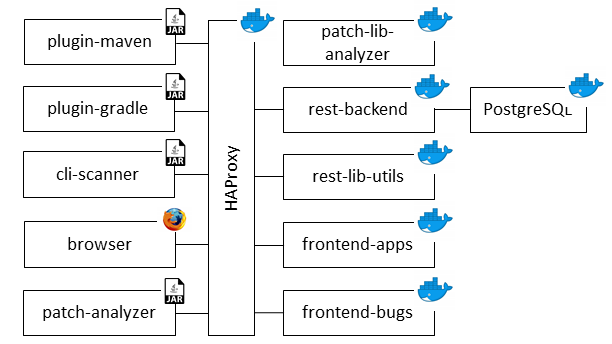
\includegraphics[width=\textwidth]{vulas_docker_architecture.png}
    \caption{vulas docker-compose architecture}
    \label{fig:vulas_docker}
\end{figure}

\begin{itemize}
\renewcommand\labelitemi{--}
    \item \textbf{frontend-apps}: \newline
    OpenUI5 front-end built for users to view different test results (\textbf{app} to generate a bill of material report, \textbf{a2c} to build call graphs, etc...). On this interface, users will be able to display all vulnerabilities discovered in their package, the dependencies affected as well as the reachable call graphs\autocite{Frontendapps}.

    \item \textbf{frontend-bugs}: \newline 
    OpenUI5 front-end for viewing results of scans (required when the AST method  previously described cannot yield a definitive result).
    
    \item \textbf{rest-backend} \newline 
    Springboot backend which interfaces with the vulnerability database and serves an API for all other services in the architecture.
    
    \item \textbf{rest-lib-utils} \newline
    Springboot backend which provides utilities for scanning such as pulling repositories from the respective source code repository and getting a list of dependencies from said archive.
    
    \item \textbf{patch-lib-analyzer}: \newline 
    Java application that establishes whether a library contains a construct modified to fix a vulnerability (aka changed-construct) in its vulnerable or fixed version. 
    
    \item \textbf{postgreSQL}: \newline Database storing information regarding CVEs, construct changes and application constructs.
    
    \item \textbf{HAProxy}: \newline High availability load balancing mainly used to serve the application. It is important to note that all communications between containers within the private Docker network and not through a domain name so this component is only mandatory if the application is to be exposed to the Internet.
\end{itemize}

\vspace{3mm}
A scan can be launched by either adding a plugin to the build process (either through the \textbf{plugin-maven} or \textbf{plugin-gradle}) or running a compile jar to scan a specific artifact (\textbf{cli-scanner}). In order to populate the database with known vulnerabilities, the \textbf{patch-analyzer} can load a series of CVEs crawled from the NVD database and finds the appropriate commit fix for each library. 

\newpage
\section{Orchestration in Kubernetes}

\hspace{5mm} Kubernetes, hereinafter referred to as k8s, is an open-source system for automating deployment, scaling and management of containerized applications. Due to it being a recent technology (released less than five years ago under the Apache License 2.0), this section attempts to summarize both its terminology and its overall orchestration mechanisms. For a more in depth understanding of its high level architecture, see Appendix (\ref{sec:high}). 

\subsection{Containers — A new era of deployment}

\hspace{5mm} The massive adoption of k8s marks the entry into a new era of deployment. Initially, deployments were applied directly onto physical servers. However, the \textbf{traditional deployment} era suffered from performance issues stemming from the inability to define resource boundaries between different applications. The introduction of \textbf{virtualization} tackles this issue by allowing multiple Virtual Machines (VM) to run on a single physical server. These VMs provide a level of security through isolation of scalable component as well as reduce the strain on hardware. Nonetheless, each VM is a full machine running its own operating system on top of the virtualized hardware. 

\vspace{2mm}
\begin{figure}[h]
    \centering
    \subfloat[traditional]{{\includegraphics[width=0.3\textwidth]{docker_deployment_trad.png} }}%
    \quad
    \subfloat[virtualized]{{\includegraphics[width=0.3\textwidth]{docker_deployment_vm.png} }}%
    \quad
    \subfloat[containerized]{{\includegraphics[width=0.3\textwidth]{docker_deployment_container.png} }}% 
    \caption{Evolution of deployments throughout the years}
    \label{fig:docker_evolution}
\end{figure}

\subsection{Docker Containers — Infrastructure base building block}

\hspace{5mm} At the forefront of this technology is Docker, a platform for developers and sysadmins to develop, deploy, and run applications with containers; a container being a standard unit of software that packages up code and all its dependencies so the application runs quickly and reliably from one computing environment to another.

\vspace{2mm} In order to instantiate a container, an executable package that includes everything needed for the application (runtime, libraries, code, configuration files) also known as an \textbf{image} is required. For example, a client can ask the docker daemon to pull an Ubuntu image from a registry (public or private) which can then be instantiated as containers in the host machine. Nowadays, the docker daemon is broken up into three main components:

\begin{itemize}
    \item \textbf{runC} is the lowest level runtime component used to interact with the OCI (Open Container Initiative) interface. This module interacts directly with the kernel in order to create namespaces, cgroups, capabilities, and filesystem access controls. In practice, a container is an environment running in an isolated set of kernel namespaces (see Appendix (\ref{appendix:libcontainer})) .
    \item These container lifecycles are then managed by the \textbf{containerd} daemon which also takes care of setting up the networking and image transfer.   
    \item Finally, the \textbf{Docker engine} only provides high level CLI for users and downloading images from docker registries. 
\end{itemize}

\begin{figure}[h]
    \centering
    \includesvg[width=0.8\textwidth]{docker_oci.svg}
    \caption{Docker low level architecture}
    \label{fig:docker_depth}
\end{figure}


\subsection{Kubernetes Objects — Base k8s abstractions}

\hspace{5mm} Kubernetes objects are abstractions that represent the state of the system. These persistent entities describe what containerized applications are running, the resources allocated and available as well as their behaviors (restart policies, fault-tolerance). Unlike normal infrastructure declaration, these objects portray the desired state of the cluster which k8s will try to satisfy. This “record of intent” is declared in a declarative fashion in \textbf{yaml} and interpreted by \textbf{kubectl}, k8s's default CLI (An example of a simple nginx declaration can be found in Appendix (\ref{sec:declaration})).


\subsubsection{Pods — Base execution unit}

\hspace{5mm} A Pod is k8s's basic execution unit, a process running on the Cluster similar to a container in a monolithic deployment. Unlike its counterpart, a Pod declares an unit of deployment and thus can be used in two ways:
\begin{itemize}
    \item \textbf{Single container} pods which encapsulate the container serving as an adapter for k8s to better manage said container (with resources needs, volumeMounts etc...)
    \item \textbf{Composite container} pods which wraps multiple containers that are tightly coupled and need access to a shared resource. This approach although less common in practice allows for the implementation of design patterns which help solve and reuse common problems with distributed architectures.
\end{itemize}

One of the most important concept related to pods is that they follow an \textbf{ephemeral lifecycle}, they are not meant to survive if a failure of any kind were to occur (scheduling failure, node failure, lack of resource, etc...) and do not self heal in order to reach the desired state. Therefore, Pods are rarely individually created but provisioned by high level abstractions called \textbf{Controller}. A pod's lifecycle can be summarized as follows:

\begin{figure}[h]
    \centering
    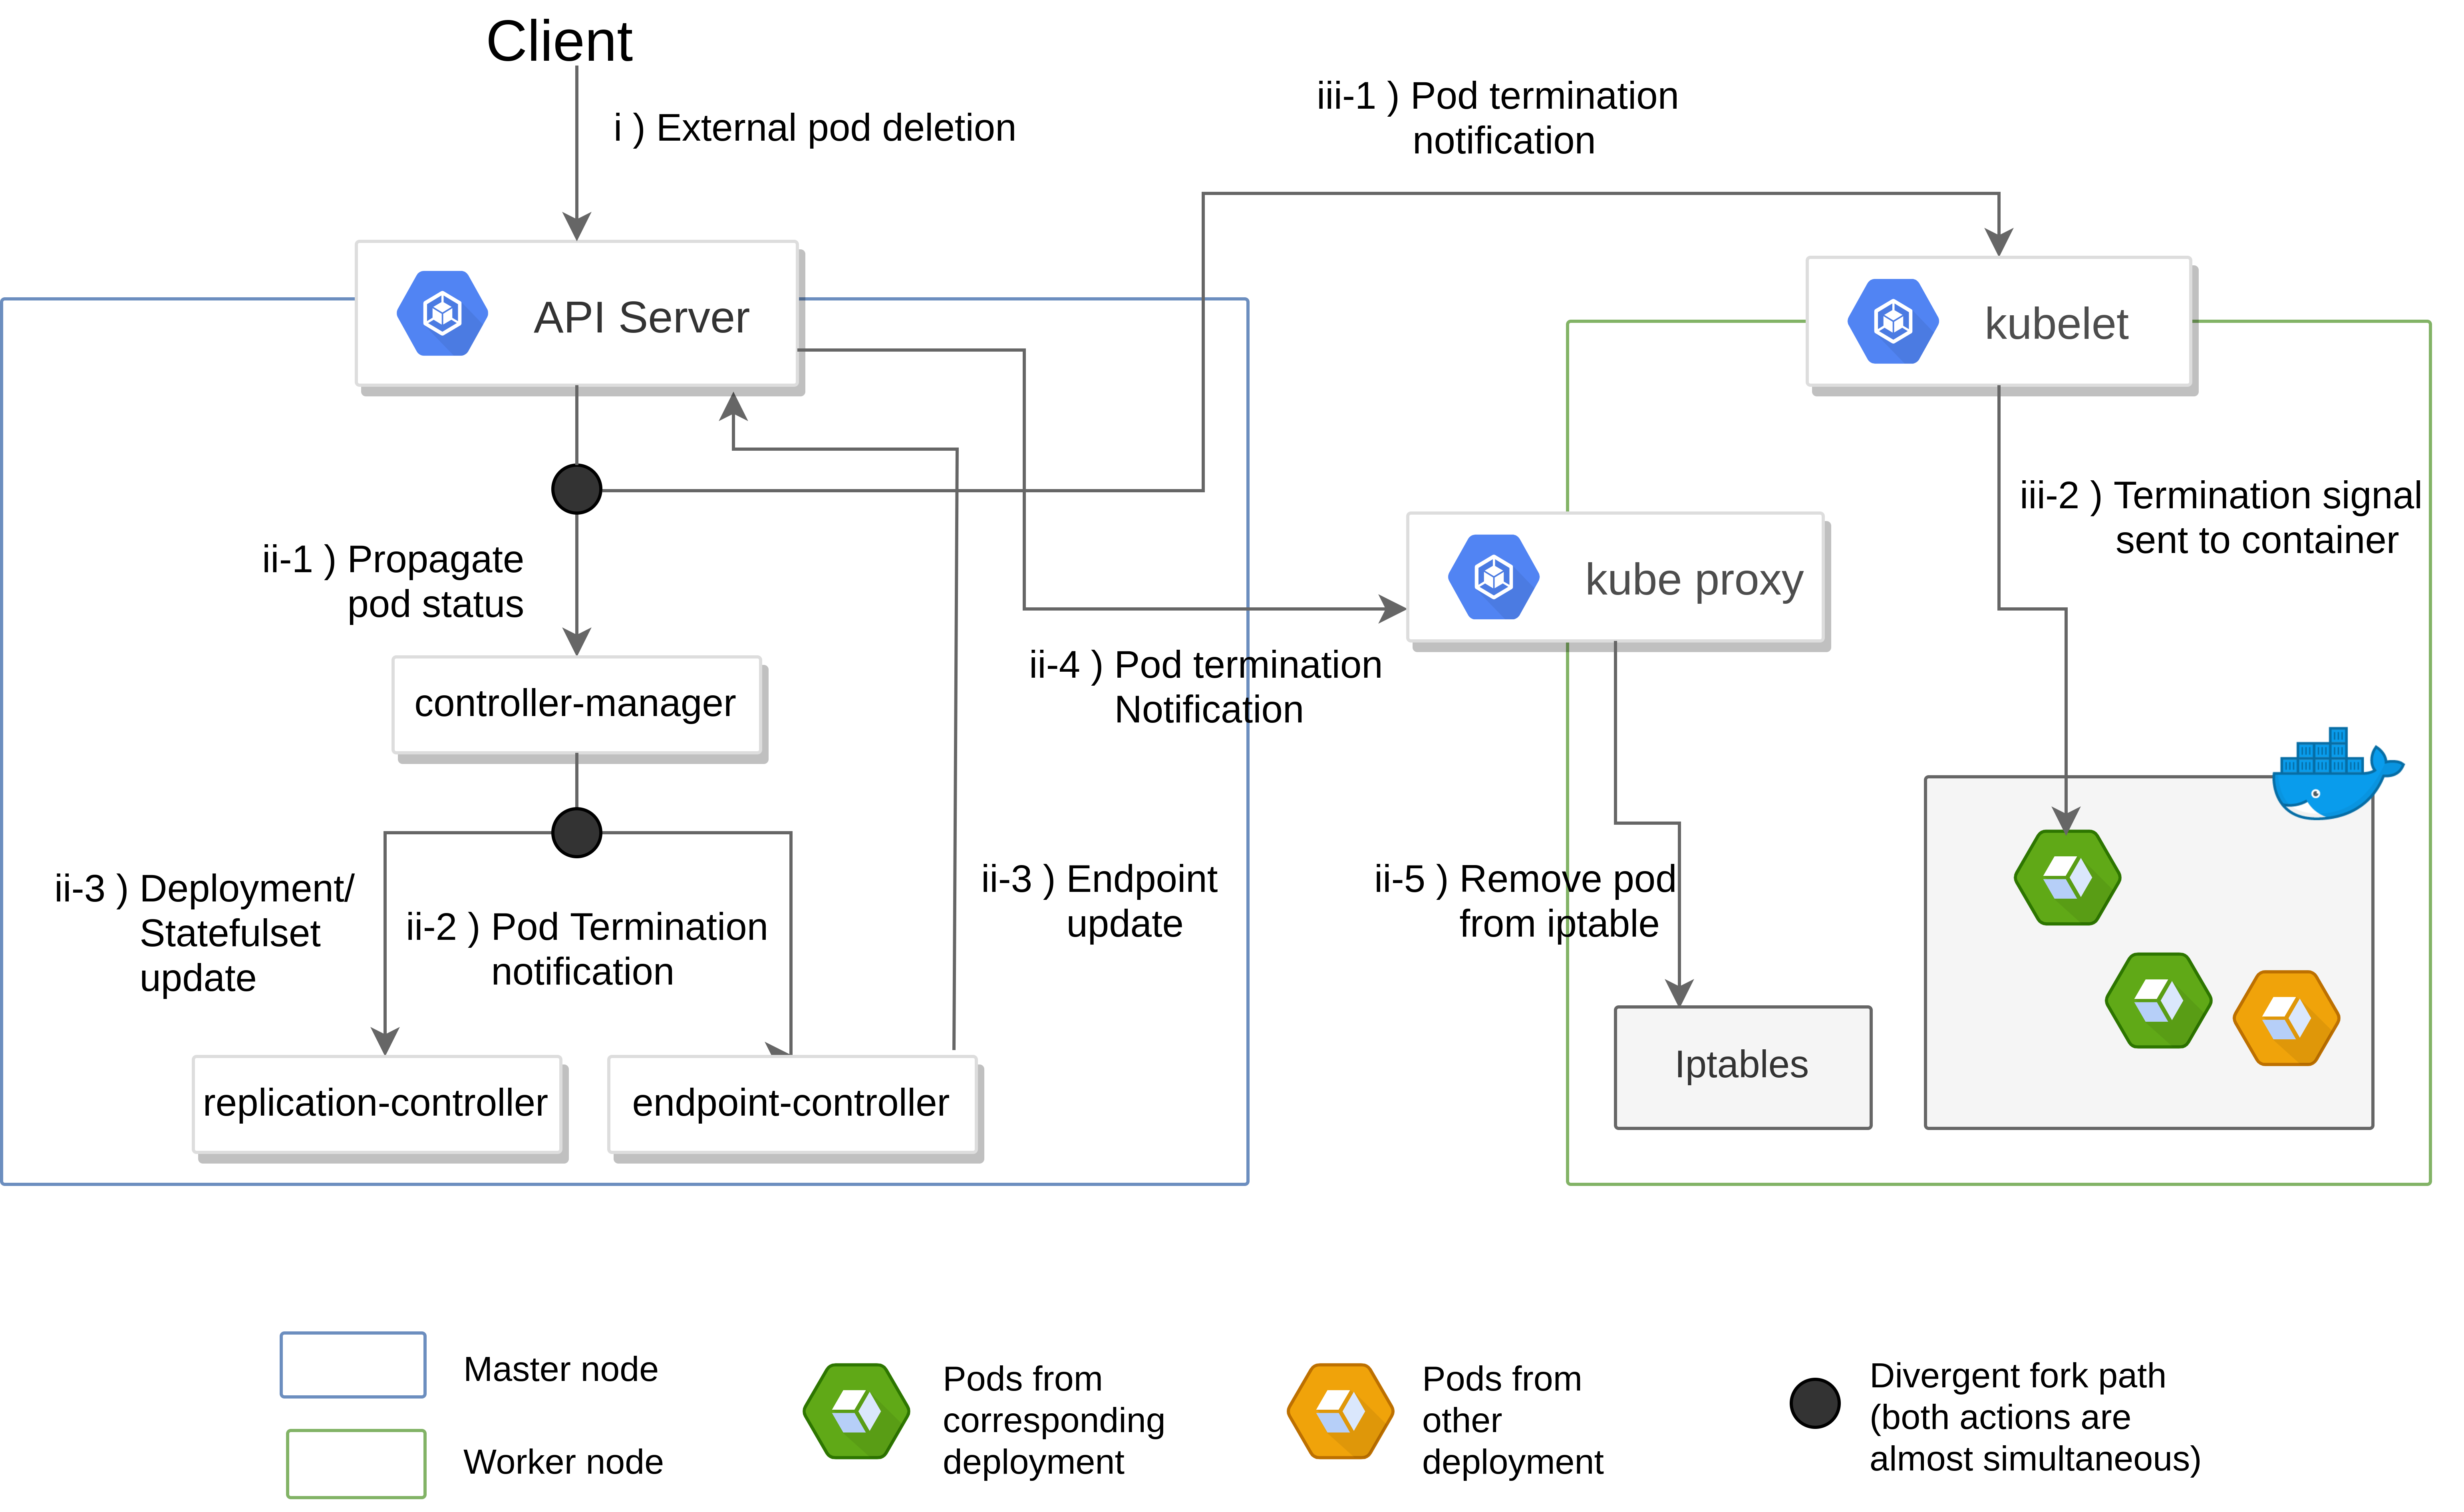
\includegraphics[width=\textwidth]{k8s_lifecycle.png}
    \caption{Simplified diagram for termination of a pod}
    \label{fig:pod_end}
\end{figure}

\begin{enumerate}[i)]
    \item \textbf{Scheduling}: \\[0.1cm] A controller requires the creation of a pod to satisfy its desired state and communicates it to the k8s API. A pod with the corresponding specs is then scheduled for creation.
    
    \vspace{1mm}
    \item \textbf{Lifespan}: \\[0.1cm] If the resources demanded can be satisfied in a node, it is assigned an unique ID (UID) and will remain bound to that node until termination or deletion. 
    
    \vspace{1mm}
    \item \textbf{Termination}: \\[0.1cm]  If the restart policy is set to "Always", the pod would be restarted (maintaining the same UID) no matter the exit code of the encapsulated containers. A restart policy set at "OnFailure" would do the same thing but only with non error exit codes. Finally, a "Never" restart would lead to the termination of the pod. Non persistent associated volumes would then be unmounted, allocated resources freed, kube-proxy iptables update and bound endpoints removed.
\end{enumerate}

\subsubsection{Services — Base networking unit}

\hspace{5mm} As most components in k8s are not durable, keeping track of which IP to connect to in order to link up components over the network is impossible, thus making an abstraction like Services mandatory. Services in k8s define a logical set of Pods determined by a selector to connect to rather than a fixed set of IPs which allow for dynamic internal routing for deployments that do not care which instance handles the routed request. In practice, service selectors are used to match with labels meaning that only objects having said labels can communicate using the aforementioned service. Services can then be put into three main categories (see Figure (\ref{fig:k8s_service_type})).
    
    \begin{figure}[h]
        \centering
        \subfloat[ClusterIP]{\includegraphics[width=0.3\textwidth]{k8s_service_cluster_ip.png}}
        \hspace{2mm}
        \subfloat[NodePort]{\includegraphics[width=0.3\textwidth]{k8s_service_node_port.png}}        
        \hspace{2mm}
        \subfloat[LoadBalancer]{\includegraphics[width=0.3\textwidth]{k8s_service_load_balancer.png}}       

        \caption{Kubernetes service types}
        \label{fig:k8s_service_type}
    \end{figure}
    
    \vspace{3mm}
    \begin{enumerate}
        \item \textbf{ClusterIP} : the default service type in k8s ensuring that a given set of destination ports on a set of machines that match the selector are reachable only from within the cluster. For example, if a ClusterIP service with the name \textit{nginx-service} in the \textit{default} namespace is defined and targeting an nginx deployment, all pods within that namespace can communicate with the nginx pods through the domain name \textit{nginx-service.default.svc.cluster.local} at the ports declared. 
        
        \item \textbf{NodePort} : exposes the service to external traffic by opening specific ports on all nodes. Requesting \textit{NodeIP:NodePort} would be permitted from outside the cluster, introducing a major security concern.
        
        \item \textbf{LoadBalancer} : exposes a service to the Internet assigned to a fixed external IP to the Service (the creation of the external IP often being relegated to the cloud provider). 
        
        \item \textbf{ExternalName} : maps a service to a CNAME record (e.g. foo.bar.com). Extremely useful for mapping external services such as a database with a floating IP outside of the cluster. 
    \end{enumerate}

\subsubsection{Ingresses — External access API} \label{sec:ingress}

\hspace{5mm} Ingresses provide a mean for services in a cluster to be accessible from the exterior either through HTTP or HTTPS. It can be configured to give Services externally-reachable URLs, load balance traffic, terminate SSL / TLS, and offer name based virtual hosting but requires an Ingress Controller to fulfill its task.

In usual deployment scenarios, a LoadBalancer is used to expose the Ingress Controller deployment which then manages and routes requests according to the ingresses defined.  

\subsubsection{Volumes — Base storage unit} \label{sec:k8s_volumes}
\hspace{5mm} The ephemeral nature of containers also has its impact on storage. A k8s volume's lifecycle strictly follows that of the Pod that encloses it. Therefore, a volume bound to a pod outlives any containers allowing for data to be preserved across container restarts. 

In order to avoid confusion going onwards, the following terms will be used:
\begin{enumerate}
    \item A volume is \textbf{bound} to a pod once its declared in the \textit{.spec.volumes} field
    \item That volume could then be \textbf{mounted} to any numbers of containers within that pod simultaneously once its declared in the \textit{.spec.containers.volumeMounts}
\end{enumerate}

\vspace{2mm} Kubernetes supports a myriad of volume types that differ in their storage implementation and their initial contents.

\subsubsubsection{Persistent Volume Claim}

\vspace{-5mm} Persistent Volume Claims (PVC) is the most common volume type, providing an abstraction as to how storage is provisioned and consumed independently of the cloud environment. 

In order to provision a PVC, an actor states a claim to durable storage backed by a Persistent Volume (PV). Note that, a PV's lifecycle is managed by k8s independently of any object that mounts it, thus, making it non ephemeral. Furthermore, a storage class can be defined to enrich the volume's feature such as volume expansion and reclaim policies. Therefore, an object can consume storage resources in an agnostic manner, having no prior knowledge of the storage class nor the private volume satisfying the claim (Figure (\ref{fig:k8s_pv}) goes into detail how Openstack provisions PVs).

\begin{figure}[h]
    \centering
    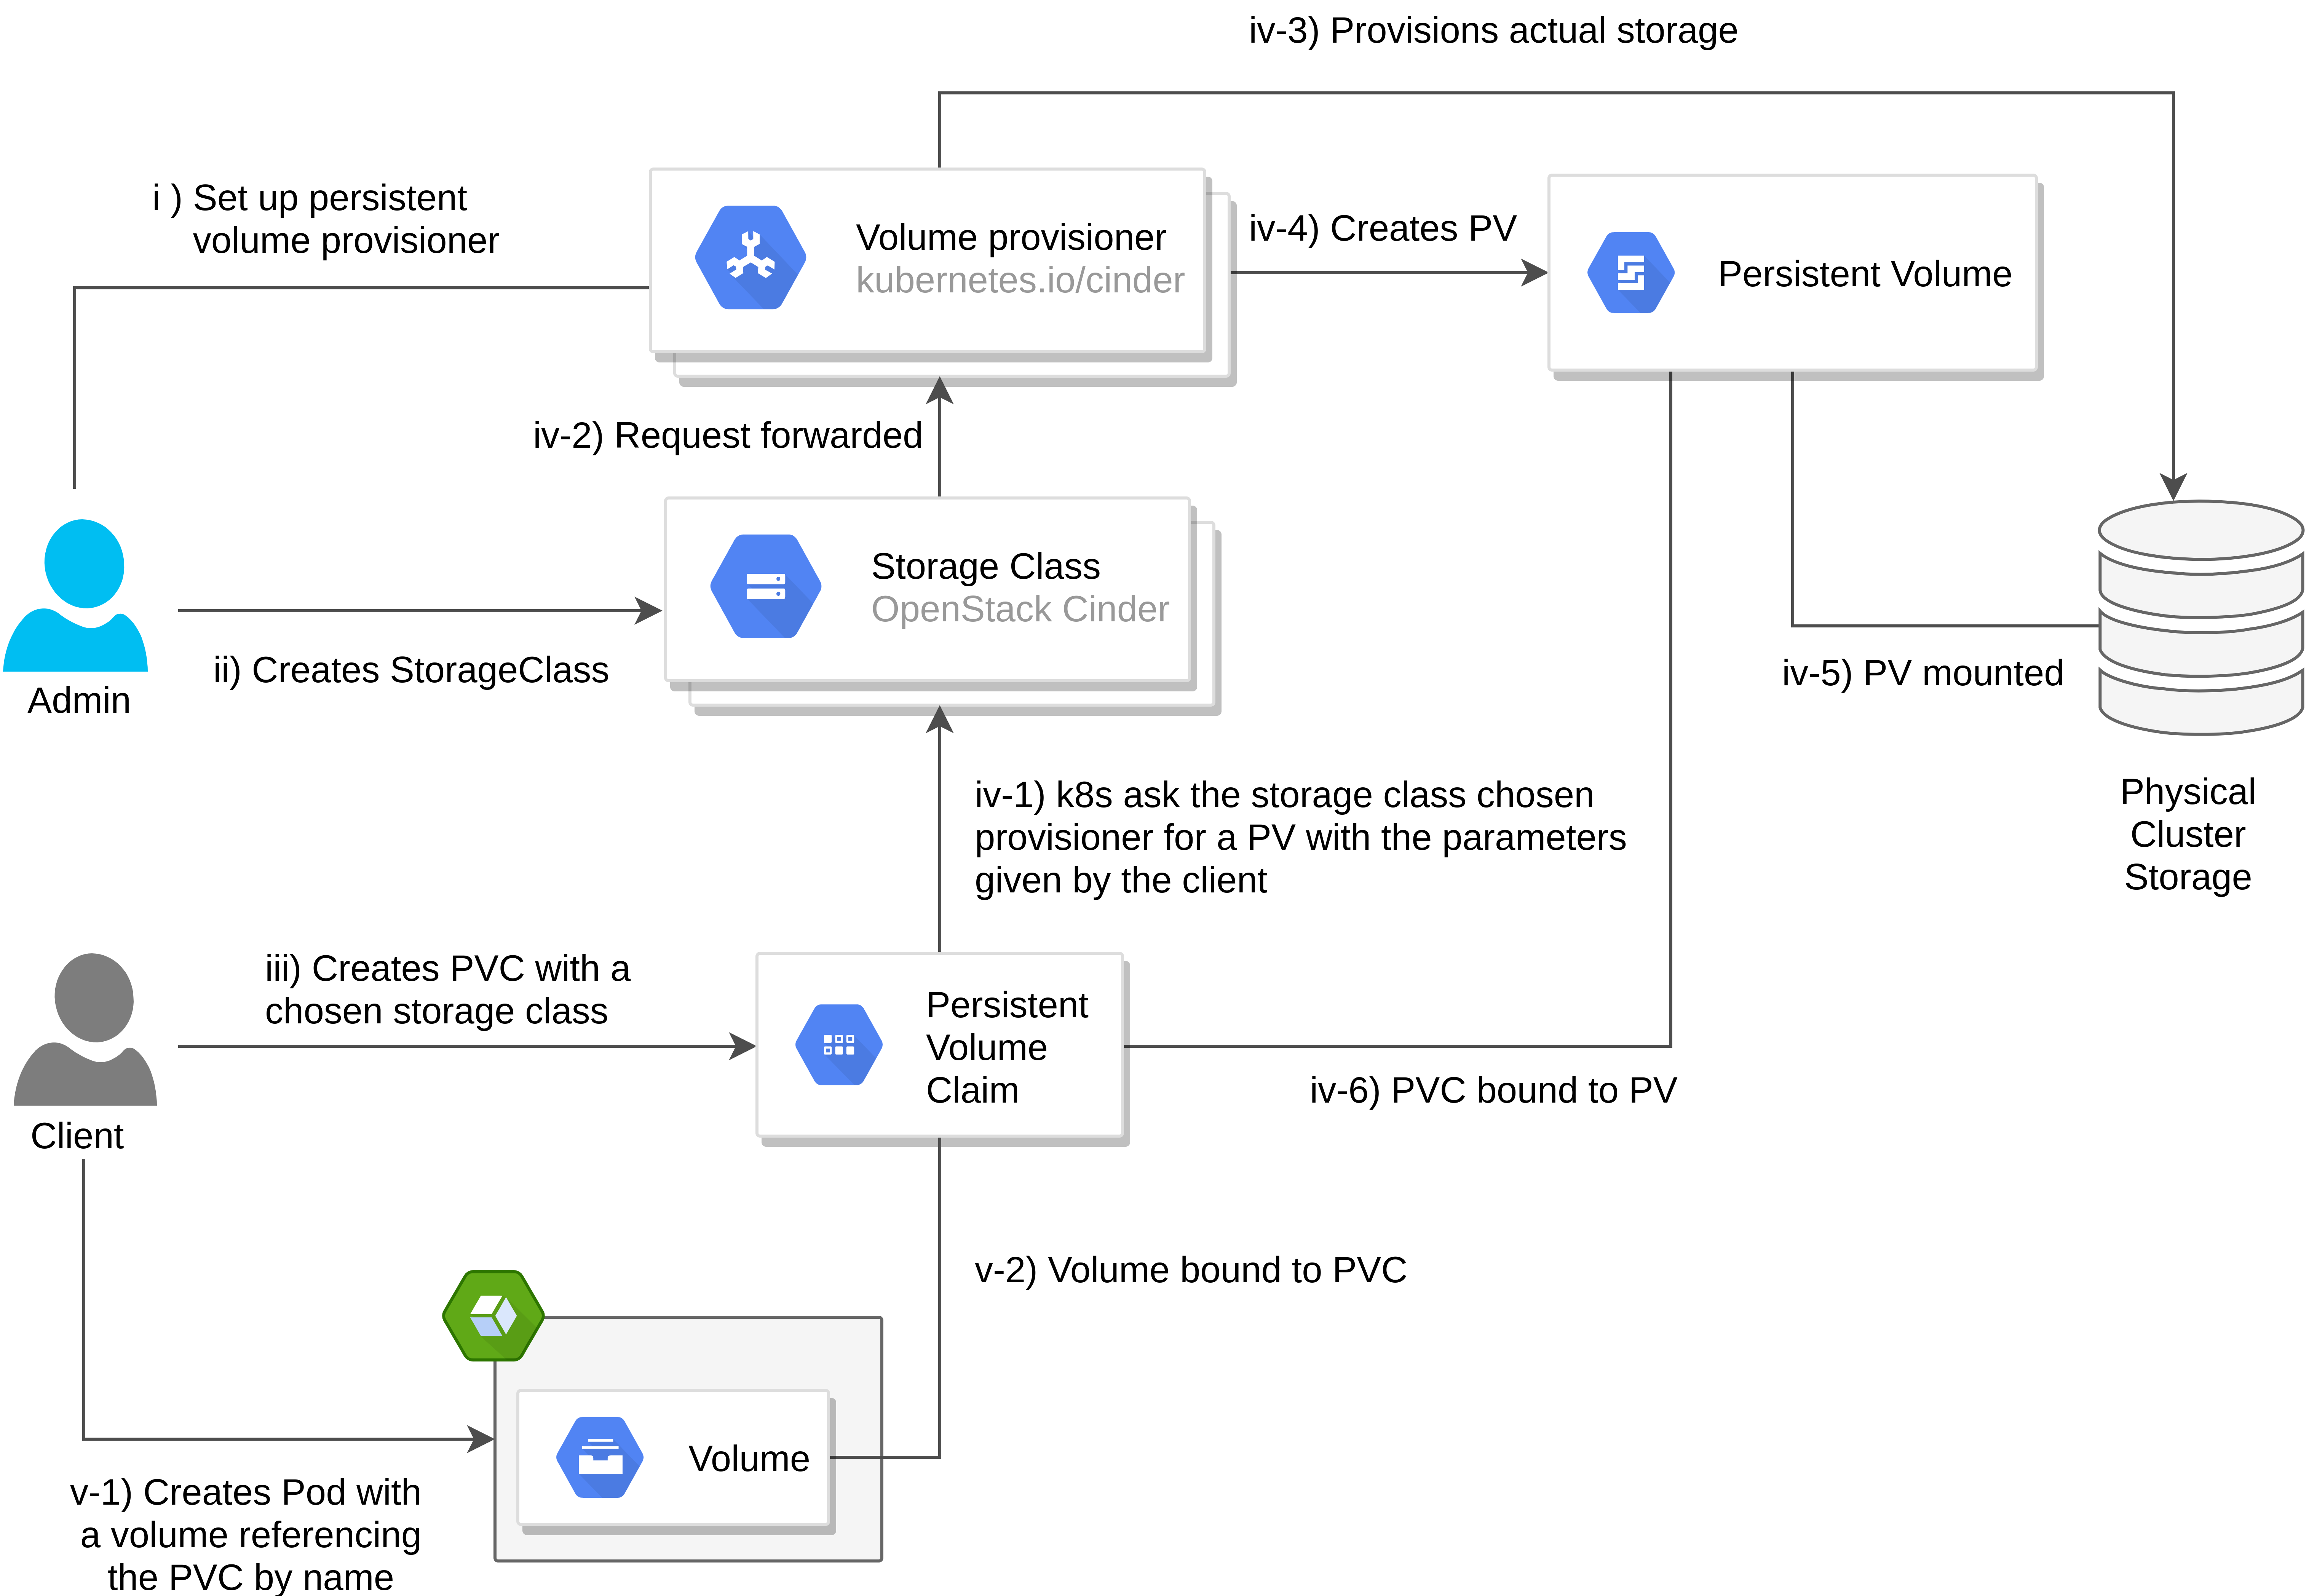
\includegraphics[width=0.95\textwidth]{k8s_pv.png}
    \caption{Openstack Cinder PV provisioning mechanism}
    \label{fig:k8s_pv}
\end{figure}

\subsubsubsection{HostPath}

\vspace{-5mm} A HostPath volume mounts a file or directory from the host node’s filesystem into the given pod. This volume type permits applications to access to Docker internals through /var/lib/docker or to interface with the kernel through /sys and thus, mandatory for native k8s monitoring. 

\subsubsection{Controllers}

\hspace{5mm} As previously stated, Pods were not designed to be created individually but by \textbf{controllers}; high level abstractions that ensure the desired state of the cluster matches the observed state. 

\subsubsubsection{Deployments}

\vspace{-5mm} Arguably the most commonly used controller, the Deployment controller encapsulates Replicasets and Pods in the k8s's resource hierarchy. The \textbf{Replicaset} object being k8s's main mechanism to managing scaling of pods (ReplicationController being deprecated) which is used to maintain a stable set of replica Pods adhering to a given Pod template manifest, running at any given time. 

Since this API object is meant to be a low level object, \textbf{Deployments} are built upon ReplicaSets to offer a wider range of usages. One of those usage being \textbf{rollout} and \textbf{rollbacks} which help solve problems with updating and reverting Pod templates whilst maintaining all the service provided by the cluster. A Rolling Update, the default update strategy for k8s deployments represent in practice a blue-green deployment technique (see Figure (\ref{fig:k8s_rollout})).

\vspace{5mm}
\begin{figure}[h]
    \centering
    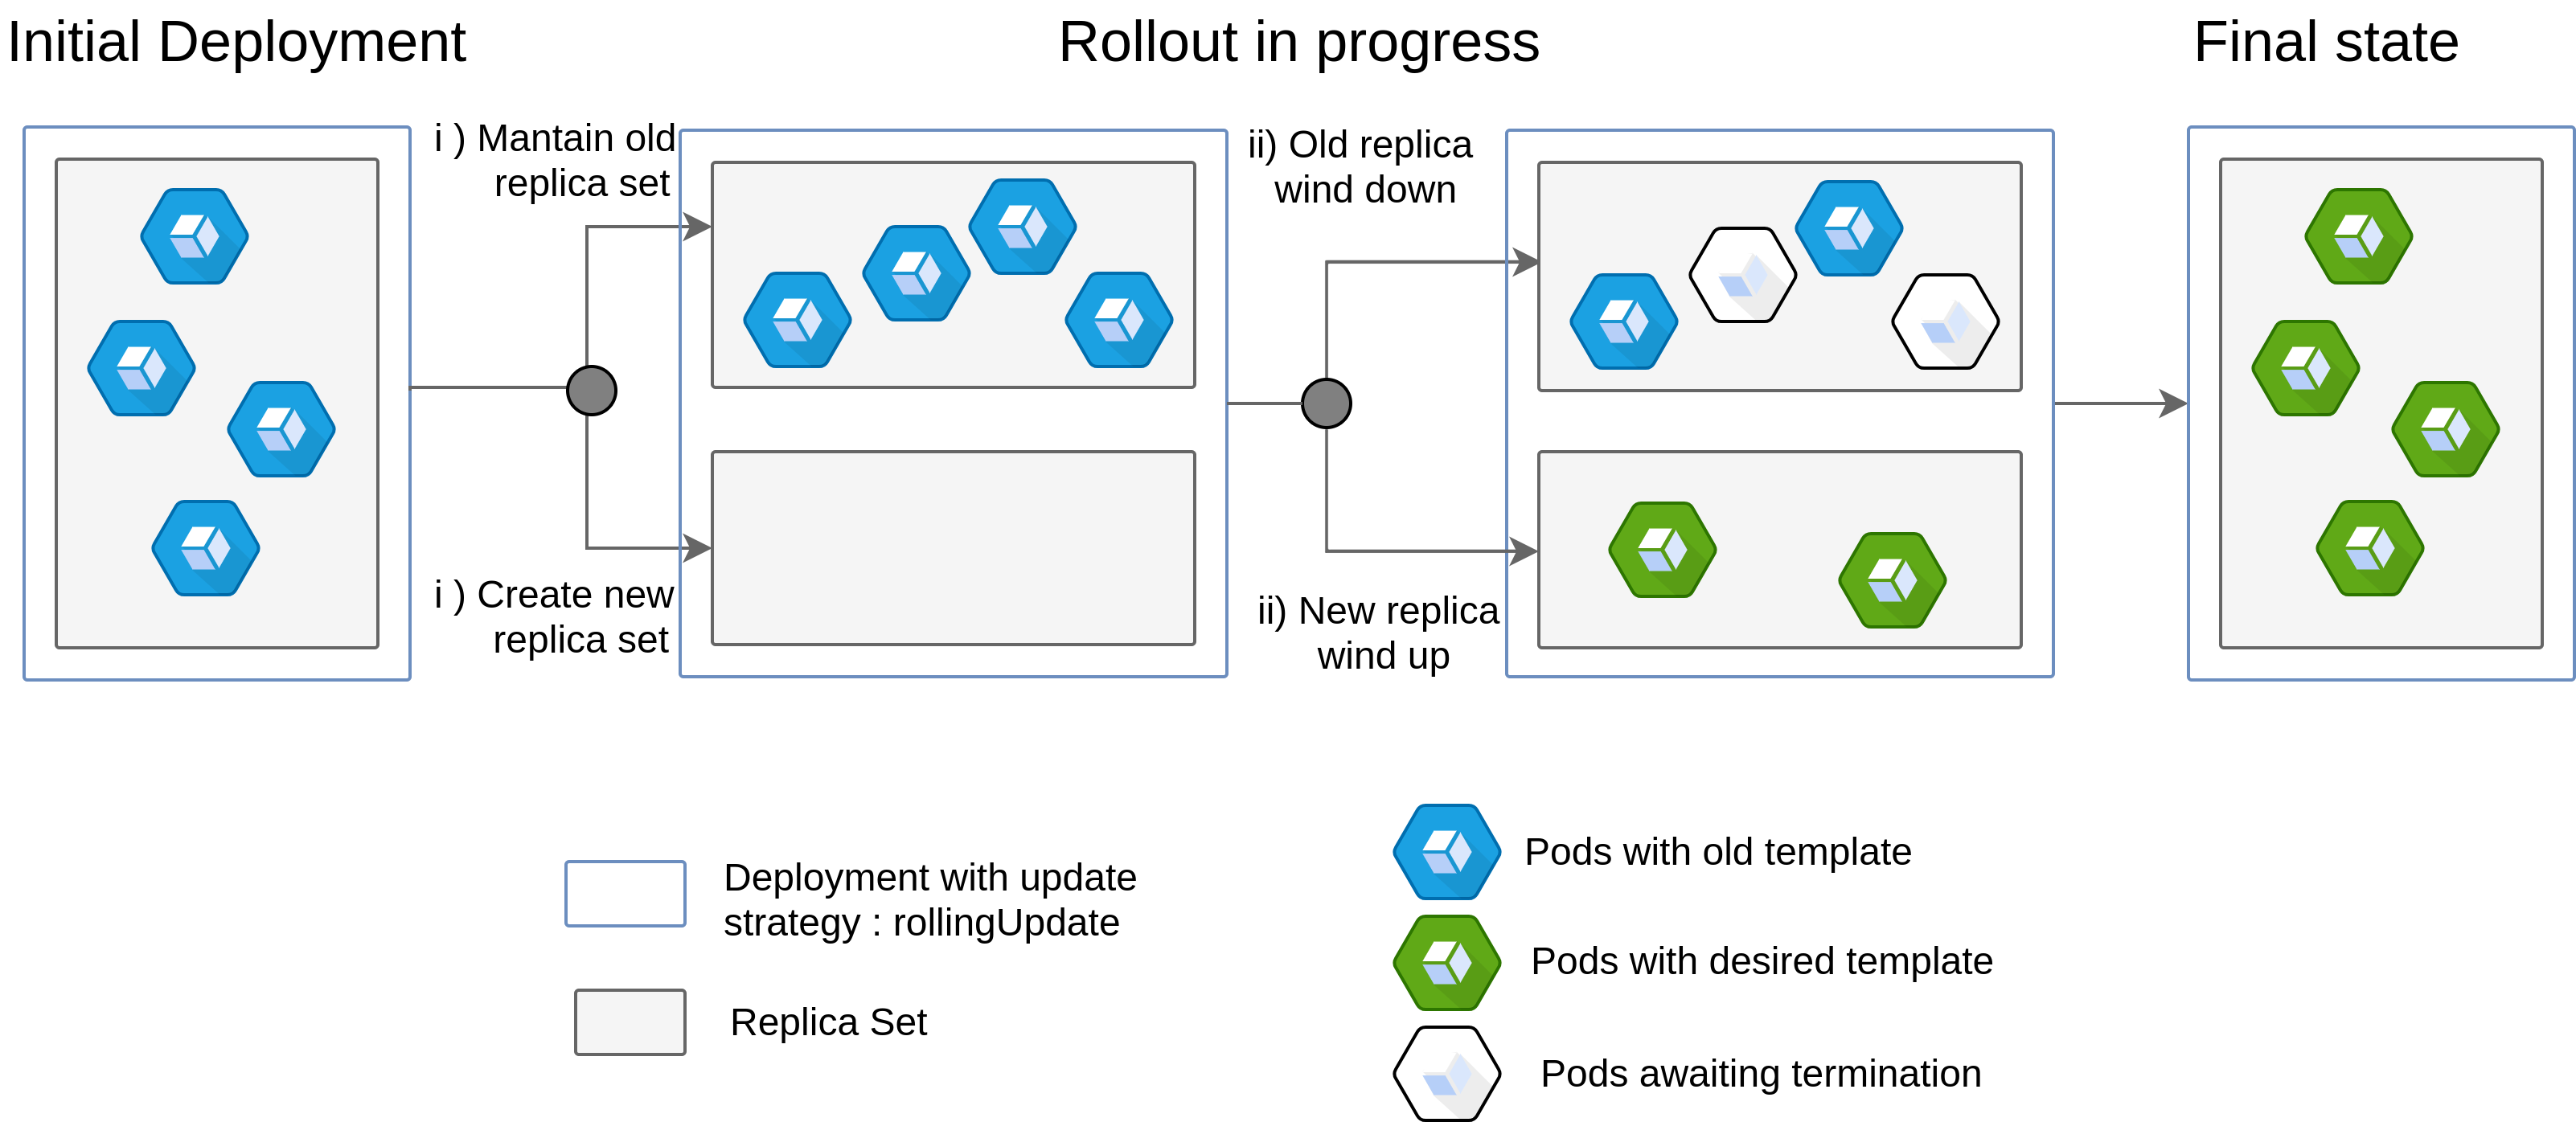
\includegraphics[width=\textwidth]{k8s_rollout.png}
    \caption{k8s blue green deployment rollout}
    \label{fig:k8s_rollout}
\end{figure}

\subsubsubsection{Statefulsets}

\vspace{-5mm} A Statefulset is quite close to a Deployment but adds a sticky identity for each of their Pods. This persistent identity allow for stable (persistent across pod scheduling) and ordered deployment and scaling. 

For instance, in a statefulset comprising of N replicas, each pod will be created sequentially in order from \{0..N-1\} and assigned an unique ID in that same range. As the goal of statefulset is overall order, termination of a Pod is only available once all its successors are terminated and scaling up require that all predecessors are Running and Ready. However since it does not create ReplicaSets, rolling back a Statefulset to a previous version is impossible.

\subsubsubsection{Daemonsets}

\vspace{-5mm} The least commonly used controller are Daemonsets which ensure that a copy of a Pod is run on a certain set of nodes. Its main usage case are node monitoring daemons (Prometheus for instance), logs collection daemons or cluster distributed storage daemon such as ceph.

\subsection{Helm — Configuration management for k8s}

\hspace{5mm} Managing k8s's complex environment and deployment can be done either through Helm, Kustomize or natively and therefore a technical choice has to be made for the vulnerability-assessment-tool's case. 

\textbf{Kustomize}

Kustomize is a k8s native configuration management not based on templating but rather on raw, hard-coded, static YAML declarations. These declarations when added together in a $kustomization.yaml$ (see Figure (\ref{fig:kustomization})) allow for development, staging and production environments to coexist. With features such as \textit{secret generator} and \textit{config generator}, this tool can update secrets and configmap and keep them separate from the static object statements. 

If the k8s deployment were to be changed and published to the public repository, an user would have to: git pull from the latest branch, resolve conflicts if they made any changes to the files, apply the kustomize CLI to apply the changes.

\textbf{Helm}

Helm is a package manager for k8s which helps define, install, and upgrade even the most complex k8s application. Unlike Kustomize, Helm uses the concept of Charts, a set of templated yaml declarations with a "variable" file named $values.yaml$ to provide repeatable update and rollbacks through each new release of the latter (see Figure (\ref{fig:helm})). 

Although developing a chart is quite complex (due to the complexity of the Golang templating engine used), if published, it can facilitate k8s deployment for users of the open-sourced tool. On the consummer's side, fetching an update to the Chart from version $a$ to version $b$ translates to running a single command: \shellcmd{helm upgrade CHART\_NAME}

\vspace{3mm}
\textbf{Conclusion}

Taking the potential consumer's of the vulnerability-assessment-tool into consideration, it was concluded that a helm chart would be developed and open sourced. The idea behind this was to allow multiple organizations and individuals to have their own instances of the tool and share their assessment regarding certain CVEs in a collaborative document store (described further in Section \ref{sec:vulnkb}). In the future, the chart would be submitted to the official chart registry \footnote{source: https://github.com/helm/charts} as an incubator project then progressively matured into a stable one.

\newpage
\section{Migrating Vulas to the Cloud}

\subsection{Current setup and reasons for the migration} \label{sec:reason}

\hspace{5mm} The current production deployment of the vulnerability-assessment-tool is based upon docker-compose (see Figure (\ref{fig:vulas_core01})) and centers around 5 machines hosted by Converged Cloud (SAP's private cloud provider):

\begin{itemize}
    \item \textbf{core-01}: hosts all the containers, volumes that are prevalent to production (every component listed in Section (\ref{implementation}) along with a proxy for exposing the service (in our case an HAProxy container) as well as some cron-jobs designed to initiate database backup and stats collection.
    \item \textbf{test-01}: carbon copy of the previous machine but destined to be the staging area (thus, subject to extensive testing and monitoring) before deploying to production.
    \item \textbf{dev-01}: carbon copy of the core machine used for pushing releases with potentially unsafe changes (both code wise and infrastructure wise). 
    \item \textbf{monitoring-logging-01}: passive centralized monitoring (prometheus, grafana) and logging (kibana, elasticsearch) receiving logs (from the rsyslog daemon running in each machine) and metrics (node metrics from cadvisor and database metrics from the postgres exporter) from each machines (see Figure ).
    \item \textbf{patch-01}: machine only dedicated to periodically run the patch-lib-analyzer job to assess vulnerabilities from scanned libraries.
\end{itemize}

\vspace{2mm}
As Converged Cloud is based on Openstack (which allows for controlling large pools of compute, storage, and networking resources throughout a datacenter), the machines were created using the UI and provisioned using \textbf{Ansible playbooks} specific to each usage. Shell scripts calling docker-compose were then created for every specific situation (backing up the database, resetting the proxy configuration, publishing a new release, etc...).

The migration to the cloud intends to address the following concerns with the current stack: \label{sec:obj}
\begin{enumerate}
    \item \textbf{Not highly available}: \label{obj:dep_ha} although the containers are redundant within each node, the deployment itself is not resilient to outage occurring on a specific node.
    \item \textbf{Spin up duration}: \label{obj:dep_spin} due to its reliance on automating system requirements provisioning through Ansible, if a node were to go down, the time required to spin up a new functional instance would entail high downtime.
    \item \textbf{Overhead cost}: \label{obj:dep_overhead} each maintenance operation (database backup, smoke test) requires a specific Ansible playbook that has to be maintained and updated. At the same time, publishing new releases of the software solely relies on docker-compose and thus, is quite complicated.
    \item \textbf{Non reproducible heterogeneous infrastructure} \label{obj:dep_reprod} due to an UI based infrastructure creation, and each machine serving different purposes.
\end{enumerate}

\subsection{Overview of choices and challenges}

\hspace{5mm} Since the application was not developed with the intention of being used in the k8s/cloud native environment, the migration to the cloud requires a lot of technical choices and challenges that will detailed in the following sections:
\begin{itemize}
    \item \textbf{Database management}: migrating the vulnerability-assessment-tool to k8s
    \item \textbf{Core components}: transitioning all the components vital to having a functional deployment of the vulnerability-assessment-tool (see Section (\ref{implementation}))
    \item \textbf{Support stack}: adapting components destined to serve the tool over the Internet
    \item \textbf{Monitoring stack}: translating the monitoring and logging functionality stack to a more cloud native version. 
    \item \textbf{Infrastructure provisioning}: creating the underlying machines and networking components required for running k8s.
\end{itemize}

\subsection{Database management}

\hspace{5mm} The vulnerability database is at the heart of the tool, storing construct changes, CVE information, vulnerable constructs discovered in scanned applications, etc... This database requires that a couple properties be respected:

\begin{itemize}
    \item \textbf{Persistence}: data stored in the database should not be deleted by external processes or objects until the user deletes it. It should withstand outages (maintenance operation, schema change, node failure, disk failure, etc...).
    \item \textbf{Coherence}: any given database transaction must change affected data only in permitted ways and any transaction started in the future necessarily sees² the effects of other transactions committed in the past. 
    
    \item \textbf{Performance}: queries should be resolved at the lowest latency possible for the lowest amount of resources allocated possible. This dual optimization will require an in-depth study of a sample of commonly used queries.
    
    \item \textbf{Schema change} and \textbf{Rollback}: the schema of the database is prone to change over different releases. This change is propagated to the database through the rest-backend thanks to the Flyway framework attached to the rest-backend component. The selected management method should allow for rollbacks if this migration were to fail and revert from the corrupted data set to a functional state whilst minimizing downtime.
    
    \item \textbf{Backup} and \textbf{Recovery}: production critical data should be periodically backed-up so that any disk outage should be recoverable.
\end{itemize}  

\newpage
In order to fully benefit from a cloud based deployment, it should also satisfy \textbf{High Availability} (maximize resilience against node failure achievable through data partitioning). However, as per the CAP theorem (see Figure \ref{fig:vulas_cap}), these goals cannot be reached as a database cannot simultaneously be \textbf{Consistent}, \textbf{Available} and \textbf{Partitioned}.

\begin{figure}[h]
    \centering
    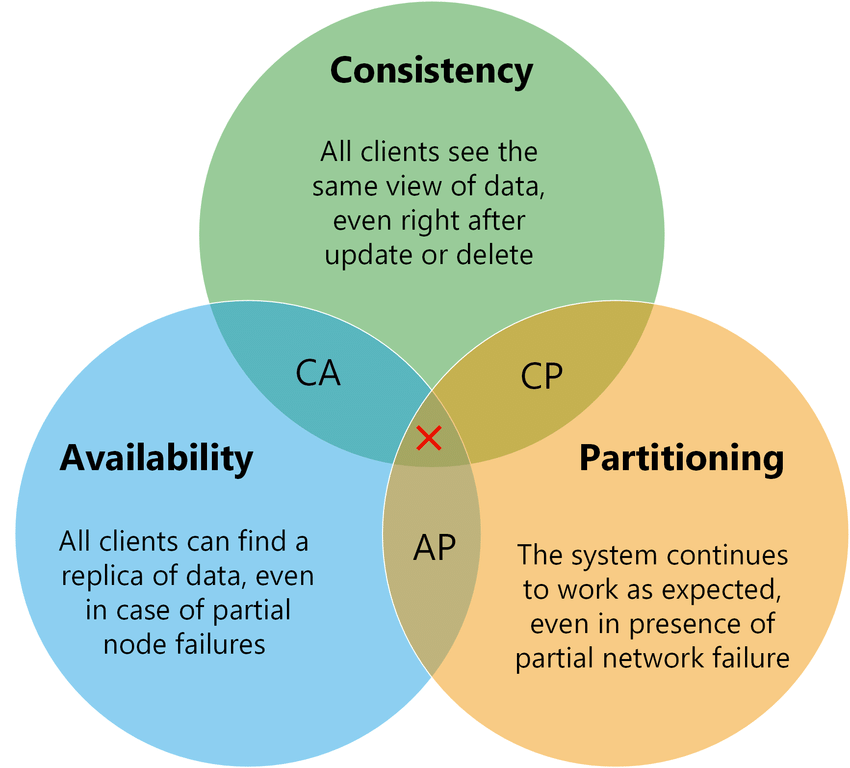
\includegraphics[width=0.65\textwidth]{vulas_CAP.png}
    \caption{CAP Theorem \cite{CAP}}
    \label{fig:vulas_cap}
\end{figure}

Therefore, some trade-offs are to be expected in the final product and one can only maximize two of the previously mentioned attributes at the expense of the third. The CAP theorem is however a point of contention because distributed systems more often than not attempt to maximize each property whilst not fully satisfying any. 

\vspace{5mm}
\subsubsection{Reaching High Availability}

\subsubsubsection{Availability and Partitioning through NoSQL: }

\vspace{-5mm}\hspace{5mm} Achieving these properties can be done through a migration to a NoSQL database. Column oriented database such as Scylla/Cassandra can be an appropriate candidate given a replication factor of 2 or higher. This will require a remodelling of the database scheme by defining the most appropriate partition and sort keys. Some refactoring of the internal application logic is also required to implement data ingestion. 

This option would lower the operational cost of managing the database, with the clustering and availability delegated to the DBMS. However, the lack of consistency is not appropriate for the application at hand, as all clients should have the same view of the critical data of a given scan. After considering the available development resources, the refactoring task has also been deemed improbable in the near future. The cost of migration and these problems make a shift to NoSQL infeasible.

\vspace{3mm}
\subsubsubsection{Eventual consistency with SQL to reach HA}

\vspace{-5mm} An SQL database can be clustered in order to reach High Availability in exchange for some loss in strong consistency. A couple of solutions are to be considered:

\begin{enumerate}
    \item \textbf{MySQL managed clustering}: MySQL offers in-built functionalities for creating a master-slave cluster. Since the current database is already SQL and abstracted through Hibernate, a migration to this model would entail no development cost. 
    
    However, MySQL is distributed under a convoluted GPL license which stipulates that a closed-source redistribution of MySQL must enter into a commercial license agreement with Sun (the owners of the intellectual property). Since the vulnerability-assessment-tool has two "versions" (an open source one which obfuscates some of the internal one's source code), this decision would require purchasing a license.

    \item \textbf{Database sharding}: Hash based or manual sharding can be implemented software side in order to split the data load into multiple consistent SQL instances. As the development cost of such a model would be exorbitant, this solution is not to be considered despite its benefits to both scalability and performance.
    
    \item \textbf{PostgreSQL self-managed "clustering"}: this uses the master slave replication feature offered in order to create multiple eventually consistent read replicas. This option entail the highest operational cost (for managing the database, backups, etc...) in pursuance of the lowest development cost as well as the most flexibility.
\end{enumerate}

\label{sec:vulas_db_replication}
Due to the advantages described above, the k8s deployment will implement a postgres cluster with master slave replication. This method, called \textbf{Streaming Replication}, ensures that a standby server to stay more up-to-date than is possible with file-based log shipping. It streams WAL (Write Ahead Logs, transaction logs that are written to stable storage) records to the standby as they're generated, without waiting for the WAL file to be filled. Streaming replication being asynchronous by default (there is a small delay between committing a transaction in the primary and the changes becoming visible in the standby), strong consistency is not achieved. However since the delay is negligible, the data is eventually consistent all throughout the cluster.
 
In order to persist volumes on the same node and preserve a meaningful cache, database pods should, once created, stay on the same nodes. A stateful set is therefore the most appropriate controller for this case. As this is a master-slave architecture, the master pods and slave pods are heterogeneous and should therefore be declared in two different stateful sets. In order to set up replication between the master and slaves, the following steps are performed (see Figure (\ref{fig:vulas_master_slave})):

\begin{enumerate}
    \item The init container in the postgres replica pod uses \textbf{pg\_basebackup} pointed to the postgres master container. This command copies the data from the master node to make sure that the replica is up to date, then generates the replica.conf file which tells the replica node that it is the master's standby.  
    \item Once the base backup succeeds, the postgres replica container can spin up whilst mounting the same PVC as the init container (thus sharing the data stored in /var/lib/pgdata/data as well as the config files)
\end{enumerate}

\begin{figure}[h]
    \centering
    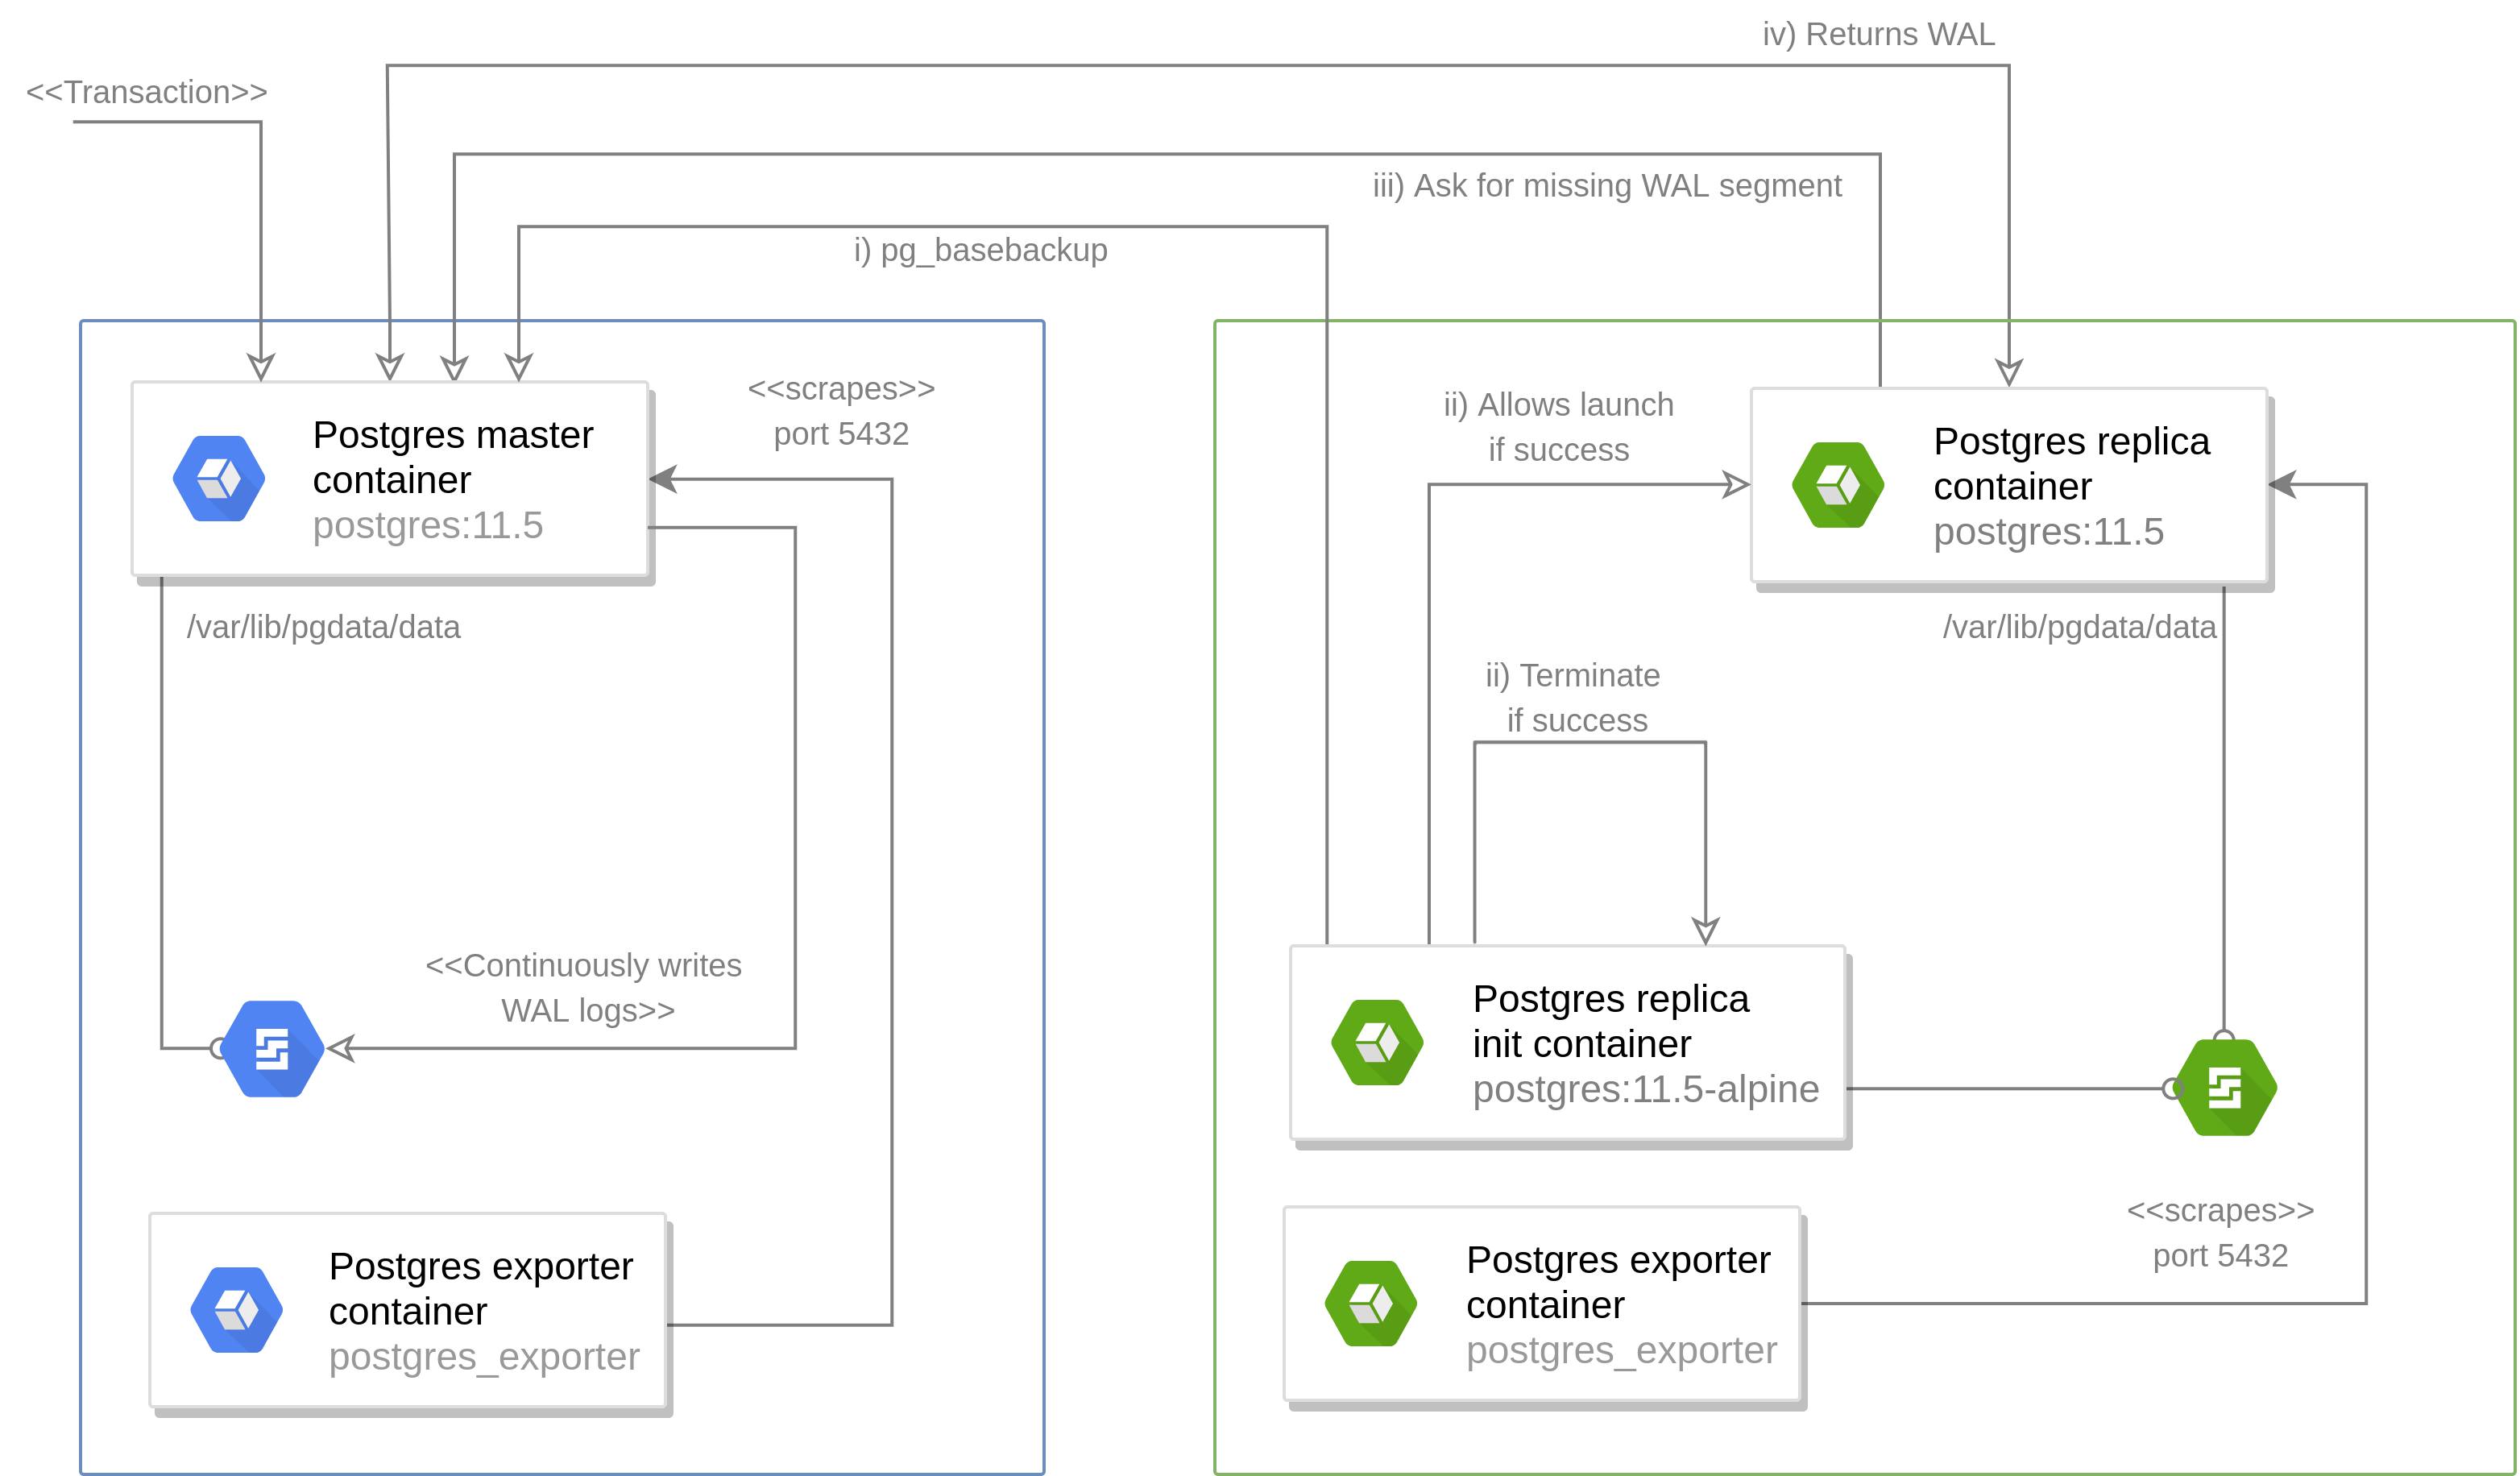
\includegraphics[width=\textwidth]{vulas_postgres.png}
    \caption{Postgres master slave replication in k8s}
    \label{fig:vulas_master_slave}
\end{figure}


\vspace{3mm}
During this initialization and the course of its entire lifetime, the following interaction between the master and slaves occurs:

\begin{enumerate}
    \item The master continuously writes transactions to the transaction log (WAL). Once the size of the WAL logs reaches a predefined limit, the log is closed and a new one is created. Due to limits on disk storage, these are rotated once a limit is reached and archived (archival is described in Section (\ref{sec:vulas_db_resilience})).
    \item The replica nodes frequently queries the master to ask for the most recent WAL segment which it does have and keeps track of the replication lag.
    \item The master sends the most recent WAL segments to the slave, thus ensuring replication and the transactions are committed to the slaves (Insert/ update queries).
\end{enumerate}

\vspace{5mm}
\subsubsection{Connection pooling}

\hspace{5mm} The replication method used (see Section (\ref{sec:vulas_db_replication})) presents one main downside: \textbf{the read and write streams have to be separate to ensure data consistency}, therefore, writing to a replica node is not permitted. 

This is where \textbf{pgpool} comes in and acts as a buffer to distinguish read from write requests and proxy them accordingly without having to change the application's internal logic. This middle-ware also allows for \textbf{Connection pooling} (reducing connection overhead by reusing connections with the same properties), \textbf{Replication} (distinguish between read and write request by analyzing the query), \textbf{Load balancing} (distributing queries between multiple database instances) as well as \textbf{In Memory Query Cache} (increases speed of some requests by storing the SELECT statement result in memory). However, it also comes with overhead costs of its own, querying the database directly would certainly be faster than through any given "proxy".

Therefore, the ensuing benchmark has been done in order to determine whether or not pooling the database connection is beneficial performance wise. 

\vspace{3mm}
\textbf{Benchmarking the database cluster} \label{sec:connection_pool_bench}

\textbf{Reproduction steps}:
\begin{itemize}
    \item Create the database cluster on SAP's Converged Cloud based on three machines, each mounting a $400GB$ PVC provisioned by Openstack Cinder:
    \begin{itemize}
        \item 1 $\times$ 24560MB RAM, 24 VCPU, 64GB disk hosting the master database
        \item 2 $\times$ 16368MB RAM, 16 VCPU, 64GB disk hosting the replicas
    \end{itemize}
    \item Use the previous machines as a node pool for running k8s (version 1.15.2) and a 16GiB, 8vCPUs machine from which to run the benchmarking tool.
    \item Load the production database:
    \begin{itemize}
        \item Total size: 354 GB
        \item Tuples inserted: 412369404
        \item Amount of tables: 30
    \end{itemize}
    \item Run the \textbf{pgbench} tool as a k8s scheduled job within the cluster (on a distinct node from databases) with the following specs (Scaling factor: 1, Query mode: simple, Number of clients: 80, Number of threads: 8, Script: sample of read queries (with varying complexity) representative of the overall population of queries to the real life work load).
\end{itemize}

\textbf{Test cases}:
\begin{itemize}
    \item Master direct: pgbench runs directly against the master node with nclients concurrent clients. This would simulate the 'old' setup but with replication added on which would slightly tax performance.
    \item Slave direct: pgbench runs directly against the slave service (with two exact endpoints). This would be the most optimal situation since pgbench clients can query both databases and thus reduce the response time on both. (Purely hypothetical as test cases only touch read-only queries)
    \item Single pgpool instance: pgbench runs against pgpool connected to one master node and to slaves.
    \item Multiple pgpool instances (2,3,4): pgbench runs against pgpool-service connected to 3 pgpool non clustered instances.
\end{itemize}

\vspace{3mm}
\textbf{Results}

\hspace{5mm} The previous reproduction steps yield the truncated results seen in Table (\ref{tab:vulas_tps}). Clustering pgpool increases postgres's performance drastically when it comes to more complex transactions. This is possibly due to the inbuilt load balancing provided by both service layers (pgpool-service) as well as pgpool load balancing mechanism. This comes at a lower performance for simple requests as the constant shifting and handshakes required makes simple queries unviable (sometimes with 300$\%$ average latencies than other methods).


\vspace{3mm}
\begin{table}[h]
\begin{adjustwidth}{-.5in}{-.5in}  
\begin{center}
\begin{tabular}{|l|l|l|l|l|}
\hline
                                                                      & \begin{tabular}[c]{@{}l@{}}tps with handshake \\ difference from \\ optimal setup (tps)\end{tabular} & \begin{tabular}[c]{@{}l@{}}tps with handshake \\ difference from \\ optimal setup \\ (ratio over \\ slave direct)\end{tabular} & \begin{tabular}[c]{@{}l@{}}tps w/o handshake \\ difference from \\ optimal setup (tps)\end{tabular} & \begin{tabular}[c]{@{}l@{}}tps w/o handshake \\ difference from \\ optimal setup \\ (ratio over \\ slave direct)\end{tabular} \\ \hline
\textbf{\begin{tabular}[c]{@{}l@{}}Slave \\ Direct\end{tabular}}      & + 0.00                                                                                               & 0\%                                                                                                                            & + 0.00                                                                                              & 0\%                                                                                                                           \\ \hline
\textbf{\begin{tabular}[c]{@{}l@{}}Master \\ Direct\end{tabular}}     & - 1.279175                                                                                           & - 10.6\%                                                                                                                       & - 1.279145                                                                                          & - 10.6\%                                                                                                                      \\ \hline
\textbf{Pgpool}                                                       & - 2.478072                                                                                           & - 20.6\%                                                                                                                       & - 2.45631                                                                                           & - 20.4\%                                                                                                                      \\ \hline
\textbf{\begin{tabular}[c]{@{}l@{}}Pgpool \\ cluster(3)\end{tabular}} & + 1.251716                                                                                           & + 10.4\%                                                                                                                       & + 1.2518890                                                                                         & +10.42\%                                                                                                                      \\ \hline
\end{tabular}
\end{center}
\end{adjustwidth}
\caption{Transactions per seconds per test case}
\label{tab:vulas_tps}
\end{table}

\vspace{3mm}
Similarly, from the pgpool test case, using the amount of replicas as the variable yields results presented in Figure (\ref{fig:vulas_db_pgpool_replicas}). This confirms that having the amount of pgpool replicas being equal to the sum of the amount of master and slave replicas is the optimal setup to reduce both latency and increase tps. Going overboard with the amount of replicas is also visibly detrimental to the overall system's health.

\begin{figure}[h]
    \centering
    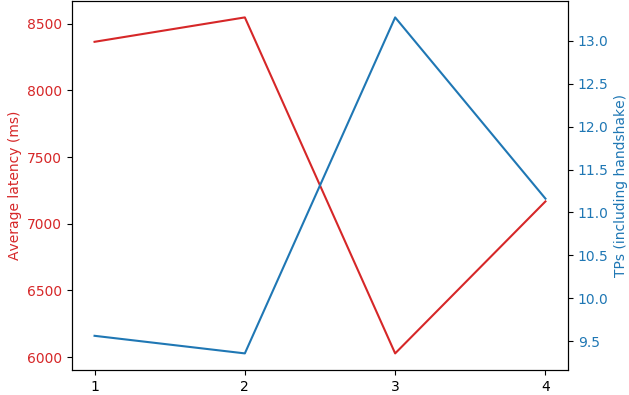
\includegraphics[width=0.8\textwidth]{vulas_pgpool_benchmark.png}
    \caption{Query performance per pgpool replicas}
    \label{fig:vulas_db_pgpool_replicas}
\end{figure}

\subsubsection{Persistence and Resilience} \label{sec:vulas_db_resilience}

\vspace{-2mm}\hspace{5mm} Data stored in the database are critical and should be stable and resilient to outages. 

With the replication scheme previously described, even if a node containing a database were to go down, the data persists in multiple replicas and can be easily restored. If the master node goes down, the system is temporarily read-only and the replicas take charge as the sole read endpoints. Therefore data resilience to node outage is partially guaranteed. 

On the other hand, network outages can be mitigated using WAL archival in the master node. These incremental backups are vital to allow disconnected nodes to catch up to the replication lag. However, due to the storage limitations and WAL files keep getting generated, the space is bound to be recycled and a replica can no longer use that checkpoint to catch up. The maximum size of WAL logs is therefore of utmost importance and defined by two \textbf{constant} (unable to be changed live) parameters:

\begin{equation}
    wal\_size = max\_wal\_size \times wal\_keep\_segments
\end{equation}

The deployment can therefore handle all network outages during which the amount of transaction logs written do not surpass $wal\_size$. If this time frame is exceeded, manual intervention is required to delete the PVC, PV and Pod and force the recreation of a new replica (as previously described in Figure (\ref{fig:vulas_master_slave})). 

In order to further decrease downtime when confronted to this scenario, Openstack's snapshot functionality can be leveraged to periodically store a copy of the volume mounted on the master node. This is useful in two scenarios:
\begin{itemize}
    \item when the master node is corrupted in order to quickly spin up the system
    \item when replicas have fallen too far behind, the latest snapshot can be mounted to a temporary pod to be demoted (cleaning up the master configuration and mounting the slave one) and then to a newly spun up slave pod. This requires that the snapshot interval must be strictly lower than the period to accumulated an archive of $wal\_size$.
\end{itemize} 

\subsubsection{Release and database change}

\hspace{5mm} Over the development cycle of the vulnerability-assessment-tool, the underlying data model is bound to change and this shift has to be seamlessly applied to the PostgreSQL database. All modules of applications destined to communicate with the database uses a object-relational mapping named \textbf{Hibernate} which translates an object oriented data structure into a set of tables and rows (traditional SQL). Along with \textbf{Flyway}, used for creating and applying incremental schema migration scripts, this creates a continuous delivery pipeline reflecting changes in the application data model in the database. 

In edge cases, this migration can fail and corrupt all production critical data so a method to revert the damage is mandatory to maintain this system. 

\textbf{Proposition}

The k8s proposition (summarized by Figure (\ref{fig:vulas_db_change})) attempts to address the rollback issue whilst minimising the downtime and maintaining a viable staging environment. An utility, implemented in Golang, has been developed to perform the following actions:

\begin{enumerate}
    \item Fetch the amount of replicas of the postgres slave stateful set in the given namespace and cluster (at least 2 replicas are required to have a no downtime upgrade).
    \item Scale down one replica from the slave statefulset and store the name of PVC mounted by this replica (which will persist after the scale down operation). This effectively makes an instant k8s native snapshot of the master database whilst keeping the old deployment completely functional. 
    \item Create an ephemeral job that mounts the previous orphaned PVC and promotes the slave to master (by deleting the recovey.conf file).
    \item Spin up a new release (core chart) with a new release name with the master mounting the previously promoted volume. The new rest-backend (Flyway has its own data race management mechanism which only permit a single instance to perform the migration) then applies the schema changes without threatening data loss (the old release still coexisting).
    \item Once the administrator validates the changes in the staging release, reroute the load-balancer/ingress controller to serve the staging release and remove the old one, effectively promoting the staging area to the production one. 
\end{enumerate}

\begin{figure}[!h]
    \centering
    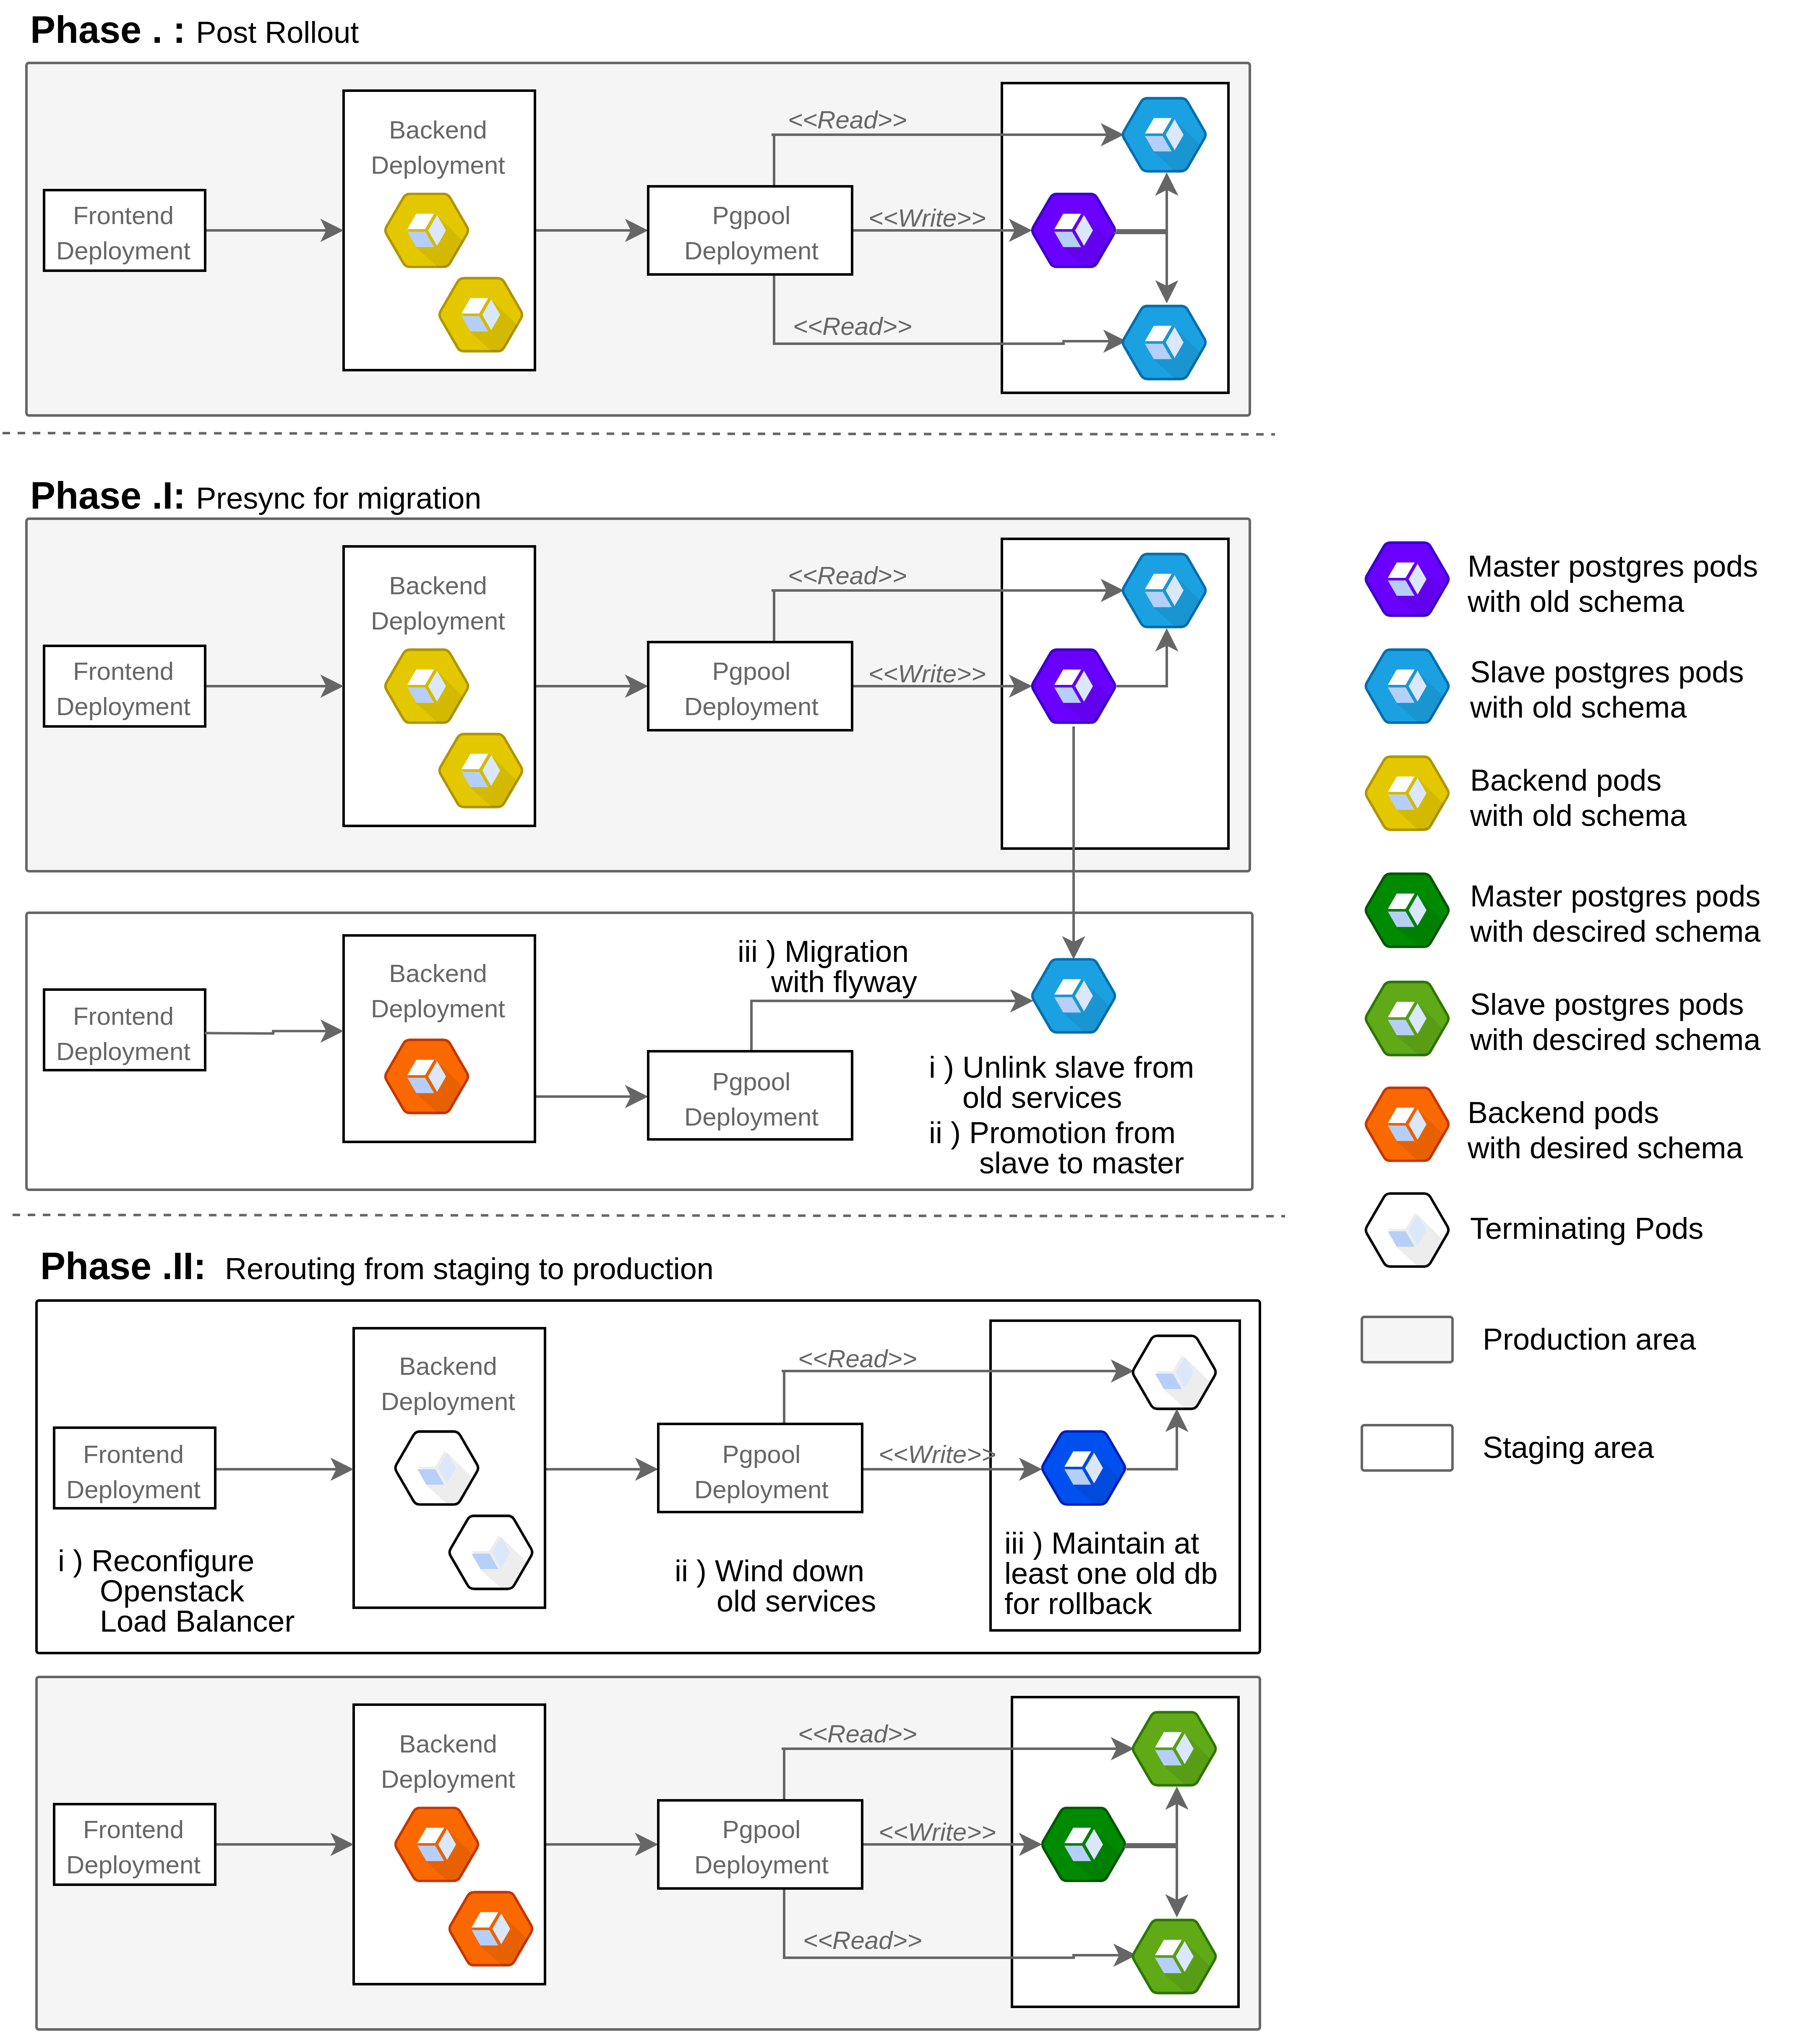
\includegraphics[width=0.91\textwidth]{vulas_database_change.png}
    \caption{Proposed schema change migration}
    \label{fig:vulas_db_change}
\end{figure}

\newpage
In order for two environments (staging and production) to coexist without conflicts, every service selector has to be specific to the release and the labelling scheme must be strictly implemented (with all object having the appropriate release name as a label).

This method guarantees a near 0 down time upgrade with the only time-consuming step being the populating of the newly spun up slave replicas which takes around 5-6 minutes for a data load of around 350GB. During this step, the old release will still be completely functional but any write operations won't be translated to the new deployment. When it comes to the rerouting, it could be done via LoadBalancer rerouting (which directly depends on the cloud provider implementation) or by modifying ingresses selectors and live ingress controller reloading for an instant reload. 

\vspace{5mm} 
\subsection{Core component}

\hspace{5mm} Due to the sheer amount of components that constitute the core architecture of the tool, this section will go over the overarching themes and decisions that led to the creation of the vulnerability-assessment-tool-core helm chart.

\subsubsection{Resource allocation}

\hspace{5mm} Defining resource demands for each container is mandatory in order to maintain a secure k8s deployment. The range defined on CPU and memory usage being a soft enforcement, once the limit is reached, the container is throttled and not killed, thus, ensuring both the vertical scalability of the pod and slight buffers against DDOS attacks. 

The lack of a proper toolkit and data of resource usage is one of the main roadblocks in defining proper resource usages. Therefore, one has to use previous observations of the system along with general knowledge about the application's language and frameworks used to issue a meaningful resource usage limit range. 

\vspace{3mm}
\textbf{Java and OpenJDK8}

All components of the architecture are implemented in Java, specifically OpenJDK-8 which, either through fault of implementation or design flaw, more often than not has issues with memory leaks. It is therefore wise to allocate quite a bit of memory for these containers. 

At the same time, container support for Java 8 is quite poor. The JVM fails to perceive the system's resources from within the allocated docker cgroup and assumes that it is allocated the entirety of the host's resources.  It sets — by default — the maximum heap size to 1/4 of system memory and sets some thread pools size (for example for GC) to the number of physical cores. Consequently, containers often go over resource limits and lead to them being OOM (out of memory) killed. 

The \textbf{openjdk:8u212} image resolves this issue by integrating the back-ported Docker support. It is therefore mandatory to switch the base image to a subsequent tag. Further fine tuning can be done via environment flags such as $-XX:InitialRAMPercentage$ which require an in heap depth profiling of each container which we'll no explore further. 

\textbf{Frameworks and Workload}

Thanks to data collected by the "old" monitoring stack, average and peak CPU and memory usage are available and can be extrapolated to fit with the k8s deployment. 

\subsubsection{Persistent caches}

\hspace{5mm} Some applications benefit greatly from having a shared cache between different replicas. For instance, the rest-lib-utils often clones git repositories locally in a cache directory, an operation which should not be done by every container. This cache directory can then be shared between replicas to avoid the redundant operations. However as described in Section (\ref{sec:k8s_volumes}) ReadWriteMany volumes are not offered by any cloud provider and should be self provisioned. 

Before attempting to implement any shared filesystem solution, it is important to establish whether or not the computation cost and communication cost between nodes is lower than the cost of running the operation redundantly on each node. Although the theoretical approach of estimating the complexity of the previously mentioned costs is more sound. In practice, it is impossible to establish such a measure and more viable to run a benchmark of both deployments. The proposed benchmark consists of running the patch-lib-analyzer cronjob against the rest-lib-utils containers to load and find vulnerable constructs for 1024 CVEs. Due to time constraints, this benchmark is not run multiple times. On the single sample observed, the shared file system solution (NFS) yield an approximately $12\%$ lower execution time than its counterpart. With this positive result, a couple options for provisioning ReadWriteMany volumes are possible;

\subsubsubsection{NFS (Network File System)}

\vspace{-5mm}\hspace{5mm} NFS is a distributed file system protocol which allows remote hosts to mount file systems over a network and interact with those file systems as though they are mounted locally. NFSv2 and NFSv3 can both use TCP or UDP running over an IP Network. Although stateless UDP connection translate into better performance on clean, non-congested networks (often the case in intra-cluster network) thanks to lower protocol overhead, using TCP increase reliability and offer better error detection as to not overload the network. Going forward with using TCP, the protocol (v2 and v3) uses RPC (remote protocol calls) to request a service from the host machine over the network and therefore require the \textbf{portmapper} (utility to map RPC services to the ports they are listening on), the \textbf{mountd} (daemon implementing the NFS MOUNT protocol) ports to be exposed as well as the \textbf{nfs protocol} ports to be exposed to the network. 

In the case of rest-lib-utils component, the cache directory can be served over a network, allowing concurrent access from multiple containers. Deployment an NFS provisioner in a k8s context can be done either by leveraging k8s functionalities or by leveraging the underlying Cloud Provider functionalities.

A k8s native NFS provisioner would require an nfs-server deployment (with a single replica) mounting a PVC backed by a PV provisioned by the default provisioner which is served through a clusterIP service exposing the ports previously mentioned (see Figure (\ref{fig:vulas_nfs}.a)). 

The cloud provider based deployment is similar, although the NFS service is an ExternalName pointing to the hosted NFS server. However, in most providers, the cluster network is not within the same subnet as the NFS one, therefore a VPC bridge (with the appropriate networking rules) is required for this setup to properly function.

\vspace{2mm}
\begin{figure}[h]
    \centering
    \subfloat[k8s native]{{\includegraphics[width=0.44\textwidth]{vulas_nfs_server_native.png}}}
    \hspace{2mm}\vrule\hspace{2mm}
    \subfloat[cloud provider]{{\includegraphics[width=0.5\textwidth]{vulas_nfs_server_hosted.png}}}
    \caption{NFS server deployment scenarios}
    \label{fig:vulas_nfs}
\end{figure}

\vspace{5mm}
\textbf{CIFS (Common Internet File System)}

This protocol is chattier NFS and is more adapted to mixed client environments (Windows and Unix hosts). Since the cluster is made up of Unix only clients, this option is not chosen.

\subsubsubsection{Ceph Storage Cluster}

\vspace{-5mm}\hspace{5mm} Ceph is a distributed filesystem which unlike NFS also defines how data is stored and served. Deploying the Ceph Storage cluster requires the following components:
\begin{itemize}
    \item \textbf{Monitors}: component that maintains the map of the cluster state.
    \item \textbf{Managers}: keeps track of runtime metrics
    \item \textbf{Ceph OSDs}: object storage daemons that handle data storage, replication, recovery, re-balancing, etc...
    \item \textbf{MSDs}: metadata storage for the filesystem 
\end{itemize}

Due to the complexity of its installation and numerous components, Ceph is usually installed with Rook (an operator meant to simplify storage orchestration in k8s) to create a provisioner for ReadWriteMany volumes. Through the Rook abstraction, an application can then issue a ReadWriteMany volume claim with the appropriate storage class (Block Storage in this case) and the Ceph Storage Cluster would be the provisioner backing said claim.

Despite the scalability and abstraction provided by this architecture, the cache data stored is not critical enough to warrant replication and the overhead cost of this system would overshadow the benefits of the cache. Therefore, cache data storage would be done using NFS.

\subsection{Monitoring and Logging infrastructure}

\hspace{5mm} Having a good log and monitoring infrastructure becomes a key feature that allows sysadmins, support teams, and even developers to be more prepared to face these possible operational problems and address problems in the code base more efficiently. 

\subsubsection{Scalable application monitoring with Prometheus}

\hspace{5mm} Metrics, unlike logs, are a measurement at a point in time for the system collected at a fixed-time interval and not collected per event. As such, it is the fundamental building block of application monitoring allowing for an objective overview of the health of the given system. 

\textbf{Prometheus} is the metrics and alerting server with the highest amount of adoption and integration for k8s which is going to be used in our case. It relies on a set of exporters (components to export specific metrics) to run on the desired instance and send it back to the server to be aggregated. After a brief discussion about the required metrics, the following exporters are included in the deployment:
\begin{itemize}
    \item \textbf{cadvisor}: provides information regarding the resource usage and performance of containers. It should be run as a daemon set on each node as it only fetches data on the node on which it's hosted and extremely lightweight (20MB). A couple major downsides of this component are that it offers an unwanted mandatory UI that consume resources and requires root privilege (reading from /sys/ and /rootfs/) to function.
    
    \item \textbf{kube-state-metrics}: exposes k8s cluster level metrics such as allocatable cpus per node. Only a single replica is required because it communicates with the k8s API.
    
    \item \textbf{postgres-exporter}: publish metrics about the PostgreSQL database (such as replication lag, most used queries, etc...). This component is integrated as sidecar container to the postgresql database container.
    
    \item \textbf{nginx-ingress-controller}: metrics endpoint already available in the ingress controller deployment which allows for monitoring request latency and HTTP responses.
\end{itemize}

It is important to note that the monitoring architecture (see Figure (\ref{fig:vulas_monitoring})) has not been altered from the docker-compose based deployment albeit with the addition of cluster metrics. 

\begin{figure}[h]
    \centering
    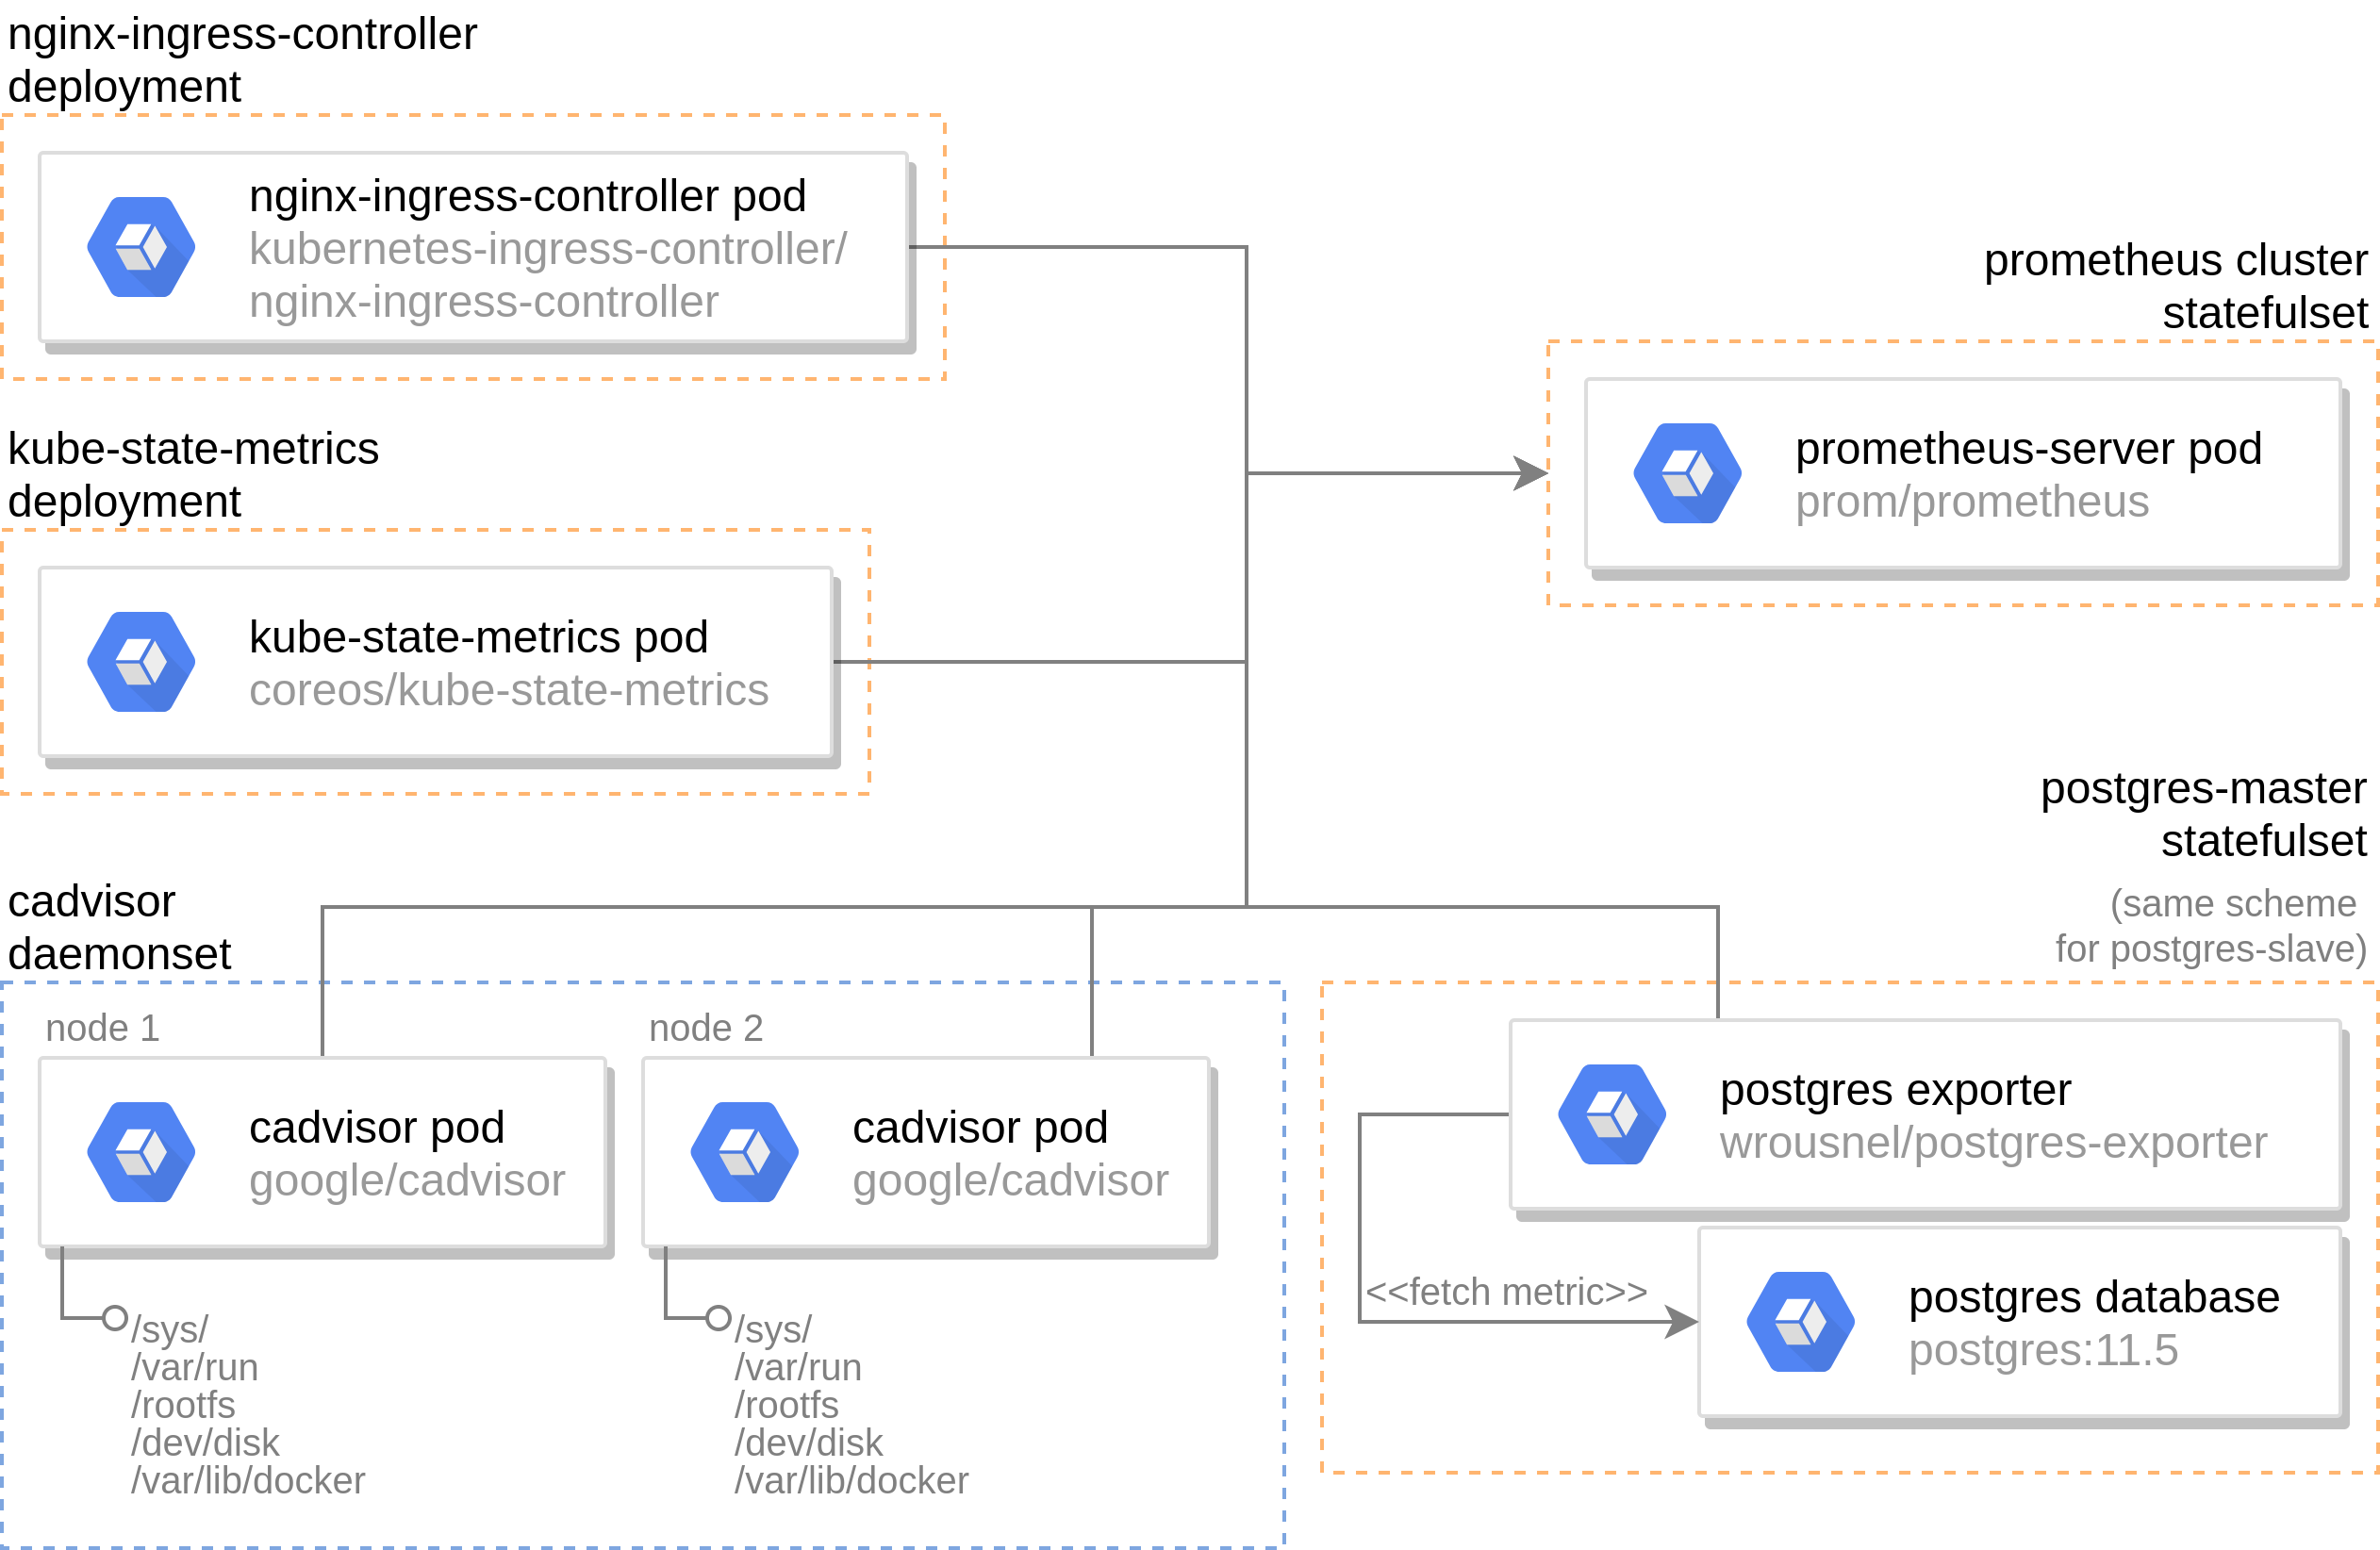
\includegraphics[width=0.9\textwidth]{vulas_monitoring.png}
    \caption{Simplified k8s deployment of the monitoring infrastructure}
    \label{fig:vulas_monitoring}
\end{figure}

\subsubsection{Log pipeline implementation}
\hspace{5mm} The traditional solution to this question is the \textbf{ELK} stack (Elasticsearch, Logstash, Kibana) which it composed of four components; \textbf{Filebeat} which ships logs from the host machine to \textbf{Logstash}, which aggregates and filters them before loading them into \textbf{Elasticsearch}, a database which can be fed into \textbf{Kibana} to create meaningful visualizations and time series analysis (see Figure (\ref{fig:vulas_logging_stack}.a)). 

\begin{figure}[h]
    \centering
    \subfloat[ELK stack]{{\includegraphics[width=0.44\textwidth]{vulas_elk_logging.png} }}%
    \quad
    \subfloat[EFK stack]{{\includegraphics[width=0.44\textwidth]{vulas_efk_logging.png} }}% 
    \caption{Logging deployment}
    \label{fig:vulas_logging_stack}
\end{figure}

Although this solution is conventional for docker-compose based architecture, it can be problematic in the k8s context because of \textbf{Size}. Filebeat has to be run as a daemonset and thus a container must be present in all machines of the cluster. The filebeat container has a significant footprint (around 100MB, due to it being in Java and requiring the corresponding JVM) and can in no way be considered lightweight.

The \textbf{EFK} stack is chosen because it mitigates this issue, by replacing both Logstash and Filebeat by Fluentbit, a lightweight (20MB) log shipper written in C that doubles as a filter which creates a pipeline from the host machine directly into Elasticsearch (see Figure (\ref{fig:vulas_logging_stack}.b)). 


\subsubsection{Metrics and logs visualization}

For visualizing metrics, Grafana is an open source analytics and monitoring solution for every database which is perfectly adapted to creating meaningful dashboards for prometheus metrics. The large community behind the project has done the hard work of creating dashboards for all use cases which can be imported as a JSON. Therefore the work in creating a meaning visualization adapted for our use case is just a matter of importing this file and modifying some metric names which are prone to change over different versions and release of the exporters.

When it comes to logging, in agreement with the vulnerability-assessment-tool team, a Kibana dashboard is not within the scope of this internship. Nonetheless, live tailing logs is a mandatory requirement. The centralized log infrastructure proposed above is not real time so a workaround has to be devised. Unlike a non cloud deployment, in a k8s environment, a container can be running on a multitude of different nodes and the workload can be divided to different containers. Due to this complexity, there are currently no viable infrastructure based solutions to this demand. 

Shifting the scope of the search to a more contributor/developer side solution yielded \textbf{stern}\footnote{source: https://github.com/wercker/stern}, a CLI tool written in Golang that uses the kubectl CLI and a set of simple arguments to filter out the appropriate logs. As is the case with a lot of libraries, the code design is not thought out for integrating in other Golang projects so we decided to create a Bash wrapper script which fills in the appropriate arguments for the desired containers.

\subsection{Support stack}

\hspace{5mm} The previous components need to be served on the Internet at given set of endpoints. Initially, this task was performed by HAProxy, a high availability load balancer for high traffic websites. However, due to its lack of caching functionality, the current implementation tunnels certain connection through an NGINX deployment serving the content and caching based on a parameters passed through the query (a bool indicating whether to cache and another one indicating its validity). This redundance of web servers lead to higher overhead cost and the cache logic being relegated to the application. 

It its also important to note that in a k8s context, the internal IPs of the machines hosting the web servers are dynamic. As such, the traditional static routing configuration often seen in web servers are inapplicable. \textbf{Ingresses} are k8s native objects meant to address these issues (see Section (\ref{sec:ingress})). Backed by Ingress Controllers, HTTP and HTTPS routes from outside the cluster can be redirected to internal services according to a set of defined rules. 

The NGINX Ingress Controller\footnote{This refers to the ingress controller developped by the Kubernetes dev team and not NGINX's solution for ingress controllers. source: https://github.com/kubernetes/ingress-nginx} has been chosen as the entrypoint to the system to tackle the aforementioned problems with caching and dynamic configuration (see Figure (\ref{fig:vulas_admin})). By utilizing NGINX's feature for caching content, the \textit{X-Accel-Expires} Header can be changed in the application's AJAX query to control both whether to cache the content and its expiry date. For persisting the cache between different replicas of the ingress controller, each pod of the devised statefulset mounts the same NFS on the same cache path. Other solutions such as using a Redis or Memcached cluster as a cache storage are eliminated for its high overhead cost. 

\begin{figure}[h]
    \centering
    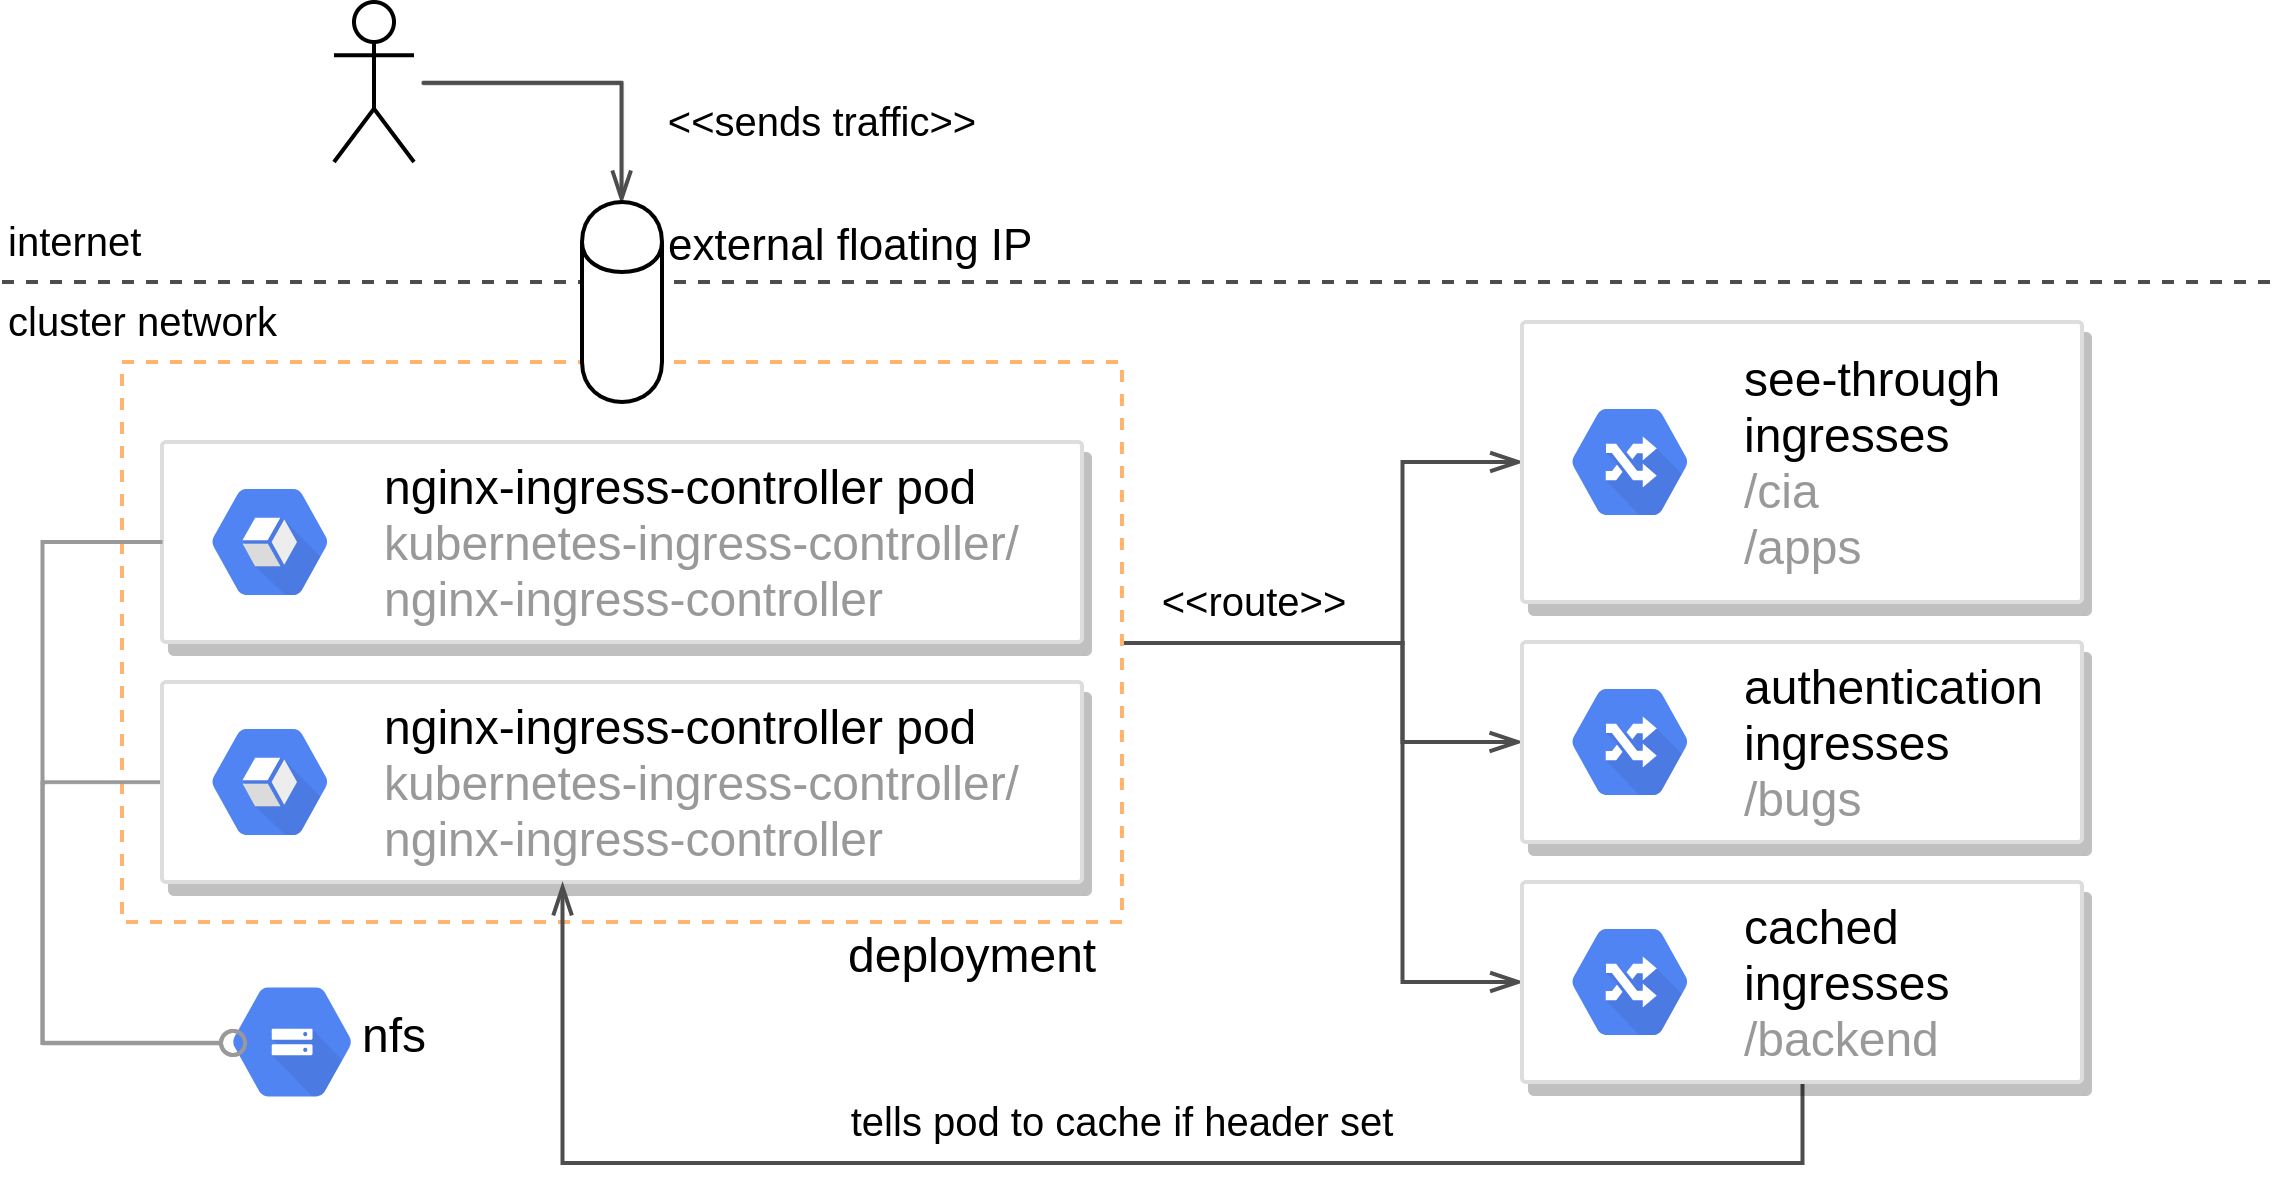
\includegraphics[width=0.8\textwidth]{vulas_admin.png}
    \caption{Simplified traffic schema using the NGINX Ingress Controller}
    \label{fig:vulas_admin}
\end{figure}

In order to serve the contents through a secure connection, an SSL certificate should be added to the nginx-ingress-controller through a config map. This operation is manual and could be automated by using cert-manager\footnote{source: https://github.com/jetstack/cert-manager} to manage and certificate cycling but can't be used due to high overhead costs.

\subsection{Security and delivery  considerations}

\hspace{5mm} Securing a deployment in a k8s environment cannot be restricted solely to k8s and has to extend to multiple context; starting from the application itself, to the container wrapping it, to the pod abstraction said container, to the communication between said pod and even up to the orchestration software configuration behind it.

\subsubsection{Application tightening}

\hspace{5mm} Applying static and dynamic code analysis tool before releases is a mandatory stage in securing the application. A static code analysis tool examines the software code (as source code, intermediate code, or executable) without executing it with specific inputs. 

For static analysis, \textbf{Spotbugs} is used in order to find bug patterns in the Java code base. Possible bugs found are categorized in a couple of categories:
\begin{itemize}
    \item BAD\_PRACTICE and STYLE: Violations of recommended and essential coding practice and anomalous coding styles. These issues do not affect security but should be addressed nonetheless in order to maintain the code base's ease of contribution.
    \item CORRECTNESS: Apparent coding mistake resulting in code that was probably not what the developer intended. This category must be examined case by case in order to determine the mitigation required.
    \item MALICIOUS\_CODE and SECURITY: Code vulnerable to attacks and addressing these possible vulnerabilities should be of the highest priority.
    \item PERFORMANCE and MT\_CORRECTNESS: Inefficient code or flawed implementation of threads, locks and volatiles. 
\end{itemize}

\begin{figure}[h]
    \centering
    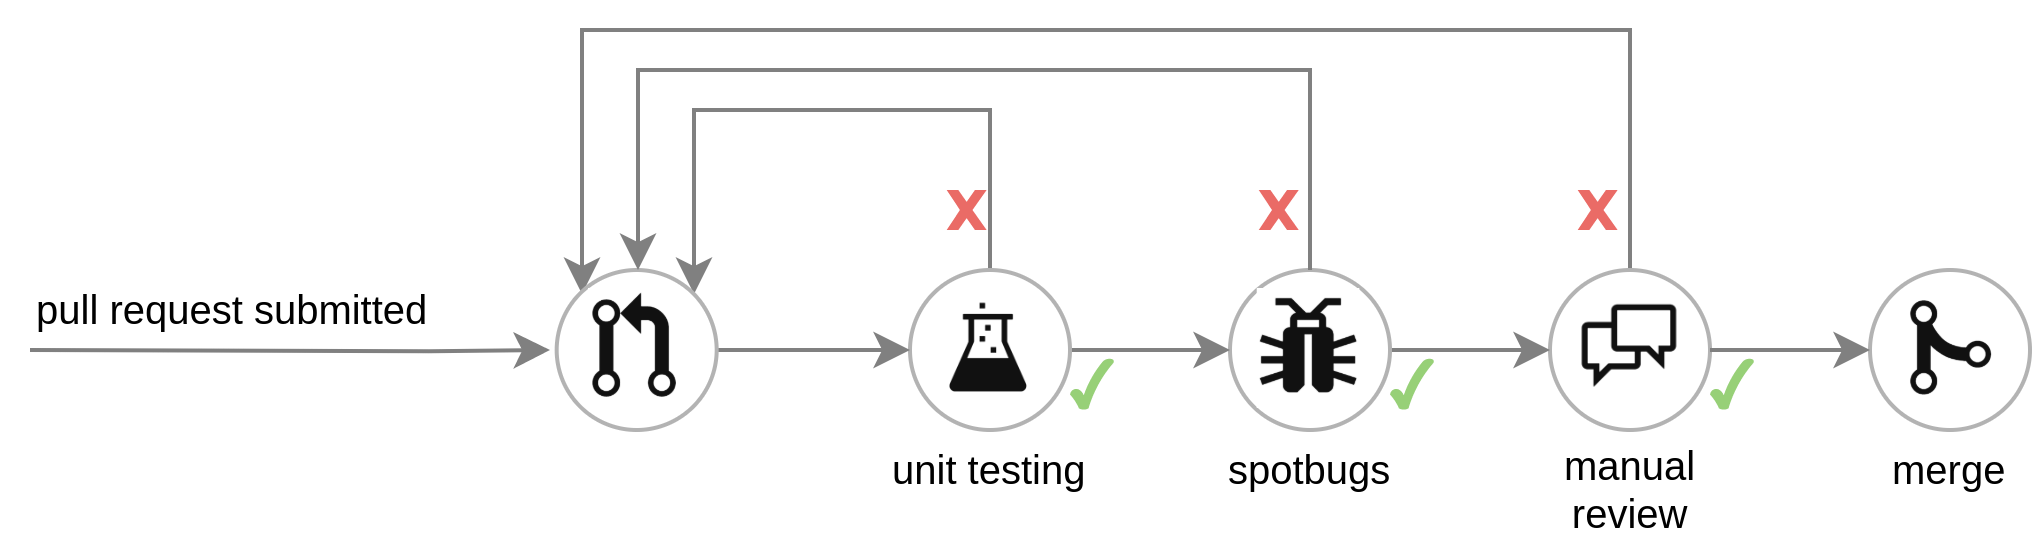
\includegraphics[width=0.9\textwidth]{vulas_spotbugs.png}
    \caption{Simplified contribution pipeline in Travis}
    \label{fig:vulas_spotbugs}
\end{figure}

In order to properly enforce the mitigation of issues found by Spotbugs, a step is added to the pre-existing Travis pipeline that runs the Spotbugs goal and fails if any bugs in the MALICIOUS\_CODE, SECURITY, MT\_CORRECTNESS categories are discovered (see Figure (\ref{fig:vulas_spotbugs})). 

\vspace{3mm}
\subsubsection{Container securing and delivery}

\hspace{5mm} In both production and development environments, the applications are containerized and a couple of major security considerations are to be put into effect.

\textbf{Reducing the Docker image surface}

It is recommended to use minimal base images such as \textbf{alpine} based images over debian based ones. Alpine images are smaller in footprint than traditional GNU/Linux distributions (requiring no more than 8MB for a minimal installation) and offers thinned out and split binary packages which gives better control over the environment installed. This reduction in size and the amount of general system libraries come with a reduction in possible exploit of vulnerabilities in said libraries. At the same time all binaries are compiled as \textbf{Position Independant Executables} (ensuring that the body of machine code function properly no matter its absolute address in the primary memory) with stack smash protection (which in turn limits possible damage afflicted by buffer overflow attacks).

\textbf{Least privileged users}

Docker containers that do not specify its USER defaults to executing the container using the root user. When that namespace is then mapped to the root user in the running container, it means that the container potentially has root access on the Docker host which put the host machine at risk of privilege escalation attacks.

\subsubsubsection{Jib — A dual purpose solution}

\vspace{-5mm}\hspace{5mm} Jib is an open-source software published by Google that that builds optimized Docker for Java applications based on \textbf{distroless} containers. 

Distroless containers, unlike Alpine or other small footprint base images have fundamentally different philosophies and approaches to building containers: whereas the former attempts to trim down a distribution to the limit at which it is sufficient for the app to run, distroless attempts to build the container from the standpoint of what the application needs. From this thought process, the distroless images are bootstrapped by selectively extracting debs (Debian package). For compatibility, apk was not chosen, thus substituting musl (alpine's C standard library of OS's based on the Linux kernel) with glibc (GNU Project's implementation of the C standard library). Distroless containers therefore only contain the application and its runtime dependencies, without any package managers or shells (reducing even further the surface of potential attacks at the cost of harder debugging).

Jib builds itself on the foundations of the distroless base image to build Java applications. Unlike traditional build systems in which a Java application is built as a single image layer with the application JAR, Jib separates the Java application into multiple layers for more granular incremental builds. This increases the speed of image builds drastically, by only changing the layers that have changed to the registry. It also abstracts the packaging process itself as it runs as part of the Maven build without requiring a Dockerfile or a running Docker daemon. 

\begin{figure}[!h]
    \centering
    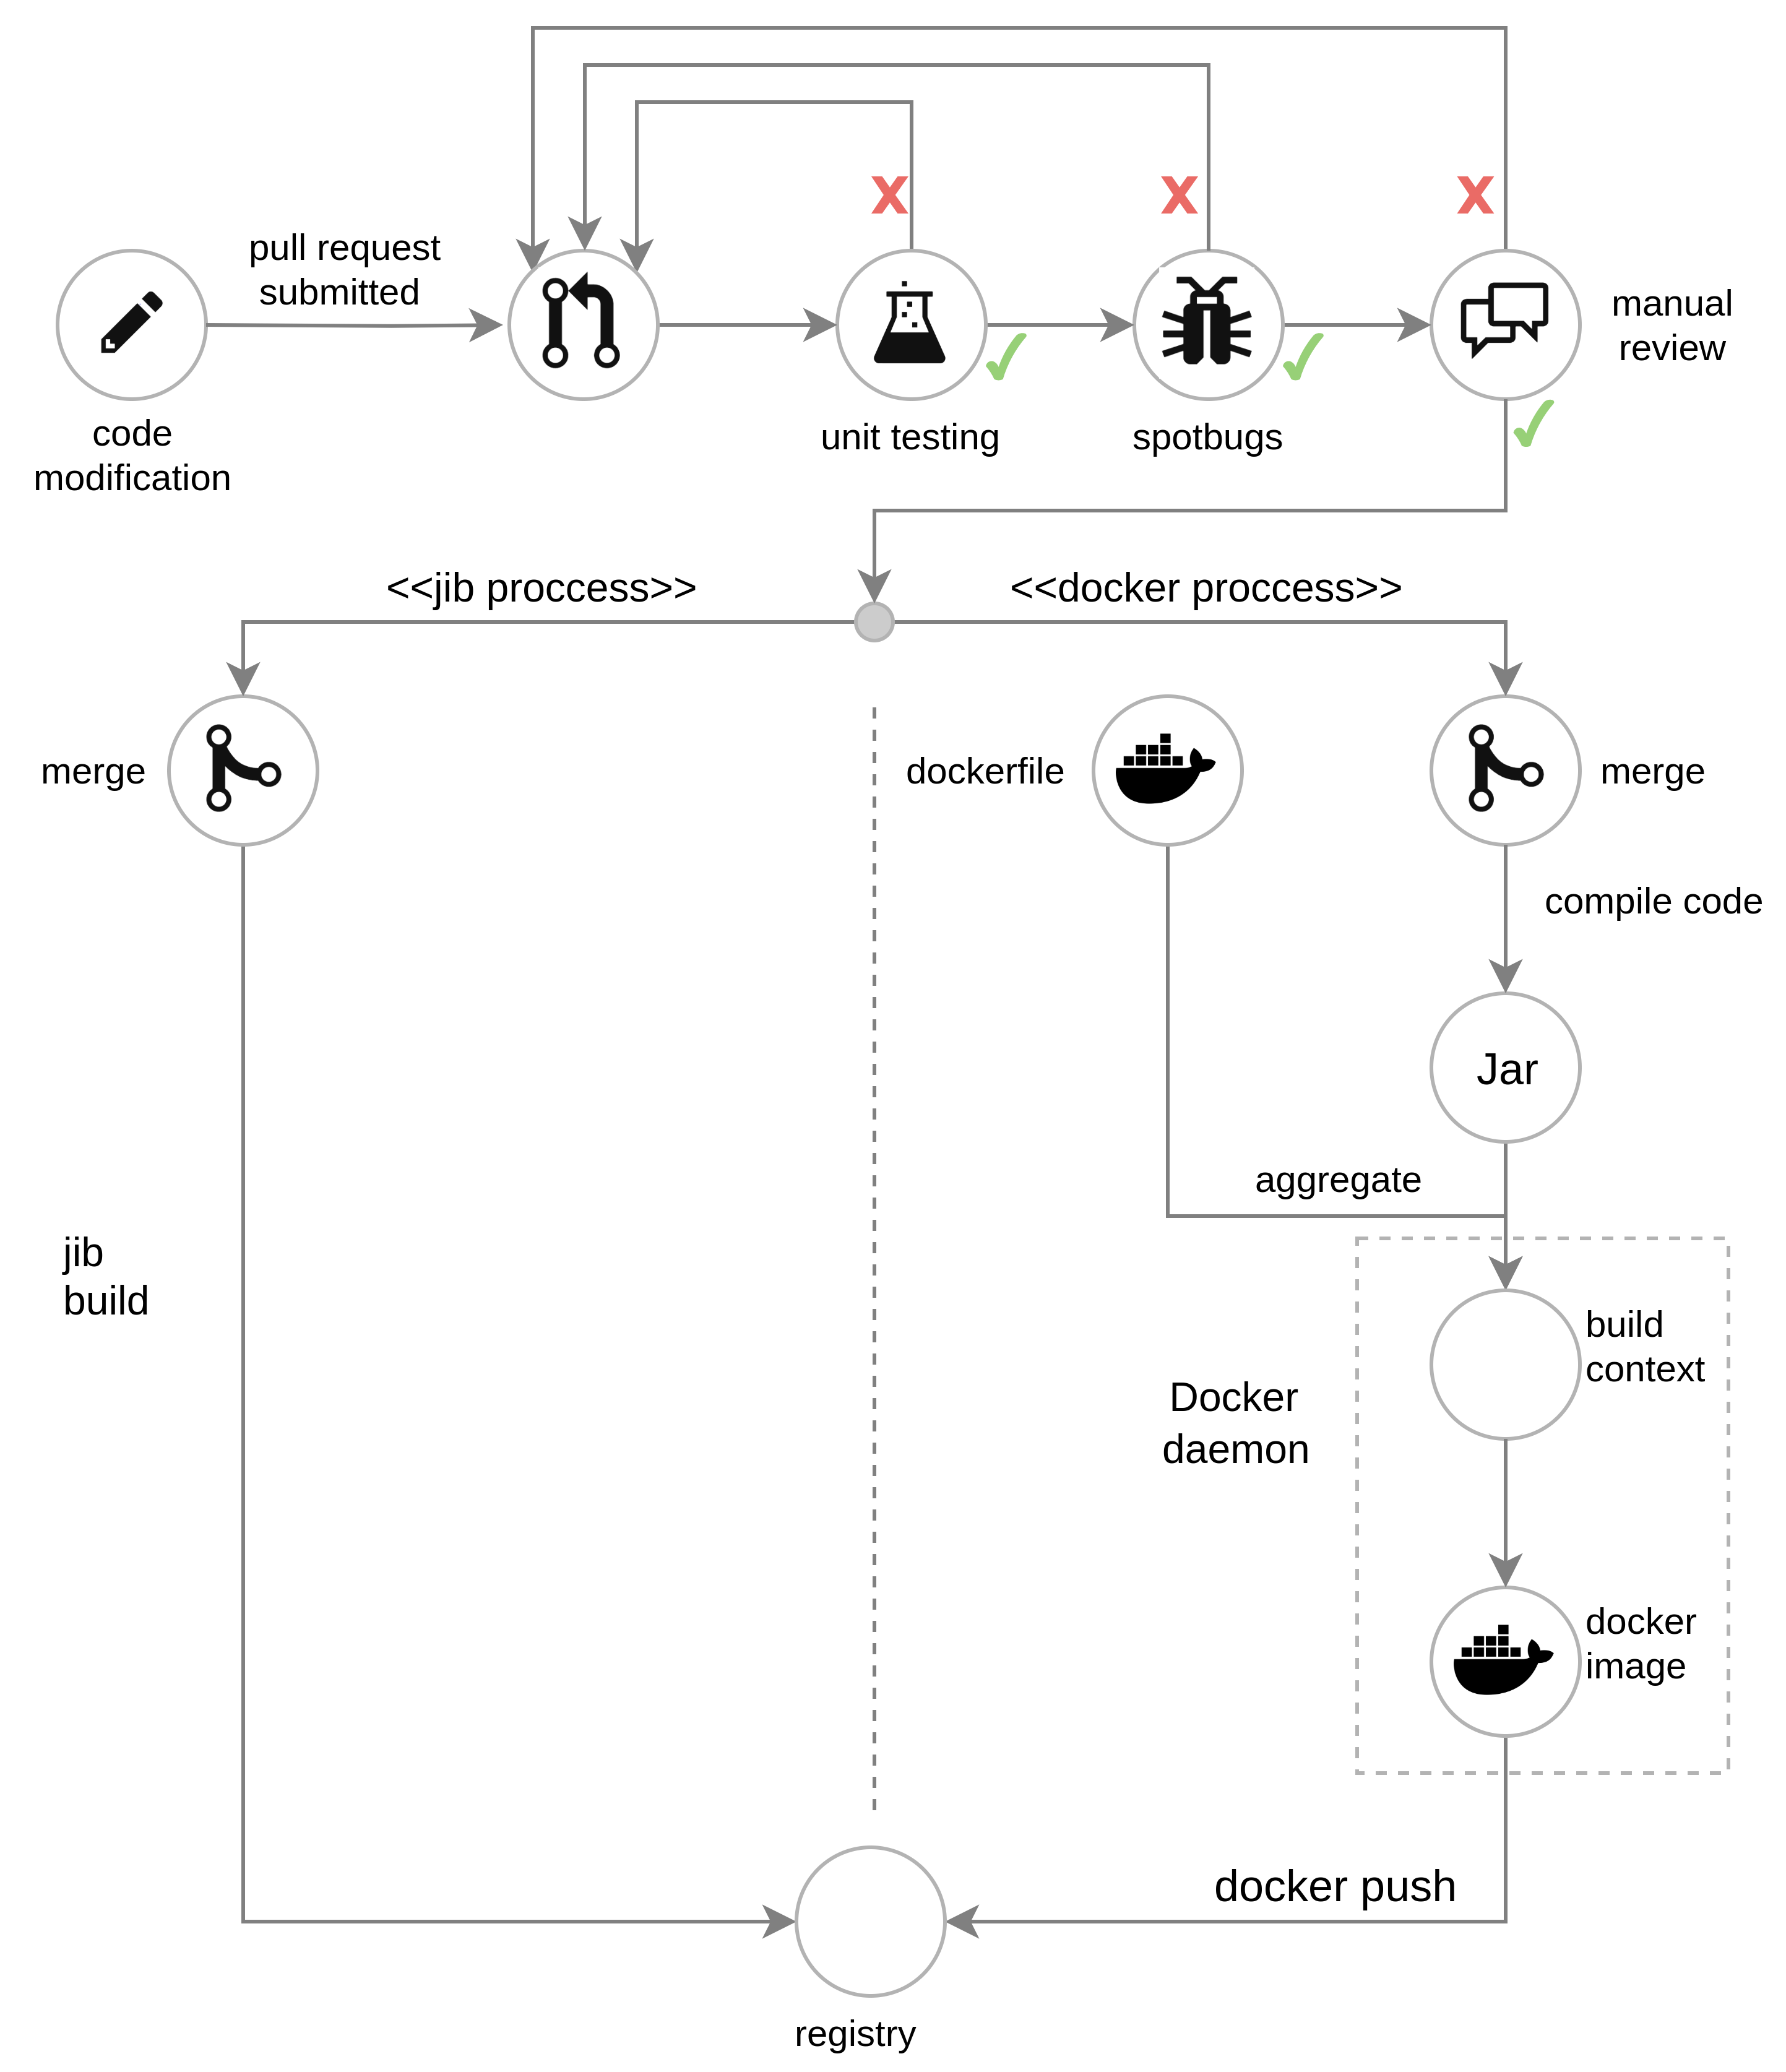
\includegraphics[width=0.8\textwidth]{vulas_jib.png}
    \caption{Deployment pipeline for docker and jib cases}
    \label{fig:vulas_jib}
\end{figure}

The simplification of the deployment (see Figure (\ref{fig:vulas_jib})) process along with the added benefits of a secure container makes it a viable replacement to using docker images in our use case. 

Performance wise, the exploded tar springboot containers built by jib also create observable speedups when it comes to startup time on all spring version to its fat jar counterpart  (see Spring benchmark \cite{SPRINGBENCH}). This performance gain comes at the cost of slightly bigger footprint than alpine based images of around 20-30MB in average. 

\subsubsubsection{Skaffold — Continuous delivery for Kubernetes}

\vspace{-5mm}\hspace{5mm} The previous deployment process using Jib would only update the images published to the registry whilst not triggering any changes in any deployment. Combining the Jib build methods with the Skaffold tool will facilitate the continuous delivery of code changes to the k8s deployment itself. 

\begin{figure}[h]
    \centering
    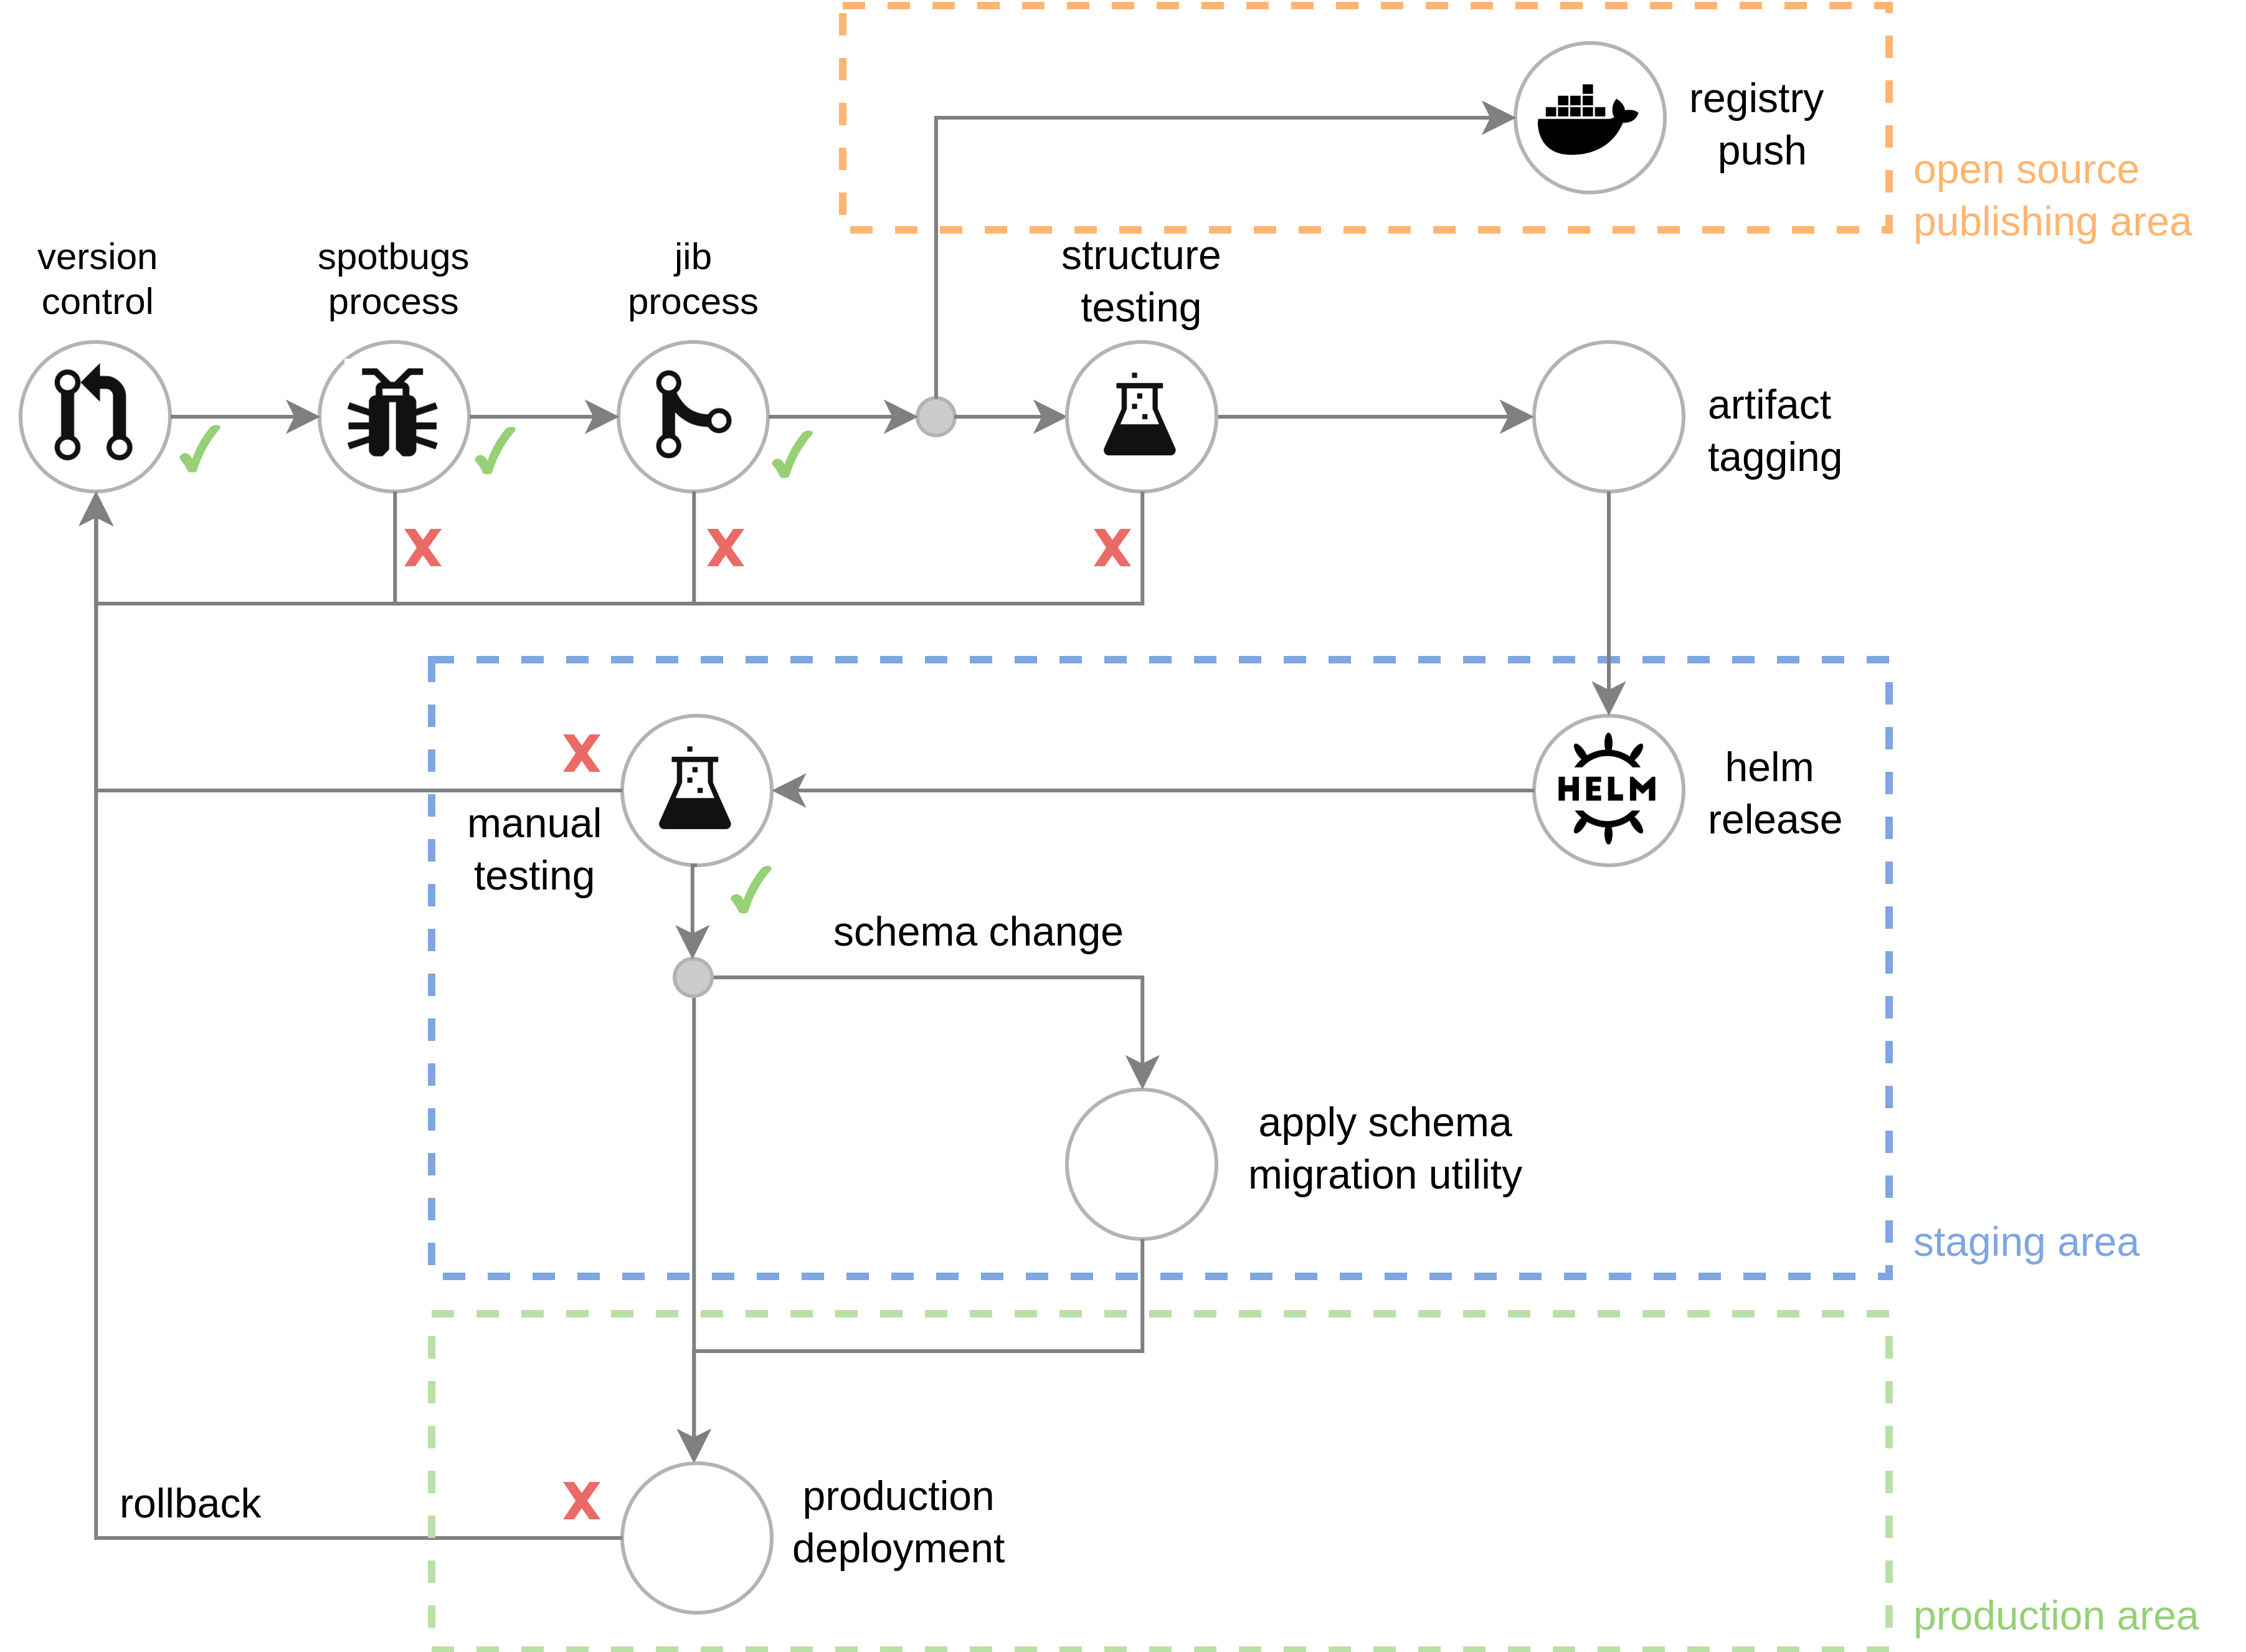
\includegraphics[width=0.9\textwidth]{vulas_skaffold.png}
    \caption{Skaffold deployment process}
    \label{fig:vulas_skaffold}
    \vspace{-3mm}
\end{figure}

Integrating skaffold into the Travis pipeline would allow a hands free rolling update on all containers whose code is affected by the change (see Figure (\ref{fig:vulas_skaffold})). However, despite its integration testing functionality based on \textbf{container-structure-test}, this tool is not mature enough to be applied in a stable production environment and should be delegated to the development environment to provide a direct source code to deployment solution. 

\vspace{3mm}
\subsubsection{Pod hardening}
\subsubsubsection{Pod security context design}

\vspace{-5mm}\hspace{5mm} Pod security contexts are particularly tricky to implement but allow for enforcing privilege and access control settings for a Pod or Container. 

\vspace{3mm}
\textbf{Enforcing UID and GID}

By default, the group and user run in a pod/container will be root(0). Due to security concerns and possible privilege escalations, specifying a different UID and GID constitutes good practice. The nobody user (65534) is the "go to" UID for this task, who in Unix systems has the lowest privileges possible. However, this practice is questionable due to file permission issues as this user is meant for files that must not be accessible by anybody. Keeping a common easy to remember and non conflicting id (over 10000), we can pick 12000 as an UID and GID for all containers.

\vspace{3mm}
\textbf{Granular capabilities attribution}

In order to respect the principle of least privilege, a pod should must be able to access only the information and resources that are necessary for its legitimate purpose. \textbf{Linux capabilities} offer a mechanism through which to satisfy this principle by dividing the privileges traditionally associated with superuser into distinct units. For example, granting a pod the CAP\_CHOWN allows the process to make arbitrary changes to file UIDs and GIDs. It is impossible to create a set of rules for all container use cases but through trial and error, we have managed to establish a minimal set of capabilities required for a container:

\begin{itemize}
    \item CAP\_NET\_ADMIN: allows for performing network-related operations (for instance modify routing tables and binding sockets).
    \item CAP\_DAC\_OVERRIDE: allows for bypassing read, write and execution permission checks (useful for containers that require disk operations).
\end{itemize}

It is important to note that the granularity provided by Linux capabilities is often too large (capabilities are either not sufficient for execution or as permissive as root). AppArmor or SELinux is more adapted for fine-grain pod security context hardening.


\subsubsubsection{Secret administration}

\vspace{-5mm}\hspace{5mm} Solutions for storing and injecting credentials and sensitive information were then examined in order to properly secure the database access. 

\vspace{3mm}
\textbf{Native secret storage}

k8s secrets are objects that store a key value map with the value being base64 encoded and not encrypted. Therefore, committing these values to the source control (in our case git) is not recommended. However, in our case, the potential damages can be nullified because the operational git repository is hosted in the private Github Enterprise at the expense of extra effort required to maintain both an open-source repository and a private one.  

Credentials can also be obfuscated completely from declarations by using Kustomize's secret generators or ignoring production values.yaml files if Helm is used. These "hacks" does not address the issue of having plain text credentials in the repository.  

\vspace{3mm}
\textbf{Hashicorp Vault}

Vault is meant to address the complexities of secret management by centralizing management and access enforcement to secrets and systems based on trusted sources of application and user identity. In the context of k8s, it allows for a pod to use given service account token to dynamically fetch the appropriate secret. These dynamic secrets encrypted both during storage in the Vault database and during transit. Although, the shift to an Identity based access to dynamic encrypted secrets would be perfect from the security point of view. The overhead cost of the Vault deployment cannot be justified in our use case despite the advantages.

% \subsubsection{Network groups and policies implementation}

% \subsubsection{Cluster configuration}

\subsection{Infrastructure provisioning}

\hspace{5mm} It is important to note here that choices regarding the infrastructure cascade from decisions made in the implementation of the core components and the monitoring stack and not vice versa. 

\subsubsection{Kubernetes cluster creation}

\hspace{5mm} Creating the underlying computing and networking resources for a functional k8s cluster can be done in two distinct ways:

\begin{itemize}
    \item \textbf{Manual}: 
    \begin{enumerate}
        \item Create the node pool on which Kubernetes will run
        \item Create networking resources to connect the different nodes in the same subnet
        \item Setup the k8s prerequisites (disable swap on all machines, install docker) via Ansible then the k8s architecture via Ansible while keeping in mind the differences between the master and worker nodes (described in Section (\ref{sec:high})) or with the \textbf{kubespray} tool.
    \end{enumerate}
    \item \textbf{Hosted control plane}: rent the control plane (etcd, metrics server) and define the node pool resources to be automatically provisioned. 
\end{itemize}

The first option allows for a better control of the environment in which the cluster runs at the expense of higher overhead cost (more scripts to manage). The difficulty of creating and maintaining up-to-date and reproducible infrastructure code (even with Ansible) directly violates objectives (\ref{obj:dep_overhead}) and (\ref{obj:dep_reprod}) defined above. The usage of tools such as Ansible also increases the time to spin up an instance drastically, thus, violating goal (\ref{obj:dep_spin}). 

Whereas, the hosted option exchanges that control for a auto-managed cluster with extra services (automated backup of the etcd server, metrics, monitoring and logging stack often external to the cluster itself). As it does not entail drawbacks that go against objectives defined in Section (\ref{sec:obj}), this cluster creation method is chosen hereinafter.

\subsubsubsection{Terraforming the cluster} \label{sec:terraform}

\vspace{-5mm}\hspace{5mm} Terraform is the tool chosen that allows use Infrastructure as Code to provision and manage any cloud, infrastructure, or service. As such, environments created with the aforementioned tool are reproducible and changes can be easily mapped out, planned and applied deterministically. 

In practice, terraform "code" is a declarative JSON variant with which \textbf{resources} (describing a one or a group of infrastructure objects, such as virtual networks, compute instances, or higher-level components such as DNS records), \textbf{providers} (describing a set of resources types defined for a specific API, cloud provider, etc...) as well as \textbf{variables} which can reference each other. Snippet (\ref{list:terraform}) gives an overview of a typical declaration.

\begin{listing}[ht]
\begin{minted}[frame=single,framesep=10pt, fontsize=\small]{terraform}
provider "google" {
  project = "acme-app"
  region  = "us-central1"
}

variable "machine_type_1" {
  type    = string
  default = "f1-micro"
}

resource "google_compute_instance" "default" {
 name         = "vm_1"
 # reference to the variable machine_type_1
 machine_type = "${var.machine_type_1}"
 zone         = "us-west1-a"
}
\end{minted}
\caption{Example terraform (.tf) declaration}
\label{list:terraform}
\end{listing}

As different cloud providers offer distinct APIs for their object creation, Figure (\ref{fig:terraform_gcp}) illustrates the global steps in the creation of the cluster.

\begin{figure}[!h]
    \centering
    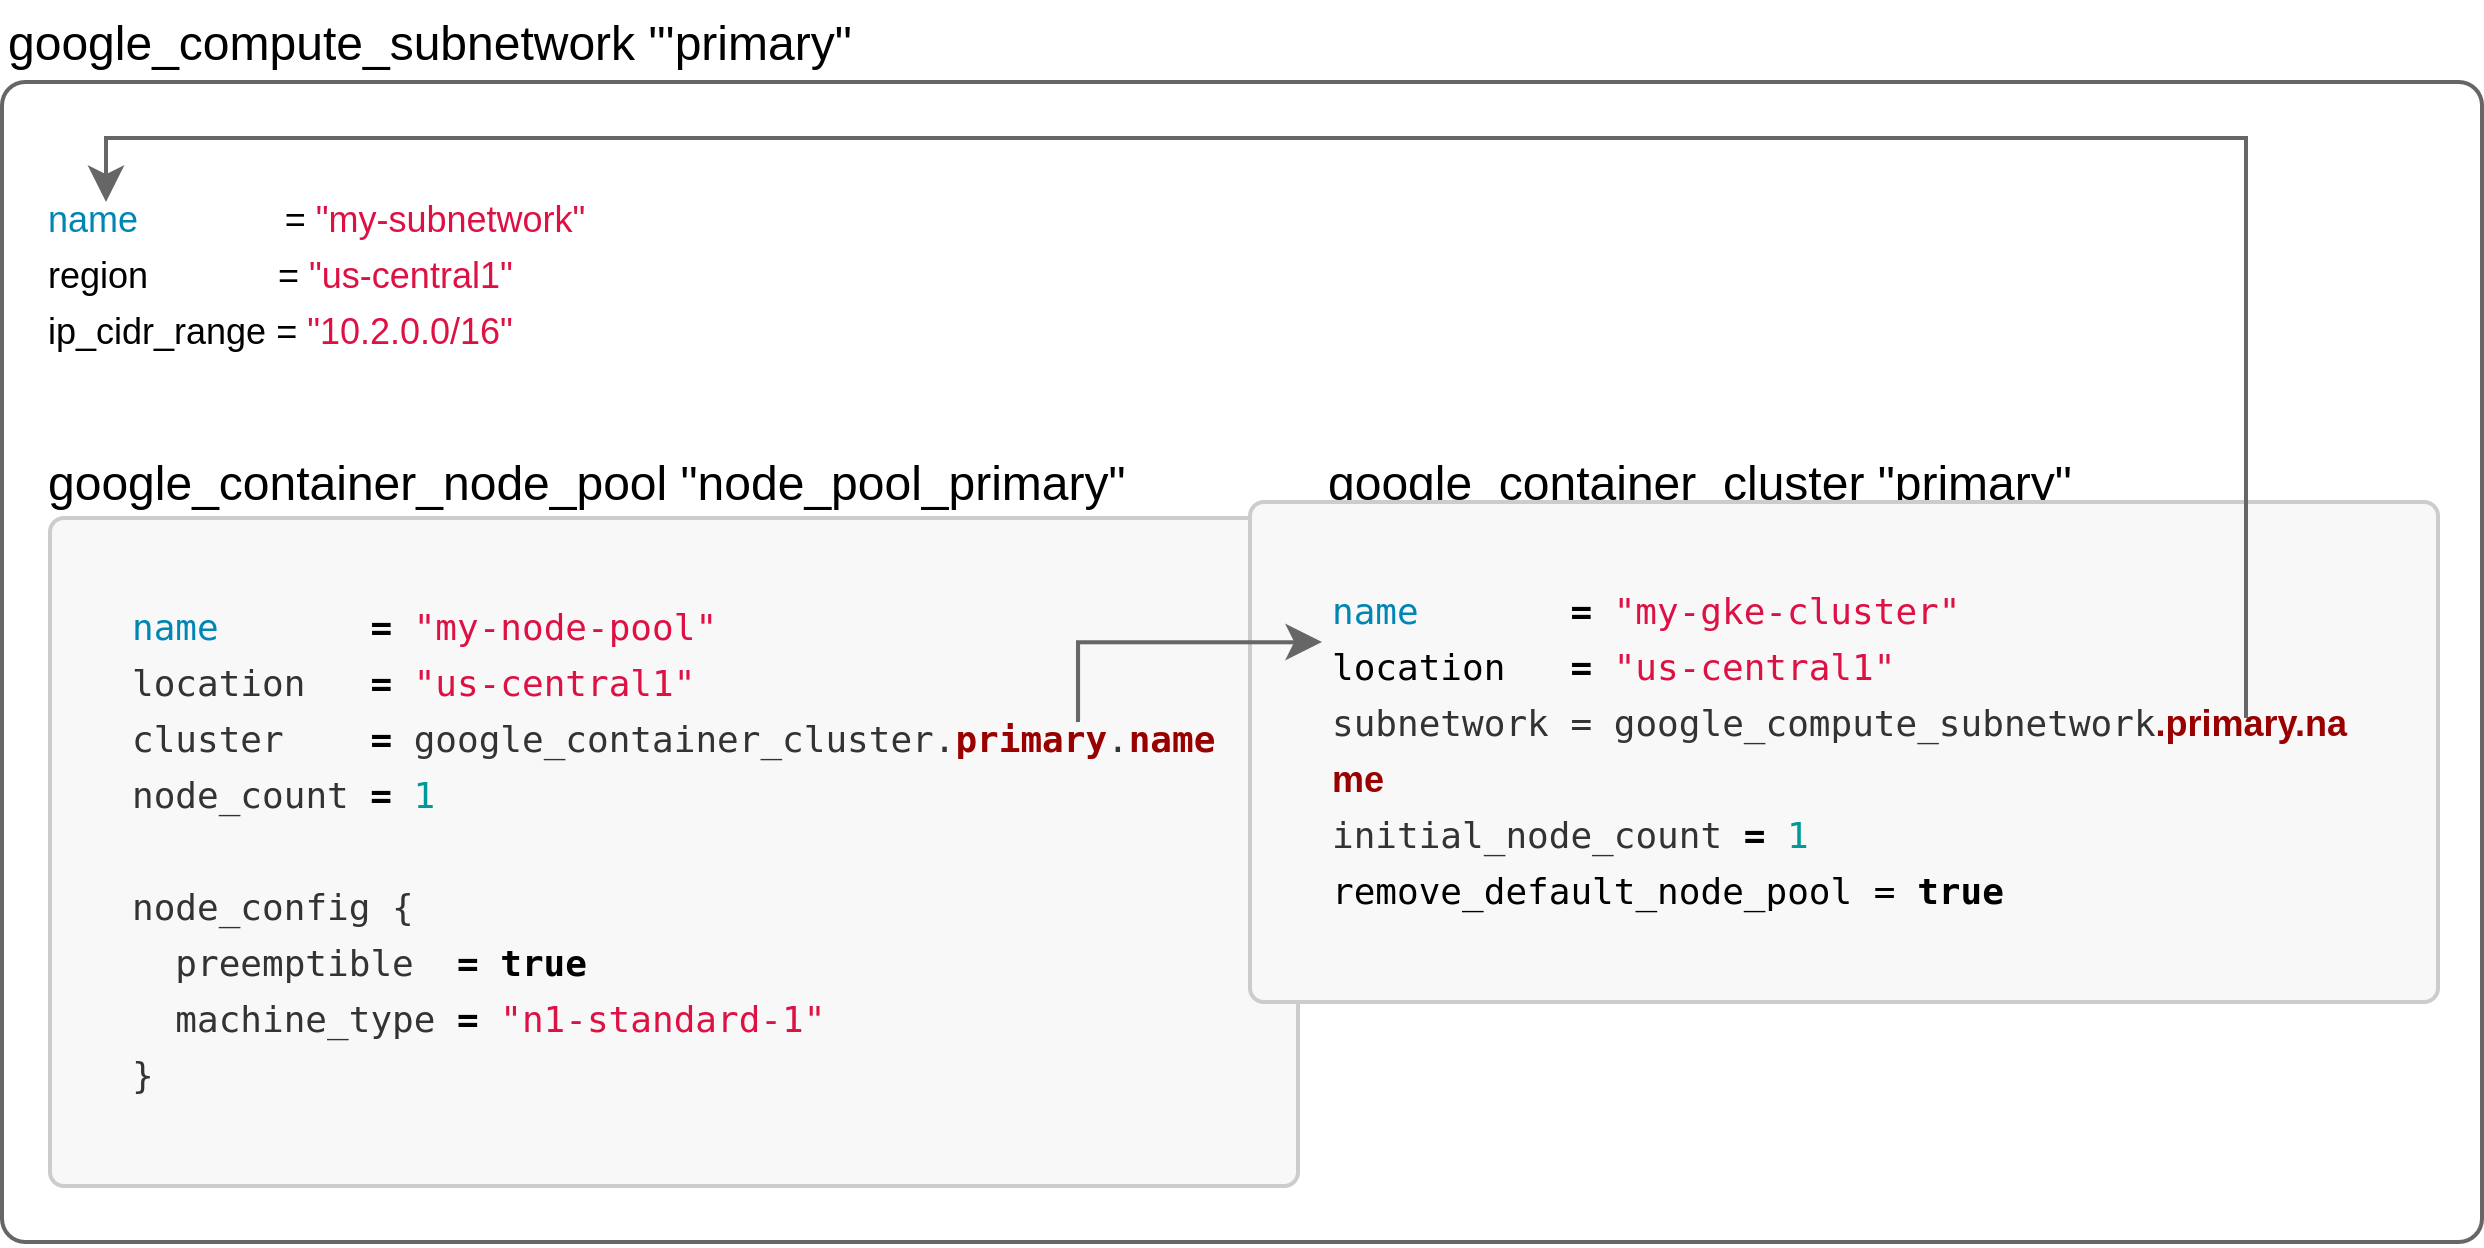
\includegraphics[width=0.9\textwidth]{terraform_gcp.png}
    \caption{k8s cluster provisioning with terraform in GCP}
    \label{fig:terraform_gcp}
\end{figure}

Since the order of execution of resource creation is computed by terraform, the following steps are performed. First a subnetwork is created within a given network and allocated a range of private IPs (this step, although unnecessary is preferred over using the default subnet for better isolation). Then the cluster object (control plane) is created and "nested" in the referred subnet. Finally, terraform creates the node pool without any nodes and declares it as a slave of the cluster object then spins up the amount of nodes and the appropriate resources that will be incorporated in the node pool. 

\pagebreak
\subsubsubsection{Customizing the base image with Packer}

\vspace{-5mm}\hspace{5mm} Due to SAP's corporate wide security checklist for production deployments, the default images\footnote{It is important to note the term image used in this section refers to that of the OS on which the virtual machines that constitute the k8s cluster and not docker images. 
As such, they have formats such as ISO, OVA and OVF.} on instances hosted by cloud providers (even Converged Cloud machines) are not security compliant. For reasons stated in Section (\ref{sec:reason}), setting up system requirements from the base image is not optimal for availability. 

On the other hand, one can create a base image with all the requirements and export it into a reusable base image. Enter \textbf{Packer}, an open source tool developed by Hashicorp which is uses that concept for creating identical machine images for multiple platforms from a single source configuration. Declarations consist of a set of \textbf{Builders} (responsible for creating machines and generating images from them for various platforms), \textbf{Provisioners} (to install and configure the machine image after booting) and \textbf{Post-Processors} (to upload, re-package artifacts). 

In our use case, the base image is the \textbf{Ubuntu Disco Dingo} (19.04) server install image. By leveraging Packer's boot command functionality, specific OS configurations are injected using \textbf{preseeding} (for instance apt setup, pre-partitioning, etc...). Then with the Ansible or Shell provisioner, the post-boot system requirements are installed. The image is then exported to the appropriate platforms defined if the build process succeeds.

Developping "PackerFiles" is a grueiling process due to the fact the VM build stage is not layered, any error would require an excruciatingly long complete rebuild. Therefore, using prebuilt templates such as Chef Bento\footnote{open source packer templates for building minimal Vagrant baseboxes for multiple platforms} is mandatory in order to maintain a decently fast workflow. 

\section{Designing a collaborative vulnerability knowledge base} \label{sec:vulnkb}

\hspace{5mm} The goal of the Community OSS CVE document store is to provide a community driven system of sharing information regarding vulnerable constructs and libraries for the vulnerability-assessment-tool. Different actors (pure consumers, security researchers, organizations) should be able to contribute and consume according to their own defined rules all without any central management actor. The subject of collaborative document store based on source version control tools such as git has been previously attempted in Phylesystem \cite{10.1093/bioinformatics/btv276} although requiring a centralized system that wraps interactions with the document store through an API. Our approach diverges in that it is distributed and consumption choices are delegated to the client.  

\subsection{Vulnerability statement declaration}

A statement regarding a vulnerability is, hereinafter defined as a declaration made at a certain point in time stating that a set of libraries possess a certain commit fix for a given vulnerability made by an actor. It is therefore restricted to an individual/organization at a given timestamp and multiple diverging or converging statements can be made by multiple actors at different times. The statements strictly follow the structure defined in Listing (\ref{list:statement}) and can contain two types of variables:
\begin{itemize}
    \item \textbf{exclusive}: if two statements have a different exclusive variable, it will be considered as conflicting.
    \item \textbf{cumulative}: if two statements have a different cumulative variable, it can be merged without major issues. For example if statement\_1 comming from individual\_1 adds a description of the CVE coming from a new source that statement\_2 from individual\_2 does not have, the aforementioned description can be added to statement\_2 without conflict.
\end{itemize}

The yaml file format is used because it grants balance between a strict, parseable structure and human readability (abstracts syntax and allows for adding descriptions unlike JSON). Along with the simplicity of the declaration, these design choices are destined to make contributions easy and possible by humans.

\subsection{Consuming the document store}

\begin{figure}[h]
    \centering
    \includegraphics[width=0.85\textwidth]{vulas_db_consumption.png}
    \caption{Consumption schema for the vulnerability knowledge base}
    \label{fig:vulas_db_consumption}
\end{figure}

Consuming the document store can be summarized by Figure (\ref{fig:vulas_db_consumption}). Multiple repositories (which in this case is a database) can contribute to the source consumption. Each of these repositories will be cloned locally and kept up to date with their remote periodically via git. Then, it is aggregated through a client-side content consumption software in order to be loaded into the vulnerability database. 

In order to allow users to define which vulnerability they would like to load into the database, a set of cumulative policies can be defined:

\begin{itemize}
    \item \textbf{Ordered list of trusted repositories}: assign a priority for each of the source repositories. If conflict were to occur, the merge operation will prioritize the one with higher priority.
    \item \textbf{Timestamp based}: prioritize latest bug statements
    \item \textbf{Maturity}: prioritize signed commits
    \item \textbf{Blacklist}: ignore statements regarding certain bugs
\end{itemize}

These policies are applied sequentially, if policy\_1 is not able to merge an array of statements, its \textbf{arbiter} (policy\_2) is called upon. This chain of policies ensures that all edge case of the merge operation is covered whilst granting the user the appropriate granularity for defining his consumption preference. Implementation wise, the consumption rules by a yaml whose structure is defined in Listing (\ref{list:consumption}).

In order to keep accountability of the merged statements, a \textbf{final statement} (with the structure defined in Listing (\ref{list:final})) is created and stored locally after all merge operations are applied. The granularity of these "transaction logs" are per attribute, any changes occurring to an attribute in any statement are cached. 

\subsection{Contributing to the knowledge base}

This proposition is meant to address distributed methods of allowing contribution to the vulnerability knowledge base from an environment with untrusted actors. In our approach, each contributor maintain their own distinct repository in which they issue statements regarding a CVE affecting certain libraries (their identities being guaranteed by their identity on Github). As a further mean of ensuring the source of a commit, contributors can add their public GPG keys to the repository and sign every commit with the private key in the keypair. 

Every statement is nested under the \textit{data} directory and their separate folder defined by their cve id (lower cased). In each repo, a statement can be declared using a file named \textit{statement.yaml}. The repository can also be signed by publishing the public signature in the \textit{signature} directory, in which case, every commit regarding a particular statement must also be signed.

Once this repository structure is respected, the actors can chose two modes of contribution (see Figure (\ref{fig:vulas_db_contribution}) for a summary):

\begin{itemize}
    \item \textbf{Manual}: manually add a statement to the version control and sign if required
    \item \textbf{Automatic}: using a content export software, periodically update the repository from an export (see Listing (\ref{list:contrib}) for the configuration structure chosen) of the current running database. The vulnerabilities can then be filtered using a series of user defined policy to exclude certain bugs (for instance internal ones).
\end{itemize}

\vspace{2mm}
\begin{figure}[h]
    \centering
    \includegraphics[width=0.7\textwidth]{vulas_db_contribution.png}
    \caption{Contribution schema for the vulnerability knowledge base}
    \label{fig:vulas_db_contribution}
\end{figure}

\subsection{Implementation}

Golang was chosen as the implementation language for the content import and export software due to the fact that it is typed (useful for implementing strict enforcement of statements), compiled (lighter footprint, easier distribution as a CLI\footnote{Command Line Interface}) and a decent trade-off between performance and development time. Libraries such as Cobra\footnote{Commander for modern Go CLI interactions, source: https://github.com/spf13/cobra} were used to build a functional CLI and Viper\footnote{Configuration solution for Go applications, source: https://github.com/spf13/viper} to program a functional configuration parser. However, due to Go's lack of generics and class concepts (inheritance through structure embedding), the main downside of using this language is that the code base includes a lot of repetitive code.

Because of the lack of time, the implementation of this document store is still Work In Progress (required functionalities are implemented but code coverage is quite low and further refactoring is necessary). 


\pagebreak
\section{Cloud provider benchmark}

\hspace{5mm} Due to corporate decisions to move all infrastructures maintained by the Security Testing team to public cloud providers (as opposed to SAP's Converged Cloud), this benchmark is done in order to help in the process of deciding which public provider to migrate to. Three public cloud offers are studied (GCP (Google Cloud Platform), AWS (Amazon Web Service) and Microsoft Azure) in comparison to the private solution. 

\subsection{Computing offer comparison}

\hspace{5mm} It is important to note that all the aforementioned providers have support for Linux as well as Windows VMs. Although terminologies vary widely between providers (machine type for GCP, instance for AWS, VM for Azure), they all provide a couple of essential categories of common machine families. This benchmark of computing offers will focus mainly on the spread and diversity of computing instance offers through the lens of the computing ratio variable (amount of vCPU per GiB of memory). Using different methods of dynamically fetching the different computing instance offers from the cloud providers, we examined the following family types:

\begin{itemize}
    \item \textbf{General purpose} instances provide a balance of compute, memory and networking resources, and can be used for a variety of diverse workloads. These instances are ideal for applications that use these resources in equal proportions such as web servers and code repositories and are offered by all of the aforementioned providers.
    \item \textbf{Memory optimized} are ideal for tasks that require intensive use of memory with higher memory-to-vCPU ratios than the N1 high-memory machine types. These machine types are suited for in-memory databases and in-memory analytics, such as SAP HANA and business warehousing (BW) workloads, genomics analysis, SQL analysis services, ....
    \item \textbf{Compute-optimized} machine types are ideal for compute-intensive workloads.
\end{itemize}

The instance performance (vCPUs, memory(GiB)) and family type are then computed in order to generate boxplots with the preferred grouping (by cloud provider, by family, etc...). 

\begin{figure}[h]
    \centering
    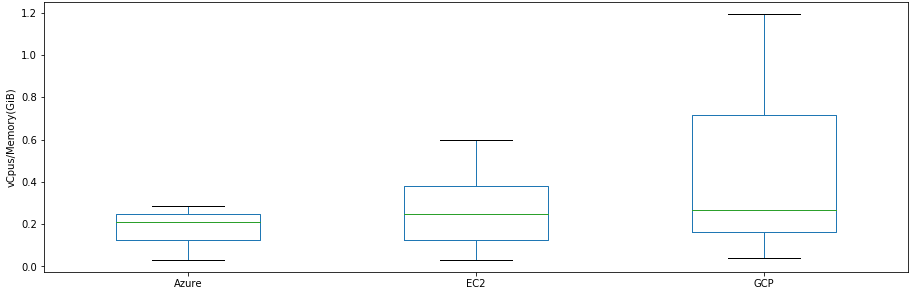
\includegraphics[width=\textwidth]{bench_computing_provider.png}
    \caption{Boxplot of compute ratio per cloud provider}
    \label{fig:bench-ratio-provider}
\end{figure}

A comparison of the computation/memory ratios (see Figure (\ref{fig:bench-ratio-provider})) between providers shows that GCP has the most diverse offers when it comes to vCpus/Memory despite having a lower amount of machine types than other providers. It is also noticeable (within the given dataset) that GCP and AWS EC2 tend to offer a higher Computation/Memory ratio than Azure whose spread is the lowest.

\begin{figure}[h]
\subfloat[Grouped by provider class]{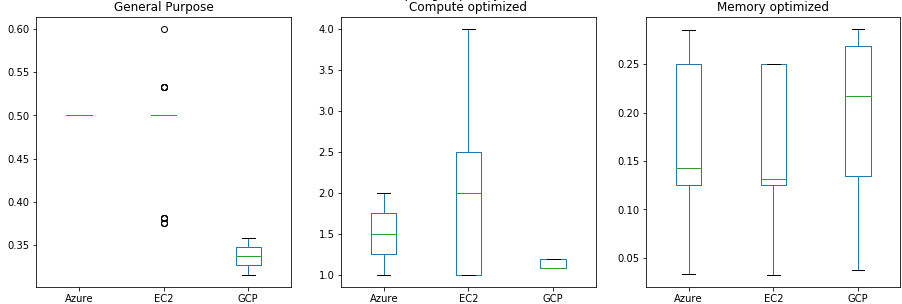
\includegraphics[width=0.95\textwidth]{bench_computing_provider_ratio.png}\label{fig:bench_ratio_provider}}

\subfloat[Grouped by ratio class]{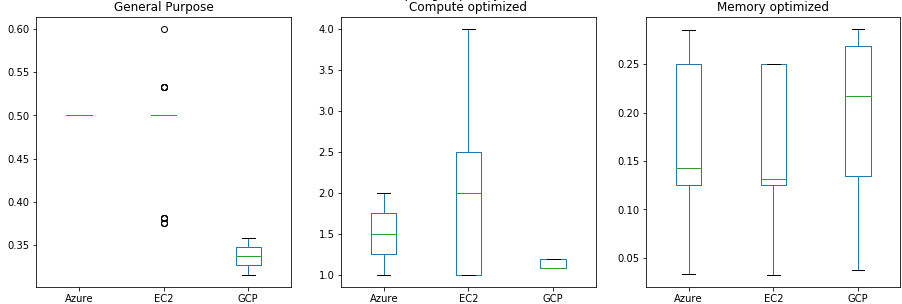
\includegraphics[width=0.95\textwidth]{bench_computing_provider_ratio.png}\label{fig:bench_ratio_class}}
\caption{Box plot of computing ratios grouped per criteria}
\end{figure}

Outliers excluded, GCP General Purpose seems to offer the most variety (see Figure (\ref{fig:bench_ratio_provider})), however their Compute optimized and Memory optimized offers are quite lacking compared to their counterparts. This is more telling of a different nomenclature between the cloud providers and does not grant us much insight into the diversity of their offers.

By applying the classification labels to the actual ratio, we get a more complete picture (see Figure (\ref{fig:bench_ratio_class})). AWS excels in compute optimized instance in comparison to other providers whereas GCP and Azure take the lead in memory optimized instances. On the other hand, with general purpose machines, AWS maintains a higher spread ratio whilst GCP mainly focuses on the lower proportion of the spectrum.

\subsection{Hosted database offers}

\hspace{5mm} In this section, the different cloud providers will be used as the backbone for comparing the advantages and drawbacks of using a hosted database rather than running a self administered database cluster in k8s. Specifically a version of the vulnerability-assessment-tool database will be loaded onto a hosted database instance (with or without replication) and a self administered k8s cluster to compare their price, migration cost as well as their operational cost.

\subsubsection{Cost}

\hspace{5mm} In order to establish a proper price comparison, a set of different cases for resource consumptions are defined: 
\begin{itemize}
    \item \textbf{Lightweight HA} : the cluster is instantiated with no prior scan and data, then, the bugs are loaded using the patch-analyzer. This deployment is not destined for high availability or resilience (therefore with less replicas, no auto-scaling) and is optimal for small testing environments with a 6 month usage buffer with the sufficient amount of replicas that will ensure high availability and resilience.
    \item \textbf{Medium Load HA} : the cluster is instantiated with no prior scan and data, then, the bugs are loaded using the patch-analyzer. This deployment is not destined for high availability or resilience (therefore with less replicas, no auto-scaling) and is optimal for small production environments with a 2 year buffer with the sufficient amount of replicas that will ensure high availability and resilience.
    \item \textbf{Production Load HA} : the cluster is loaded with the latest dump of the internal SAP vulnerability-assessment-tool database (which at the time of this document creation is around 350GB). This deployment is not destined for high availability or resilience and is optimal for production environments with a 3-5 year usage buffer. This data load includes app specific data (once those are removed, the database size is around 150GB in our current setup) with the sufficient amount of replicas that will ensure high availability and resilience.
    \item \textbf{Hosted DB} : for using a pre-existing database (for cloud providers such as GCP, AWS, Azure, etc...) which require lower resources as the database are no longer self managed.
\end{itemize}

\vspace{3mm}
From each of these deployment case, a range of resource list is calculated; from the minimum to the maximum amount of CPU and Memory (GiB), the amount of Persistent Volumes (GiB) and the cost of the hosted database instance if required. Then using GCP cost calculator, the cost for each case is computed. Note that this methodology overestimates by a big margin the cost of computing resources (CPU, Memory) because it assumes that all machines will consume $100\%$ of the allocated resource continuously (24/7) for one month. Mapping the appropriate deployment cases to its PVC size, the relative difference in cost between a hosted and non hosted HA deployment can be measured using the estimated cost range. 

\pagebreak
The price comparison is applied in two regions, eu-west-2 (one of the most expensive regions in GCE) and us-central-1 (one of the cheapest regions in GCE), to establish a possible evolution range of the difference in cost. In both cases, the hosted deployment becomes profitable over the self managed cluster when the data load surpasses 200GB (see Figure (\ref{fig:bench_vulas_price})). 

\begin{figure}[h]
    \subfloat[eu-west-2]{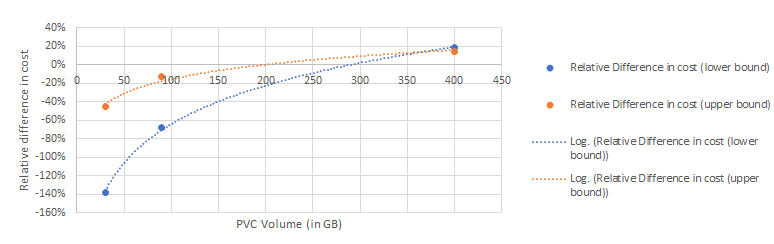
\includegraphics[width=\textwidth]{bench_vulas_price_eu_west2.png}\label{fig:bench_vulas_price_eu_west_2}}
    
    \subfloat[us-central-1]{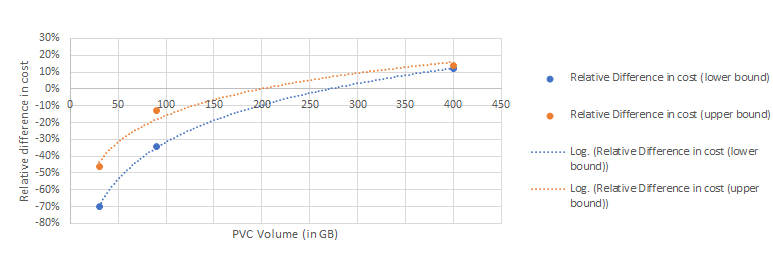
\includegraphics[width=\textwidth]{bench_vulas_price_us_central1.png}\label{fig:bench_vulas_price_us_central_1}}
    \caption{Relative difference in cost between a self managed and hosted PostgreSQL}
    \label{fig:bench_vulas_price}
\end{figure}

\subsubsection{Services}

\hspace{5mm} Unlike self managed database clusters, snapshots, backups and maintenance windows are options which can be added for most hosted database offer by cloud providers without extra operational cost (testing, developing and maintaining these scripts). However the most interesting feature is database storage auto resizing which ensures its vertical scalability. The hosted database service main drawback is that root access is not allowed, so in order to migrate from an external database, the dump has to be done without owner or privileges. This minor setback is however minuscule compared to the advantages cited previously.

\subsubsection{Performance}

\hspace{5mm} The performance benchmark is run on each cloud provider (each with comparable amount of resources) with the full vulnerability-assessment-tool production workload (350GB of data, without trimmed application and space related data) against a script of read-only requests (same script and pgbench parameters as described in Section (\ref{sec:connection_pool_bench})).

\textbf{Test cases}:
\begin{itemize}
    \item \textbf{GCP (helm)}: using the self managed HA postgres with replication and pooling
    \item \textbf{GCP (cloudSQL non optimised)}: using the CloudSQL Postgres offer with no production configuration and only a single instance without read replicas
    \item \textbf{GCP (cloudSQL optimised)}: using the CloudSQL Postgres offer with production configuration (see Listing (\ref{list:prod})) and only a single instance without read replicas
    \item \textbf{GCP (cloudSQL optimised)}: using the CloudSQL Postgres offer with production configuration and only a single instance without read replicas and 400GB of SSD (increases IOPs drastically over the bare minimum at 257GB)
    \item \textbf{GCP (cloudSQL optimised, 1 replica)}: using the CloudSQL Postgres offer with production configuration and only a single instance with read replicas and pg\_bench querying a pgpool statefulset with 3 replicas.
    \item \textbf{AWS (helm)}: using the self managed HA postgres with replication and pooling
    \item \textbf{AWS (rds non optimised)}: using the RDS PostgreSQL offer without implementing production configuration and only a single instance witout read replicas
    \item \textbf{AWS (rds optimised)}: using the RDS PostgreSQL offer with production configuration and only a single instance without read replicas
    \item \textbf{AWS (rds optimised, 1 replica)}: using the RDS Postgres offer with production configuration and only a single instance with read replicas and pg\_bench querying a pgpool statefulset with 3 replicas.
    \item \textbf{Azure (helm)}: using the self managed HA postgres with replication and pooling
    \item \textbf{Azure (hosted non optimized)} : using the RDS PostgreSQL offer without implementing production configuration and only a single instance witout read replicas. However, due to the lack of possible configurations (most configuration listed below being unavailable or unchangeable), the optimized version will not be represented.
\end{itemize}

Note that as the performance of the Azure deployment is too poor (being the outlier in every case and making the charts non exploitable), the charts shown below do not include Azure. Due to the fact that the helm chart has been developed and optimized for Converged Cloud, its performance will likely be better than other test cases. In order to not overclutter the charts, the following colour coding convention is used: \textcolor{AWS}{AWS}, \textcolor{Azure}{Azure}, \textcolor{GCP}{GCP}. 

% Please add the following required packages to your document preamble:
% \usepackage[table,xcdraw]{xcolor}
% If you use beamer only pass "xcolor=table" option, i.e. \documentclass[xcolor=table]{beamer}
\begin{table}[!ht]
    \centering
    \begin{tabular}{|c|l|c|l|l|l|l|}
    \hline
    \textbf{provider} & \multicolumn{1}{c|}{\textbf{helm}} & \textbf{hosted}       & \multicolumn{1}{c|}{\textbf{optimised}} & \multicolumn{1}{c|}{\textbf{replicated}} & \multicolumn{1}{c|}{\textbf{bigssd}} & \multicolumn{1}{c|}{\textbf{mean latency}} \\ \hline
    azure             & \multicolumn{1}{c|}{x}             & \multicolumn{1}{l|}{} &                                         &                                          &                                      & 1.9E+04                                    \\ \hline
    gcp               & \multicolumn{1}{c|}{x}             & \multicolumn{1}{l|}{} &                                         &                                          &                                      & 1.3E+04                                    \\ \hline
    aws               & \multicolumn{1}{c|}{x}             & \multicolumn{1}{l|}{} &                                         &                                          &                                      & 1.2E+04                                    \\ \hline
    ccloud            & \multicolumn{1}{c|}{x}             & \multicolumn{1}{l|}{} &                                         &                                          &                                      & 8.1E+03                                    \\ \hline
    gcp               &                                    & x                     & \multicolumn{1}{c|}{x}                  & \multicolumn{1}{c|}{x}                   & \multicolumn{1}{c|}{x}               & 1.0E+04                                    \\ \hline
    aws               &                                    & x                     & \multicolumn{1}{c|}{x}                  & \multicolumn{1}{c|}{x}                   & \multicolumn{1}{c|}{x}               & 1.2E+04                                    \\ \hline
    gcp               &                                    & x                     & \multicolumn{1}{c|}{x}                  & \multicolumn{1}{c|}{x}                   &                                      & 1.0E+04                                    \\ \hline
    azure             &                                    & x                     & \multicolumn{1}{c|}{x}                  & \multicolumn{1}{c|}{x}                   &                                      & 6.9E+04                                    \\ \hline
    gcp               &                                    & x                     & \multicolumn{1}{c|}{x}                  &                                          &                                      & 1.0E+04                                    \\ \hline
    aws               &                                    & x                     & \multicolumn{1}{c|}{x}                  &                                          &                                      & 1.2E+04                                    \\ \hline
    gcp               &                                    & x                     &                                         &                                          &                                      & 4.2E+04                                    \\ \hline
    aws               &                                    & x                     &                                         &                                          &                                      & 4.6E+04                                    \\ \hline
    azure             &                                    & x                     &                                         &                                          &                                      & 7.1E+04                                    \\ \hline
    \end{tabular}
    \caption{Average latency (ms) per deployment setup}
    \label{tab:bench_vulas_latency}
    \vspace{-3mm}
\end{table}

It is demonstrable that using the cloud provider database as a service offer using naive configuration (without tailoring it to the production workload) is detrimental, as for AWS, GCP as well as Azure the query latency is almost 4 times the naive helm chart deployment.


On the other hand, with replication and tailored production configuration, the hosted database offer certain performance gain as well as price benefits (lower overhead cost as well as base cost). On the other hand, since performance can be gained using bigger SSDs (increased IOPs), one can use this to optimize the database, but an increase of 100GB in the ssd size won't offer much of a gain in latency (as seen by the similar outcomes for big-ssd deployments). 

\begin{table}[h]
\centering
\begin{tabular}{|c|c|c|c|c|c|}
\hline
\textbf{count} & \textbf{mean} & \textbf{std} & \textbf{min} & \textbf{50\%} & \textbf{max} \\ \hline
10             & 0.002609      & 0.000599     & 0.000152     & 0.002742      & 0.003633     \\ \hline
\end{tabular}
\caption{Relative difference statistics between deployment and reference}
\label{tab:diff}
\end{table}

These query latencies are not affected by the network latency, nor by the speed of the connection establishing due to the fact that the relative difference between tps (transaction per second) with and without handshake is relatively low: with a mean of $0.0026\%$ and a standard deviation of $0.0005$ points (see Table \ref{tab:diff})).

Grouping by complexity (arbitrary decision on the mean of all latency results for all providers), confirms the fact that GCP optimised seems to be the one whose performance in most case closest and some cases better than the CCloud native helm chart. The sample of query given do not however represent the frequency of their usage, therefore, a weighted approach (with usage $frequency \times cost$) would give a better approximation of the actual performance of the vulas database in each scenario. It would also be interesting to group the queries into their operation type (for instance seq\_scan, index\_scan, nested\_loop, etc.) in order to gauge the performance of the database for each operation per cloud provider.

\subsection{Performance benchmark}

\hspace{5mm} In order to evaluate in an unbiased manner the performance of each cloud provider, we'll base ourselves on the PerfKitBenchmarker\footnote{set of benchmarks to measure and compare cloud offerings developed and open-sourced by GoogleCloudPlatform, source: https://github.com/GoogleCloudPlatform/PerfKitBenchmarker} for Database, Networking and Instance performance and perf-test\footnote{performance test kit for kubernetes deployments, source: https://github.com/kubernetes/perf-tests} for provided control plane performance.

\textbf{Reproduction environment}:

\begin{table}[h]
\centering
\begin{tabular}{|l|l|l|l|l|}
\hline
\textbf{Cloud name} & \textbf{Default Zone} & \textbf{Machine Type} & \multicolumn{1}{c|}{\textbf{vCPUs}} & \multicolumn{1}{c|}{\textbf{Memory (GiB)}} \\ \hline
GCP                 & us-central1-a         & n1-standard-1         & 1                                   & $\sim$3.5                                  \\ \hline
AWS                 & us-east-1a            & m3.medium             & 1                                   & 3.75                                       \\ \hline
Azure               & eastus2               & Standard\_A1          & 1                                   & 2.1                                        \\ \hline
\end{tabular}
\caption{Default reproduction environment for PerfKitBenchmarker}
\end{table}

Note that the previous machine types may vary slightly depending on the test applied (due to different resource requirements). The default machine type is meant to be as close together as possible, however Azure's machine type is a bit less performant than the others, which might disadvantage it. AWS should however profit from this disparity during the benchmarks.

On the other hand, all regions tested are within the US, so comparable results should be observed and the regional factor should not influence the results.

\subsubsection{Computing instance}
\hspace{5mm} The cloud provider instance performance can be evaluated thanks to aggregating data from the unixbench benchmark group which cover tests ranging from computing, pipe performance, system calls, to unix file copies.

\subsubsubsection{Basic arithmetics}

\vspace{-5mm} Drystone is a synthetic benchmark application meant to mimic a real life application with a mix of mathematical and other operations (with the following specifications: Integer performance predominated, with little or no floating-point calculations, and could be contained inside small memory subsystems). This benchmark, although lightweight and quite portable, is susceptible to compiler optimization interference (as it is written in C) and only captures a tiny fraction of mathematical and basic operations. Because these inherent flaws are also present in the Wheststone test, data from these benchmarks are excluded.

\subsubsubsection{Pipe throughput}

\vspace{-5mm} This test (composed of two tests Pipe throughput and Pipe-based Context Switching) intends to evaluate pipe performances (A pipe being the simplest form of communication between processes) by measuring the amount of lines executed per seconds (lps).

\begin{figure}[!h]
    \captionsetup[subfigure]{labelformat=empty}
    \centering
    \subfloat[]{\includesvg[width=0.7\textwidth]{bench_pipe_throughput.svg}}

    \vspace{-5mm}
    %\includesvg[width=0.8\textwidth]{bench_pipe_throughput_stats.svg}
    \subfloat[]{
        \begin{tabular}{|c|c|c|c|}
        \hline
        \textbf{provider} & \textbf{\begin{tabular}[c]{@{}c@{}}pipe throughput\\ (lps)\end{tabular}} & \textbf{\begin{tabular}[c]{@{}c@{}}pipe based context \\ switching (lps)\end{tabular}} & \textbf{\begin{tabular}[c]{@{}c@{}}relative performance \\ ratio (\%)\end{tabular}} \\ \hline
        aws               & 409657                                                                   & 73558.4                                                                                & 17.96                                                                               \\ \hline
        azure             & 366060.6                                                                 & 95920.7                                                                                & 26.20                                                                               \\ \hline
        gcp               & 1097697                                                                  & 137761.1                                                                               & 12.55                                                                               \\ \hline
        \end{tabular}
    }   
    \vspace{-3mm}
    \caption{Pipe performance (lps) per cloud provider}
    \label{fig:bench_pipe}
\end{figure}

Pipe throughput is the number of times (per second) a process can write 512 bytes to a pipe and read them back. The pipe throughput test has no real counterpart in real-world programming. The context switching measures the number of times two processes can exchange an increasing integer through a pipe. 

The pipe-based context switching test is more like a real-world application. The test program spawns a child process with which it carries on a bi-directional pipe conversation. The relative difference between pipe throughput and pipe based context switching (due to added the added complexity) is minimized in GCP's case.

\subsubsubsection{Shell and process calls}

\vspace{-5mm} The process creation test measures the number of times a process can fork and reap a child that immediately exits. Process creation refers to actually creating process control blocks and memory allocations for new processes, so this applies directly to memory bandwidth. Typically, this benchmark would be used to compare various implementations of operating system process creation calls. The shells scripts test measures the number of times per minute a process can start and reap a set of one and eight concurrent copies of shell script where the shell script applies a series of transformation to a data file. Due to shell scripts extra complexity, it is expected that the performance would be lower that the pure process creation. 

\begin{figure}[!h]
    \centering
    \captionsetup[subfigure]{labelformat=empty}
    \subfloat[]{\includesvg[width=0.8\textwidth]{bench_shell.svg}}
    
    \vspace{-5mm}
    % \includesvg[width=0.8\textwidth]{bench_shell_stats.svg}
    \subfloat[]{
        \begin{tabular}{c|c|c|c|}
        \cline{2-4}
        \textbf{}                                                                                                             & \textbf{aws} & \textbf{azure} & \textbf{gcp} \\ \hline
        \multicolumn{1}{|c|}{\textbf{\begin{tabular}[c]{@{}c@{}}process \\ creation (lps)\end{tabular}}}                      & 4880.4       & 4647.4         & 11070        \\ \hline
        \multicolumn{1}{|c|}{\textbf{\begin{tabular}[c]{@{}c@{}}1 concurent \\ shell (lps)\end{tabular}}}                     & 3339.7       & 3440.4         & 7771.7       \\ \hline
        \multicolumn{1}{|c|}{\textbf{\begin{tabular}[c]{@{}c@{}}8 concurrent \\ shell (lps)\end{tabular}}}                    & 435          & 426.4          & 999.2        \\ \hline
        \multicolumn{1}{|c|}{\textbf{\begin{tabular}[c]{@{}c@{}}performance lost \\ from shell overhead (\%)\end{tabular}}}   & -86.97       & -87.60         & -87.14       \\ \hline
        \multicolumn{1}{|c|}{\textbf{\begin{tabular}[c]{@{}c@{}}performance lost \\ from concurrent shell (\%)\end{tabular}}} & -31.57       & -25.97         & -29.79       \\ \hline
        \end{tabular}
    }
    \vspace{-3mm}
    \caption{Process creation performance (lps) per cloud provider}
    \label{fig:bench_pipe}
\end{figure}

Concurrent shell execution seems to be a road block on all providers as the execution speed in lpm (lines per minute) drop significantly (at the same ratio as the amount of concurrent executions). This however comes from the Linux kernel implementation as well as mutex locks on the data file and not from the cloud providers themselves. The performance drop due to concurrent execution is quite similar all throughout providers; the 8 concurrent shell execution having around $12\%$ to $13\%$ of process number finished of the single shell execution. The same observation can be made for the shell overhead. Despite the similar relative drops, the base process call performance of GCP remains the highest which, in turn, translates to their instances being the most optimized for shell and process calls.

\subsubsubsection{Conclusion}

\vspace{-5mm}\hspace{5mm} Instance performances measured through the unix-bench kit show that GCP instances are the most optimized with AWS and Azure following closely behind. This difference possibly comes from different implementation of the base image; GCP using a \textit{Container Optimized OS} based on Chromium OS, AWS using \textit{Amazon Linux AMI} and Azure using the \textit{Canonical Ubuntu}. However, this is mere speculations because the design documents for these images do not go into detail about their implementation.

\subsubsection{Databases and filesystem}

\subsubsubsection{Fio — I/O speed}

\vspace{-5mm}\hspace{5mm} Fio is short for Flexible IO, a versatile IO workload generator. In this benchmark, each provider provision one equivalent machine type and performs a series of sequential or random operations such as reads or writes of a $10 \times 10 \times 1000$ mb file with a given block size in bytes (kilobytes) and a given iodepth (Number of IO operations is issues to the OS at a given time). This would give an idea of IOPs for each provider and the underlying performance of their file system. In detail, the disk access pattern benchmarked are the following:

\begin{itemize}
    \item \textbf{Random read}: blocks of 4kb are read from random locations on the surface of the device at an IOdepth of 1. This access pattern is quite common during operating system startup, where lots of configuration and driver files must be read from the disk and can therefore give an insight into instance startup or reboot. 
    \item \textbf{Random write}: blocks of 512kb are written from random locations on the surface of the device at an IOdepth of 1. This type of access pattern is common when running applications from a disk and also when copying large application directories.
    \item \textbf{Sequential read}: contiguous blocks of 4kb are read/write from adjacent locations on the surface of the device at an IOdepth of 1. This type of access pattern is common when reading large files. 
    \item \textbf{Sequential write}: contiguous blocks of 512kb are read/write from adjacent locations on the surface of the device at an IOdepth of 1. This type of access pattern is common when writing large files.
    \item \textbf{Random Parallel read}: the fio process will try to submit 64 simultaneous I/O, each attempting to random write a 4kb blocksize. 
\end{itemize}

With the above job config, fio gathers two metrics \textbf{IOps} and \textbf{Latency per operation}. The latter is used because it is richer, giving access to each percentile of the latency distribution. This data is aggregated in Figure (\ref{fig:bench_fio}) which allows us to study in depth each provider's io operation latency and Table (\ref{tab:bench_fio}) for specific data of the median and the 95\textsuperscript{th} percentile.

\begin{figure}[!h]
    \centering
    \subfloat[Random read]{\includesvg[width=0.5\textwidth]{bench_fio_random_read.svg}}\subfloat[Sequential read]{\includesvg[width=0.5\textwidth]{bench_fio_sequential_read.svg}} 
    \newline
    \subfloat[Random write]{\includesvg[width=0.5\textwidth]{bench_fio_random_write.svg}}\subfloat[Sequential write]{\includesvg[width=0.5\textwidth]{bench_fio_sequential_write.svg}}
    \newline
    \subfloat[Random parallel read ]{\includesvg[width=\textwidth]{bench_fio_random_parallel_read.svg}}

    \caption{Latency percentile (log ms) distribution for IO operations}
    \label{fig:bench_fio}
\end{figure}

From this point onwards, two criterias are measured; \textbf{Performance} (characterized by the median latency ($p50$)) and \textbf{Stability} (characterized by the standard deviation of the sample).

\textbf{Write operations}

For random writes, all instances offer stable performance with a homogeneous percentile distribution (the difference between the 1\textsuperscript{st} and 90\textsuperscript{th} percentile is relatively close). GCP excels in this category with a the lowest median (502 $\mu$s) and p95 (1608 $\mu$s).

For sequential writes, Azure takes the lead with a median at 31104$\mu$s. However, both AWS and Azure suffer from stability (with standard deviations over 7 times bigger that GCPs) whereas GCP's is more stable with the highest median of around 444416$\mu$s. 

\vspace{3mm}
\textbf{Read operations}

When it comes to sequential reads, Azure takes the lead on performance but GCP overtakes it on stability. As for random reads, AWS is the favoured in both those categories. Finally, for random parallel reads, AWS beats both other providers for performance (median at 18560 $\mu$s) with gcp acing stability (with the lowest standard deviation).

\textbf{Conclusion}

It is important to note that random access seems to be outperforming sequential ones in both operation types, which is impossible whether it is in the case of an HDD\footnote{Hard disk drive} (time to seek to random segments of the disk should add up to a higher latency) or of an SSD\footnote{Solid state drive} (the overhead cost of initiating IO operations should make random access less performant). This observation can possibly be explained in part due to the fact that the total size of the file written to disk exceeds the default SSD size attached to the machine which would then require scaling up or adding a PV, causing the higher latency.

If the following hypothesis were true, we can confirm the observation that none of the provider file system performance outperforms each other in all disk access pattern. And that for overall file system performance, one should choose AWS and for stability GCP. 

\subsubsubsection{Redis — key value data stores}

\vspace{-5mm}\hspace{5mm} The redis benchmark is based on creating equivalent computing instances (VMs in Azure, EC2 instance in AWS and Machines in GCP) running a single node redis database and querying it (with update, read and insert operations) from multiple computing instances each running a specific amount of threads (the amount of threads being the varying parameter between metric measurement). As redis is an open source (BSD licensed), in-memory data structure store, used as a database, cache and message broker, this benchmark would also give an idea as to the efficiency of in memory storage in each of the respective provider computing instances.

We mainly base our comparison of redis performance on throughput and latency. As those two are closedly tied together, the data collected mainly focuses on the former which is the number of operations processed by the database within a given period of time. Graphing the throughput evolution per concurrent server (redis) threads and fitting it to a function would give an idea of the performance for redis that can be gained from vertical scaling. Fitting the distribution with a logarithmic function works perfectly with AWS and Azure with a low coefficient of determination ($R^2 \geq 0.97$) but not well with GCP.

\begin{figure}[h]
    \centering
    \begin{adjustwidth}{-.5in}{-.5in}  
    \begin{minipage}{.6\textwidth}
        \includesvg[width=\textwidth]{bench_redis_throughput.svg}
    \end{minipage}
    \begin{minipage}{.3\textwidth}
        $\begin{aligned}
        \textbf{\textcolor{AWS}{aws}} &:
            \begin{cases}
                x &= 7312 \times ln(x) + 1433 \\
                R^2 &= 0.971
            \end{cases} \\
        \textbf{\textcolor{Azure}{azure}} &:
            \begin{cases}
                x &= 6476 \times ln(x) - 2038 \\
                R^2 &= 0.981
            \end{cases} \\
        \textbf{\textcolor{GCP}{gcp}} &:
            \begin{cases}
                x &= 17195 \times ln(x) + 33993 \\
                R^2 &= 0.729
            \end{cases} \\
    \end{aligned}$
    \end{minipage}
    \end{adjustwidth}
    \caption{Redis throughput (req/s) per number of server threads}
    \label{fig:bench_redis}
\end{figure}

Each provider reaches an optimal throughput after a certain point and the growth is then stunted. This plateau occurs at $100 000$ requests/sec for GCP, $40 000$ requests/sec for AWS and $35 000$ requests/sec for Azure. GCP is therefore the most fitted for redis database hosting.

\subsubsubsection{MongoDB — document oriented databases}

\vspace{-5mm}\hspace{5mm} MongoDB is a general purpose, document-based, distributed database. The mongo YCSB benchmark\footnote{Yahoo! Cloud Serving Benchmark, source: https://github.com/brianfrankcooper/YCSB} is meant to provide a well rounded picture of a system’s performance using in our case a database with 1000000 records, with an equivalent client machine performing 10000 operations with 32 clients with a varying proportion of read, insert and update and 1 server machine serving with 32 threads. 

Using the percentile distribution of the latency (in ms, scaled down to logarithmic scale) for certain CRUD operations (read, insert, update without bulk or delete operations) in Mongo yields the set of graphs in Figure (\ref{fig:bench_mongo}). 

\begin{figure}[!h]
    \centering
    \subfloat[Insert]{\includesvg[width=0.5\textwidth]{bench_mongo_insert.svg}\label{fig:bench_mongo_insert}}\subfloat[Read]{\includesvg[width=0.5\textwidth]{bench_mongo_read.svg}\label{fig:bench_mongo_read}}
    \newline
    \subfloat[Update]{\includesvg[width=0.5\textwidth]{bench_mongo_update.svg}\label{fig:bench_mongo_update}}
    
    \caption{Latency percentile (log ms) distribution for Mongo operations}
    \label{fig:bench_mongo}
\end{figure}

Read operation latency is unsurprisingly the lowest in all providers with GCP latency quantiles being consistently the lowest (see Figure (\ref{fig:bench_mongo_read})). As Insert operations will add a document to a collection if it does not exist, it is in general more expensive, having to both read for document's existence and write to storage. The previous observation regarding the GCP deployment's performance is similarly observed here (see Figure (\ref{fig:bench_mongo_insert})). 

Finally, Updates correspond to modifying an existing document which entails reading the database for the document, then if it exists, seek the memory address corresponding to the modified field and access it to overwrite the old value. This extra cost is reflected in all providers as their medians exceed that of any other operations. Although AWS's median latency is the lowest (see Figure \ref{fig:bench_mongo_update}), from the $75\textsuperscript{th}$ percentile onward the operation explodes exponentially in cost, making it less viable than GCP. 

In conclusion, GCP is the provider of choice for deployment a Mongodb database. It would however be interesting to include more data regarding different composition operations and add the cluster size as a parameter (the above only relevant to a single cluster mongo).

\subsubsubsection{Cassandra — column oriented databases}

\vspace{-5mm}\hspace{5mm} Cassandra is a distributed, column oriented database designed for high data loads and high availability through clustering. Implemented in Java, evaluating its performance would not only give insight into the performance of an optimized Java application but also the networking throughput between nodes of the cluster. 

The test runs \textbf{cassandra-stress}\footnote{stress test utility maintained by the cassandra team themselves, and thus, we can suppose that it is agnostic as to the underlying provider} on a three node cassandra cluster hosted on three instantiated machines within the same sub region of the cloud provider on the QUORUM consistency level\footnote{A write must be written to the commit log and memtable on a quorum of replica nodes across all data centers}.  The data loaded corresponds to the one proposed by the Cassandra YCSB test, consisting of $2000000$ partitions stored in a single keyspace (a number of partitions corresponding to huge applications, which is the intended use case of cassandra).  

\begin{table}[h]
\centering
\begin{tabular}{|c|c|c|c|c|}
\hline
\textbf{provider} & \textbf{mean (ms)} & \textbf{median (ms)} & \textbf{p95 (ms)} & \textbf{max (ms)} \\ \hline
aws               & 34.7               & 25.4                 & 82.8              & 824.3             \\ \hline
azure             & 34.5               & 20.5                 & 93.7              & 475.7             \\ \hline
gcp               & 16.4               & 6.4                  & 58.4              & 8191.9            \\ \hline
\end{tabular}
\caption{Latency statistics for cassandra mixed workload}
\label{tab:bench_cassandra}
\end{table}

With the previously mentioned workload, a common trend can be observed in all cloud providers that the latency distribution is positive-skewed with the mean being significantly higher than the median due to high outlier values. In both mean and median, GCP wins out over the others despite an extremely high max latency. 

\subsubsection{Networking}

\subsubsubsection{Instance throughput}

\vspace{-5mm}\hspace{5mm} Iperf is a tool for active measurements of the maximum achievable bandwidth on IP networks. 
This benchmark creates two equivalent machines, each allocated an external IP that communicates with each other through these IPs (IPv4 to be precise) for 60s. 
Measuring the throughput\footnote{the amount of packets that can be passed through the virtual/physical networking layer - an extremely rich metric that can be affected by medium limitations (underlying networking equipment data rate), congestion (and congestion handling), protocol, etc...} of the previous operations on multiple iterations will give us an insight into the real networking performance of instances and compare them to the advertised bandwith (the theoretical throughput guaranteed by each vendor).

\begin{table}[h]
    \centering
    \begin{tabular}{|c|c|c|}
    \hline
    \textbf{provider} & \textbf{Mean throughput (Mbits/sec)} & \textbf{Stddev throughput (Mbits/sec)} \\ \hline
    aws               & 301.5                                & 10.595                            \\ \hline
    azure             & 501.75                               & 0.433                           \\ \hline
    gcp               & 1967.25                              & 2.586                            \\ \hline
    \end{tabular}
    \caption{TCP IPv4 throughput (Mbits/sec) per provider}
    \label{tab:bench_iperf}
\end{table}

Due to relatively low standard deviations observed (see Table (\ref{tab:bench_iperf})) and the high amount of iterations, it can be remarked that GCP instances seem to have the highest throughput with the other providers seriously lacking behind. However, an appropriate measure of the bandwidth is not standardized\footnote{each provider uses his own metric for bandwith measurement, GCP publishes Network egress bandwith (Gb/s), Azure publishes the Max NICS (Network interface controller) and AWS qualifies network performance as Low, Moderate or High without further elaboration} accross cloud platforms nor is it public, thus, making a comparison between network throughout and bandwidth impossible.


\subsubsubsection{Webserver latency}

\begin{figure}[h]
    \centering
    \includesvg[width=0.6\textwidth]{bench_nginx.svg}
    \caption{Latency percentile (log ms) distribution for NGINX}
    \label{fig:bench_nginx}
\end{figure}

\vspace{-5mm}\hspace{5mm} NGINX is a web server which can also be used as a reverse proxy, load balancer, mail proxy and HTTP cache. This benchmark runs an NGINX server instance on an equivalent machine with 1 cpu and 1 thread and another exactly similar machine running as a client within the same region. The client runs a wrk2 tool with a sampling interval of 100msec for a duration of 60s, the results from which a latency percentile distribution is extracted. This doubles as a proof of concept as to the theoretical performance of the nginx ingress controller (purely hypothetical as the nginx ingress controller uses a modified image of NGINX with more overhead) used in the vulnerability-assessment-tool-admin helm chart. 

% \begin{figure}[!h]
%     \centering
%     \includesvg[width=0.6\textwidth]{bench_nginx.svg}
%     \caption{Latency percentile (log ms) distribution for NGINX}
%     \label{fig:bench_nginx}
% \end{figure}

From the results (see Figure (\ref{fig:bench_nginx})), GCP consistently outperforms other vendors with the lowest latency in all measured latency percentiles. It is important to note that the observed criteria does not cover the whole spectrum of possible deployments; multiple CPUs (which directly influence the reverse proxy's throughput\footnote{source: https://www.nginx.com/blog/testing-the-performance-of-nginx-and-nginx-plus-web-servers/}), SSL serving, caching efficiency, etc... The lack of benchmarking environment disclosure by the PerfKitBenchmarker tool rears its ugly head once again as the test conditions have to be extracted from the source code.

\subsubsection{k8s Cluster DNS resolution}

\hspace{5mm} Evaluating the performance of the hosted control plane is a relatively tough task due to the multiple variables that need to be accounted for (k8s version, base image and specs for the node pool, security and monitoring options that all affect performance). Using the perf-tests\footnote{source: https://github.com/kubernetes/perf-tests} toolkit gives either resource heavy tests (some even requiring to reach the k8s design limit for nodes in the cluster, around 100) or inconclusive tests. 

The test to quantify the DNS name resolution latency accross was inconclusive as the precision of the data set collected is too low to distinguish between cloud platforms. Because of either the lack of precision in the data gathered or the extremely similar cluster configuration defined, all providers's k8s control plane display the same latency. However, despite this, we discovered that GCP only deploys a KubeDNS server whereas the other two deploy both a CoreDNS and a KubeDNS server. Although both are DNS servers, CoreDNS\footnote{introduced in k8s as a General Availability and replaced kubeDNS as the default name resolution server} offer better performance for external domain name resolution and the latter for internal name resolution. This design/technical choice may come from Google Public DNS's dominance in the Internet space and GCP being in the same networking abstraction as the latter. 

\subsection{Ease of Automation and Tooling}

\hspace{5mm} Unlike previous sections, assessing the ease of automation and tooling for each platform is purely subjective and strictly based on the appropriate use case. As such, from this point, this work assumes the deployment scenario described in Section (\ref{sec:terraform}); a k8s hosted control plane connected to a hosted database via a VPC bridge. 

\textbf{Azure}

The azure terraform modules is loosely divided into three providers:

\begin{itemize}
    \item Azure: used to configure infrastructure in Microsoft Azure
    \item Azure Stack: used to manage resources in Azure Stack
    \item Azure Active Directory: used to configure infrastructure in the Azure Active directory
\end{itemize}

The quality of the documentation for the Azure terraform modules are very poor, with object description being quite lacking and dispersed throughout three different providers whose distinctions and use cases are never explained in any documentation. This partially reflects Azure's preference for UI based approach to infrastructure provisioning over "automation".

\vspace{2mm}
\textbf{AWS}

Unlike Azure, AWS's terraform modules are centralized in an unique provider titled aws. In order for terraform to gain resource creation privileges, a service access key must be passed (safest method as hard coded credentials in terraform files are displayed as plain text) through a set of given environment variables. 

AWS also maintains open source modules that abstract the complexity of the base objects. For instance, the terraform-aws-vpc library simplifies a VPC creation to a single declaration block in place of around 10 base object declaration blocks using the "native" module. However due to upstream implementation issues with AWS's APIs, these libraries inherited a flaw which renders infrastructure teardown impossible. As such, external tools such as cloud-nuke\footnote{source: https://github.com/gruntwork-io/cloud-nuke} are mandatory in order to clean up these failed destruction attempts. 

Unlike EKS or RDS, no prebuilt module exist for creating the bridge mentioned. Unlike GCP, little to no examples or documentation are available to guide the provisioning of this architecture. This ultimately boils down to creating the \textit{aws\_vpc\_peering\_connection} object with the \textit{auto\_accept} argument set to True after the following objects are created:

\begin{itemize}
    \item EKS cluster with its own VPC (\textit{EKS\_VPC\_ID})
    \item RDS (Postgres) with its own VPC (\textit{RDS\_VPC\_ID})
    \item Peering connection initiated from the RDS VPC to the EKS VPC
    \item Route table for public subnets of EKS cluster is updated: route with destination \textit{RDS\_VPC\_ID} and target peer connection from step \#3 is added.
    \item Route table for the RDS is updated: route with destination \textit{EKS\_VPC\_ID} and target peer connection from step \#3 is added.
    \item The RDS security group is updated, new inbound rule is added: all traffic from \textit{EKS\_VPC\_ID} is allowed
\end{itemize}

\vspace{2mm}
\textbf{GCP}

Similarly to AWS, GCP's module are centralized and accessible by passing a JSON file storing the credentials. There are no clear line as to which method of credentials storing (env variables or filesystem) is more secure so terraform secret management remain contentious for every provider. 

The CloudSQL (hosted database) automated creation is one of the most tricky object in the GCP terraform module, although still a mile ahead of AWS when it comes to simplicity. Connection the GKE cluster to the CloudSQL database requires a private IP address within the same VPC as the cluster.

\begin{listing}[H]
    \begin{minted}[frame=single,framesep=5pt, fontsize=\footnotesize]{terraform}
    resource "google_compute_global_address" "private_ip_address" {
        name          = "private-ip-address"
        purpose       = "VPC_PEERING"
        address_type  = "INTERNAL"
        prefix_length = 16
        network       = data.google_compute_network.default.self_link
    }
    resource "google_service_networking_connection" "private_vpc_connection" {
        network                 = data.google_compute_network.default.self_link
        service                 = "servicenetworking.googleapis.com"
        reserved_peering_ranges = [
            google_compute_global_address.private_ip_address.name
        ]
    }
    \end{minted}
    \caption{GCP GKE-CloudSQL peering terraform declaration}
    \label{list:terraform_peering}
\end{listing}

Declaration (\ref{list:terraform_peering}) heavily simplifies the AWS creation steps previously mentioned whilst keeping the peering logic clean and human readable.

\vspace{3mm}
\textbf{Conclusion}

This small test case using terraform, although not representative of the whole image when it comes to automation on each platform, shows that for ease of usage GCP wins over the competition and thanks to the richness (with complexity being the side effect) of its object, AWS is more suited for larger infrastructure and stricter security enforcement. 

\subsection{Key insights and conclusions}

\hspace{5mm} When it comes to both overall performance (instance, database, networking) as well as automation intuitiveness and easiness observed through the previous benchmark, GCP edges out its competitors. AWS, on the other, despite its flaws with terraform automation makes up for it in more granular infrastructure building blocks as well as filesystem efficiency. The observation resulting from the PerfKitBenchmarker should however be taking with a grain of salt due to the inherent defects of the tests that compose the kit (lack of transparent environments, machine type biases, etc...). These results are collaborated by the ones collected by the Cockroach Lab 2020 Cloud Report \cite{Cloudreport} shows that GCP edges out its competitions on performance but also notes that the cloud providers performance are bound to constant fluctations as they adopt new hardware, new infrastructures and new processes. 


Another key insight obtained is the cost and performance gained from using the hosted database as a service of the given cloud vendor for larger dataset which highlights the advantages of standardizing deployments across security research and testing projects. 

\newpage
\section{Conclusion and takeaways}
\hspace{5mm} This internship has been one of the most enriching experiences during my computer science curriculum at the UTC. During this period, I had to
use theoretical elements acquired throughout the cursus to solve practical issues and had learnt a myriad of new tools and technologies that were not apart of the latter. Some problems were also, simply put, unsolvable. This variety of technical challenges has helped me get a glimpse into the real complexity of the DevOps role and of Computer Science as a whole.

I discovered that DevOps, being the intersection between development and operational, is a fascinating polyvalent technical field — requiring an understanding stretching from shell scripts to infrastructure as code to programming languages. As such, I would like to pursue the System and Networks specialization (SRI) and afterwards, a possible career as a DevOps engineer or a Site Reliability engineer.

The six months I have spent at SAP Labs France have also given me insight into the importance of communication in order to maintain a functional development team. The welcoming and homelike atmosphere built by my coworkers and supervisors further entrenches this idea.

From my personal standpoint, it has been an overall blast to work alongside the Security Research and Testing teams and to learn and contribute to an open-source project like Steady. Despite the fact that my internship has come to a close, I would still love to contribute and watch the tool thrive.

%
% Appendices
%

\newpage
\section{Appendices}

\subsection{Vulas}
\subsubsection{Theoretical work} \label{sec:vulas_theoretical}
\hspace{5mm}The tool relies on the assumption that a vulnerability and its eventual fix can be analyzed considering the set of \textbf{construct} modification detected (for an in depth understanding of the approach, see \cite{ponta2018icsme}). A construct being a structural element of the source code characterized by a specific \textbf{type} (package, class, constructor, methods), a \textbf{language} and an \textbf{unique identifier}. A change in the aforementioned construct is done by means of \textbf{commits} to a source code repository (git, svn) and can be characterized by the following tuple:

\begin{equation}
\left(c, t, AST_{n - 1}^{(c)}, AST_{n}^{(c)}\right)
\end{equation}
Where:
\begin{itemize}
\vspace{-0.2cm}\item[] $c$: is the affected construct
\vspace{-0.2cm}\item[] $t$: is the operation type (addition, deletion, ...)
\vspace{-0.2cm}\item[] $AST_{i}^{(j)}$: is the abstract syntax tree of the $j$ construct on commit $i$
\end{itemize}

By analyzing these commits and with some post-processing to clean up unrelated changes, the set of changes $C_j$ addressing a vulnerability $j$, called \textbf{fix commit} can be identified. 

\begin{figure}[!h]
    \centering
    \includegraphics[width=.7\textwidth]{vulas_stat_dyn.png}
    \caption{Static and dynamic analysis of reachable vulnerabilities}
    \label{fig:vulas_dynstat}
\end{figure}

With $S_i$ the set of constructs of the OSS library $i$ bundled in to the application itself $a$, having $S_a$ as its set of constructs. With this approach, vulnerable constructs that are bundled in the application are discovered when:

    \begin{equation}
        \begin{lcases}
          C_j \cap S_i &\ne \emptyset \\
          \forall c \in C_j \cap S_i, AST^{(c)} &= AST_{v}^{(c)} 
        \end{lcases}
    \end{equation}
\vspace{4mm}

With this assumption, combining static and dynamic analysis, the \textbf{reachability} of the included construct in question is then computed in order to determined whether or not that segment of code will be executed during runtime. Figure \ref{fig:vulas_dynstat} illustrate how using static analysis (b) to compliment the dynamic analysis (a) help build $R_ai$ the set of all reachable constructs that is reachable from the application. 

For instance, take an application $a$ that has two libraries as dependencies, $f$ and $1$ (which itself has a dependency to $2$). First the toot uses static analysis to start from $S_a$ to create the set of reachable construct $R_{a1}$. Added by union to the set of actually executed construct $T_a$ obtained from the dynamic analysis. This same procedure is then applied again to construct $R_{a1} \cup T_a \cup R_{T_a}$. Applying the vulnerability detection method based on commit, the $j_1$ and $j_2$ CVEs are then determined to be reachable respectively from construct $\eta$ in $S_f$ and $\delta$ in $S_2$. 

\begin{figure}[!h]
    \centering
    \includegraphics[width=.8\textwidth]{vulas_execution.png}
    \caption{Reachability analysis execution}
    \label{fig:vulas_reach}
\end{figure}

\subsubsection{Current deployment}

\rotatebox{-90}{\begin{minipage}{\textheight}
    \includegraphics[width=\textwidth]{vulas_core01.png}
    \captionof{figure}{Vulas core\_01 machine components}
    \label{fig:vulas_core01}
\end{minipage}}

\subsubsection{k8s deployment}

\rotatebox{-90}{\begin{minipage}{\textheight}
    \includegraphics[width=\textwidth]{overall_architecture.png}
    \captionof{figure}{k8s proposed architecture}
    \label{fig:vulas_k8s}
\end{minipage}}

\subsubsection{Knowledge base file structures}

\begin{listing}[H]
    \begin{minted}[frame=single,fontsize=\footnotesize]{yaml}
    # version of the document store (required)
    # the apiVersion allows for different implementation/data structure
    # to coexist in the document store
    apiVersion: v1
    
    # textual vulnerability description (optional)
    references:
      # list of links and the appropriate description to 
      # comprehensive vulnerability information (optional)
      # [cumulative]
      # 
      # Note that a description has to be linked to a reference 
      - reference: {{ bug_reference_1 }}
        description: {{ bug_description_1 }}
     
    # list of affected libraries and their corresponding fix commit
    # [cumulative] if different repositories
    # [exclusive] if same repositories but different fix_commit
    fix:
      - repo: {{ source_code_repository }}
        commit: {{ commit_addressing_CVE }}
    
    \end{minted}
    \caption{Statement definition}
    \label{list:statement}
\end{listing}

\begin{listing}[H]
    \begin{minted}[frame=single,fontsize=\footnotesize]{yaml}
    # rest-backend url (hostname of the component that's meant
    # to interface with the database). It is not recommended
    # to define it here but in the environment variable VULAS_BACKEND
    # in order to not publish the internal backend URL
    backend: {{ rest-backend url }}
    
    # use a list of different regexes to filter bugs based on their parameters
    # if two parameters are in the same item, it is considered as an AND
    # each parameters in the exclude list is considered as an OR
    # blacklist of bugs to be published
    export_blacklist:
      # attribute being in { description, references, cve_id, contributor }
      { attribute }:
        # list of regex that should be excluded from the database export
        - ".*"
    \end{minted}
    \caption{Contribution rules definition}
    \label{list:contrib}
    \end{listing}
    
    
\begin{listing}[H]
\begin{minted}[frame=single,fontsize=\footnotesize]{yaml}
sources:
  # the order of this list defines the ordered list of trusted repos
  1: 
    repo: {{ repository_1 url }}
    branch: {{ branch_1 }}
    # if signed set to true, ignores all unsigned commits
    # defaults to false if not set
    signed: true
 
  2:    
    repo: {{ repository_2 url }}
    branch: {{ branch_2 }}

  3: 
    # multiple vulnerability databases can coexist within the same repo
    # therefore the branch indicator is required
    repo: {{ repository_1 url }}
    branch: {{ branch_2 }}

# blacklist of bugs to be imported
import_blacklist:
  # attribute being in { description, references, cve_id, contributor }
  { attribute }:
    # list of regex that should be included in the database
    # defaults to only the vulnerability-assessment-tool team contributors
    - ".*"

policies:
  # Defines the series of policies to be applied sequentially
  # merge strategies if conflicting statements
  # available are:
  # - soft: attempt soft merge of cumulative declarations
  # - priority: if conflict, take the most trusted
  # - internal: if conflict, always take own statement
  # - latest: if conflict, take the latest statement
  #
  # merge strategies are applied sequentially, so if the first
  # cannot decide, the second one gets applied and so on.
  #
  # A soft merge of cumulative attributes is always applied first
  1: "priority"
  2: "latest" # prioritize latest statements
\end{minted}
\caption{Consumption rules definition}
\label{list:consumption}
\end{listing}

\begin{listing}[H]
\begin{minted}[frame=single,fontsize=\footnotesize]{yaml}
# version of the document store (required)
# the apiVersion allows for different implementation/data structure
# to coexist in the document store
apiVersion: v1

# textual vulnerability description (optional)
references:
  # list of links and the appropriate description 
  # to comprehensive vulnerability information (optional)
  # [cumulative]
  # 
  # Note that a description has to be linked to a reference 
  - reference: {{ bug_reference_1 }}
    description: {{ bug_description_1 }}
    author:
      name: {{ source_repository }}
      commit: {{ commit_id of the change }}
      key: {{ public_key_1 }} # truncated hash of the pgp key    

# list of affected libraries and their corresponding fix commit
# [cumulative] if different repositories
# [exclusive] if same repositories but different fix_commit
fix:
  - repo: {{ source_code_repository }}
    commit: {{ commit_addressing_CVE }}
    author:
      name: {{ source_repository }}
      commit: {{ commit_id of the change }}
      key: {{ public_key_1 }} # truncated hash of the pgp key    
\end{minted}
\caption{Final statement definition}
\label{list:final}
\end{listing}


\subsection{libcontainer namespaces and cgroups}
\label{appendix:libcontainer}

Kernel namespaces are fundamental in containers as they allow isolation of:
\begin{itemize}
    \item Process trees (\textbf{PID namespace}) : processes in different namespaces can have the same PID. Thus allowing multiple process trees can coexist in the same system and facilitating container migration (as PIDs within the container are maintained).
    \item Mounts (\textbf{MNT namespace}) : isolates a set of mount points for a process or processes in a given namespace, providing the opportunity for different processes on a system to have different views of the host's filesystem.
    \item Networks (\textbf{Net namespace}) : provide a new network stack (along with a loopback interface, network interfaces, routing tables and iptable rules) for each process within the namespace. 
    \item Users/UIDs (\textbf{User namespace}) : isolates security-related identifiers and attributes, in particular, user IDs and group IDs, the root directory, keys, and capabilities
    \item Hostnames (\textbf{UTS namespace}) : isolates hostnames and domain names.
\end{itemize}

These namespaces are vital in sectioning off different containers within the same OS. Kernel control grous (\textbf{cgroups}) on the other hand, allow accounting and limiting resources used by processes.

\subsection{Kubernetes}

\subsubsection{Declaration example} \label{sec:declaration}

\begin{listing}[H]
  \begin{minted}[frame=single,fontsize=\footnotesize]{yaml}
apiVersion: apps/v1           # Version of object api
kind: Deployment              # Object type
metadata:                     # Metadata associated with object
    name: "nginx-deployment"  # (can be used for search and selectors)
spec:
    selector:
        matchLabels:
            app: "nginx"

    replicas: 2               # Number of desired replica 
    template:                 # Template of pods to replicate
        metadata:
            labels:
                app: "nginx"
        spec:
          containers:
          - name: "nginx"
            image: "nginx:1.7.9" # base image for containers
            ports:
            - containerPort: 80
  \end{minted}
\caption{Nginx deployment with 2 replicas}
\label{appendix:deployment}
\end{listing}

\begin{figure}[!h]
\centering
\begin{minipage}[t]{0.3\textwidth}
    \centering
    \begin{minted}[frame=single,fontsize=\footnotesize]{yaml}
    # kustomization.yaml
    commonLabels:
        app: nginx
    resources:
    - deployment.yaml
    - service.yaml
    configMapGenerator:
    - name: nginx-config
      files:
      - .env
    \end{minted}
\end{minipage}
\begin{minipage}[t]{0.3\textwidth}
    \centering
    \begin{minted}[frame=single,fontsize=\footnotesize]{yaml}
    # deployment.yaml
    apiVersion: v1
    kind: Deployment
    metadata:
        name: nginx
    spec:
        replicas: 1
        selector:
            matchLabels:
                app: nginx
        
        template: ...
\end{minted}
\end{minipage}
\begin{minipage}[t]{0.3\textwidth}
    \centering
    \begin{minted}[frame=single,fontsize=\footnotesize]{yaml}
    # service.yaml
    apiVersion: v1
    kind: Service
    metadata:
        name: nginx
    spec:
        selector:
            app: nginx  
        ports:
        - port: 389
\end{minted}
\end{minipage}
\caption{Kustomization declaration example}
\label{fig:kustomization}
\end{figure}

\begin{figure}[!h]
    \centering
    \begin{minted}[frame=single,fontsize=\footnotesize]{yaml}
    # deployment.yaml
    apiVersion: v1
    kind: Deployment
    metadata:
        name: {{ .Release.Name }}-nginx
        labels:
            app.kubernetes.io/name: nginx
            app.kubernetes.io/instance: {{ .Release.Name }}
    spec:
        replicas: {{ .Values.replicas }}
        template:
            metadata:
                name: {{ .Release.Name }}-nginx-pod
            containers:
            - name: "nginx"
                image: {{ .Values.image.name }}:{{ .Values.image.tag }}
                ports:
                - containerPort: 80
    \end{minted}
    \begin{minted}[frame=single,fontsize=\footnotesize]{yaml}
    # values.yaml
    replicas: 2
    image:
        name: nginx
        tag: 1.17.7-alpine-perl
    \end{minted}
    \caption{Helm declaration example}
    \label{fig:helm}
\end{figure}

\subsubsection{High level architecture} \label{sec:high}

\hspace{5mm} K8s uses these previous building blocks in order to create an orchestration tool for managing microservices or containainerized applications across a distributed cluster of nodes. These node follow by default a client-server architecture in which there is a \textbf{master node} acting as the entrypoint for all administrative task and control point for all \textbf{worker nodes} in the cluster. Is it important to node that this separation is not exclusive as a master node can also be a worker node. 


\begin{figure}[h]
    \centering
    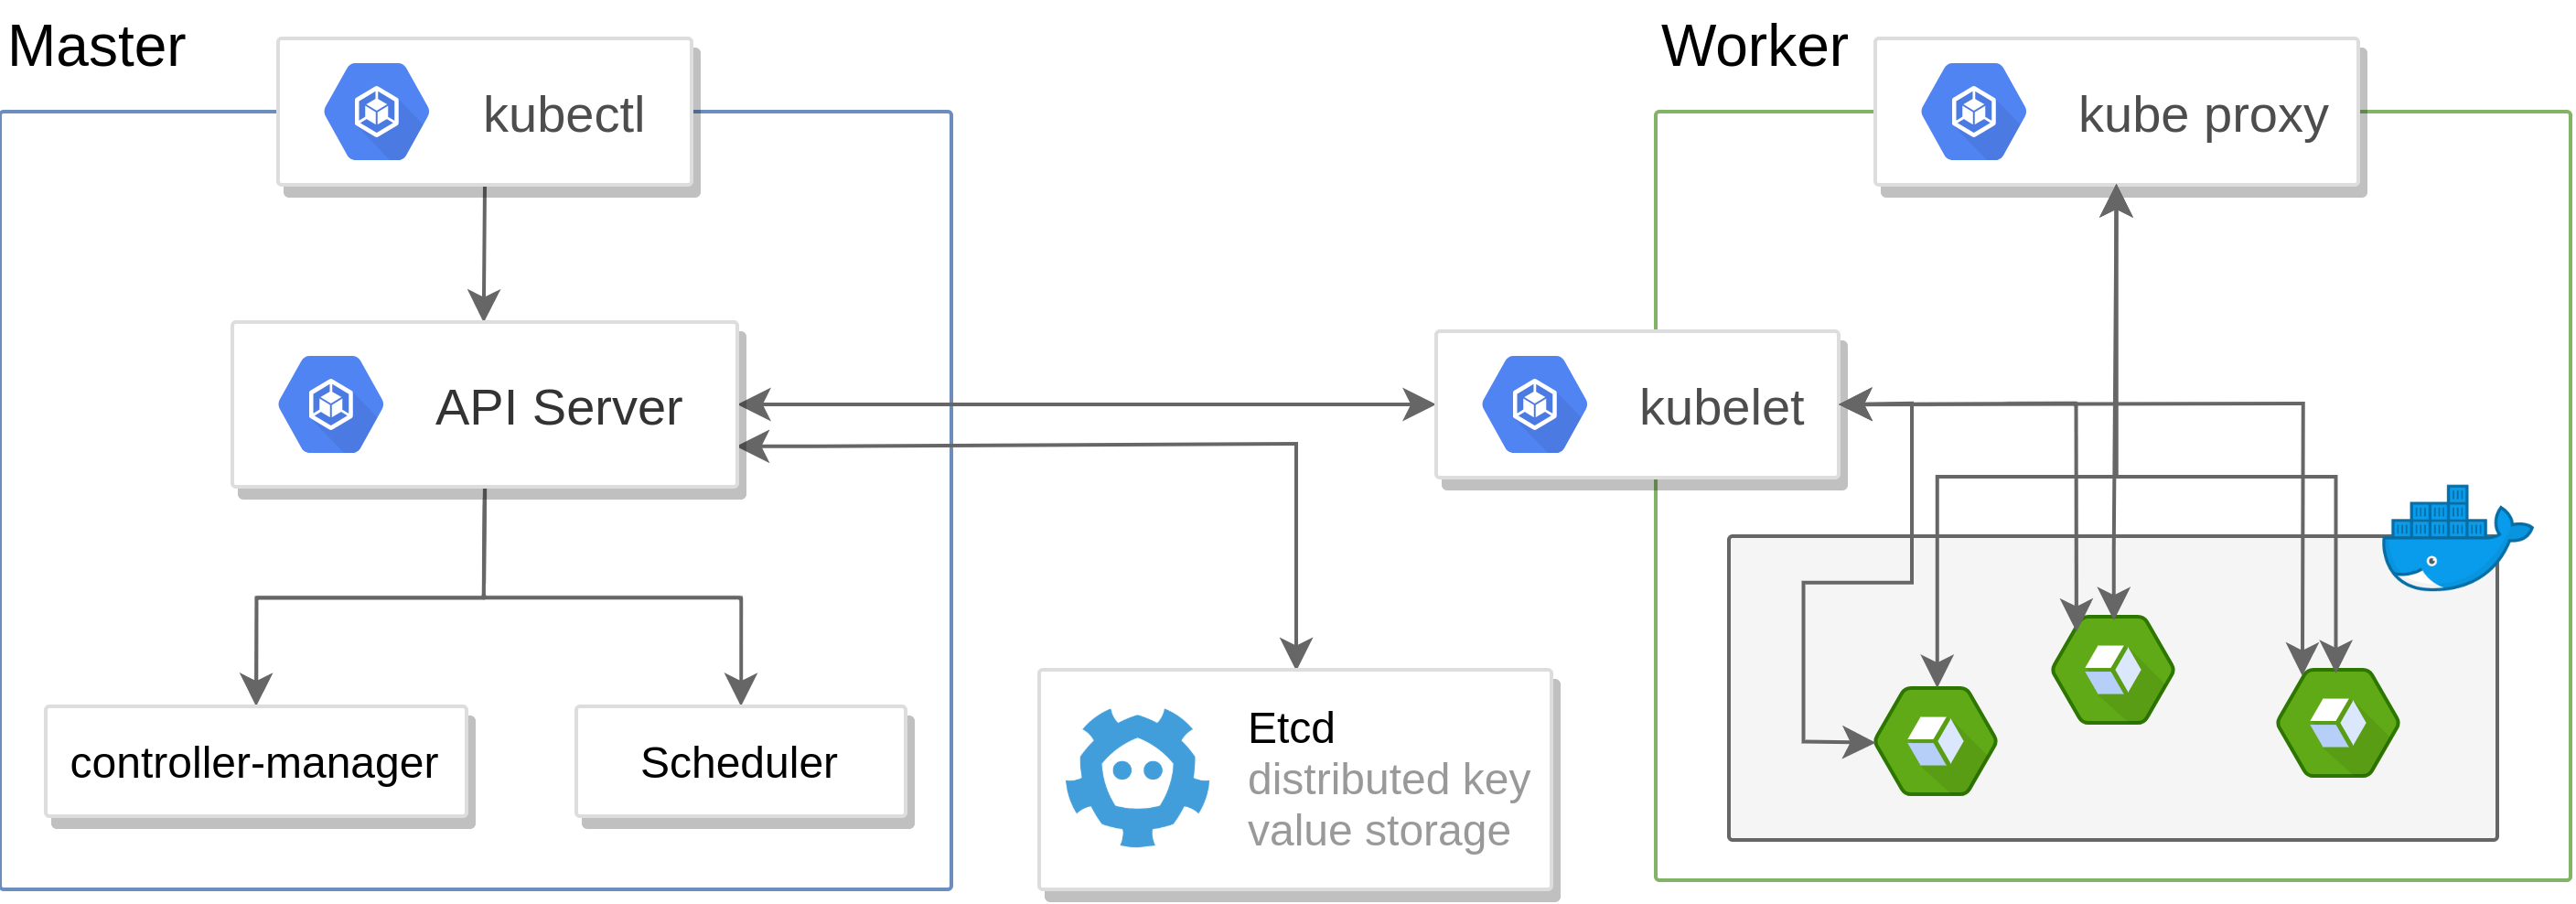
\includegraphics[width=\textwidth]{k8s_infrastructure.png}
    \caption{High-level diagram of K8s architecture}
    \label{fig:k8s_infrastructure}
\end{figure}

\subsubsubsection{Master Node Architecture}

\vspace{-5mm}\hspace{5mm} The sole entry point for the system in this setup is through an \textbf{API server} hosted by the master node. This server processes REST requests, validates them, and executes the bound business logic. For instance, a request to list all pods in the API whose name is v1 is 'GET /api/v1/pods'. 

This node also hosts some \textbf{etcd storage} which are distributed key-value stores storing shared configurations and service discovery which can be queried via REST. The previous example would in reality be routed to the etcd storage because it stores information regarding pods, jobs and their scheduling, etc...

As in any distributed system, resources in k8s clusters are scarce and require a \textbf{scheduler} which decides where to deploy a component thanks to information gathered regarding available resources on worker nodes. An extra level of control can also be achieved by the \textbf{controller-manager} which watches the shared state of the cluster and makes decisions and changes in order to reach the desired state. 

\subsubsubsection{Worker Node Architecture}

\vspace{-5mm}\hspace{5mm} Worker/Slave nodes are where pods are run, so \textbf{Docker} is used to provision and start containers here. Since these nodes depends on scheduling by the master node, this communication is guaranteed by \textbf{kubelet} which gets the configuration of a pod from the apiserver and ensures that the described containers are up and running and fetches information from the master etcd. Finally the \textbf{kube-proxy} service deals with individual host sub-netting and expose services to the external world. 

\subsubsection{Base security mechanisms}
\subsubsubsection{RBAC and the Kubernetes API}

\vspace{-5mm}\hspace{5mm}The Kubernetes API represents a fundamental fabric of Kubernetes through which all REST API calls, including object declarations are handled. As such, managing access to this component is primordial in order to maintain a secure Kubernetes cluster. Two categories of API users is distinguishable: human \textbf{users} and \textbf{service accounts} (used by pods within the cluster). Both of which has to go through three phases in order to gain access to the cluster (Authentication, Authorization, Admission Control).

\vspace{3mm}
In order to access the cluster (either through kubectl, client libraries or REST request), an user has to authenticate using at least one of the allowed methods. First of all, the k8s-api serves on port 443 with a TLS certificate which is required by the user in order to suceed the handshake. 

\begin{enumerate}
    \item \textbf{Authentication} - Contrary to other concepts in k8s, users are neither referenced nor stored by the API as an object. Thus, the authentication technically boils down to an HTTP request which is analysed by its auth modules (client certificates, token, etc.) in order to garantee that the requests comes from a specific user. For serviceaccounts, this is done through a \textbf{service account token} which can be mounted on the path `/var/run/secrets/kubernetes.io/serviceaccount` to allow automatic authentication.
    
    \item \textbf{Authorisation} - Once the first step is complete, the aforementioned request must be authorised by one of the following methods: \textbf{Node authorization} (internal authorization that allows for kubelet to query the API), \textbf{ABAC}  (authorization based on request attributes) and \textbf{RBAC} (authorization based on roles)
\end{enumerate}

\vspace{5mm}
The \textbf{role based access control} (RBAC) is one of the most granular method of authorization and can be leveraged to allow for pods within the cluster to communicate with the API. Defining this method of access regulation requires: 

\begin{enumerate}
    \item \textbf{Role}: \newline An assignment of a list of interactions (verbs) that can be applied to an array of resources in specific apiGroups. This can be restricted to a namespace or applied cluster wide (\textbf{Cluster Role}). For instance, the following yaml declares a role that allows for getting and listing deployments (that are in the apps/v1 API namespace): 
      \begin{minted}[gobble=4,frame=single,linenos ,fontsize=\footnotesize]{yaml}
      rules:
      - apiGroups: ["apps/v1"]
        resources: ["deployments"]
        verbs: ["get", "list"]
      \end{minted}
      
     \item \textbf{Service Account} and a \textbf{RoleBinding}: the separation of the role, the rolebinding and the service account allows for fine grained access control to the API and easy revocation. Using the RBAC properly therefore allows for programmatically managing the cluster within the cluster itself in a completely secure manner.
\end{enumerate}

\subsubsubsection{Pod Security Policy}

\hspace{5mm} Fine-grained access control is also implemented on the pod and container level through Pod security policies. This is done through defining a series of conditions which the affected pod must present in order to be accepted to the system. Policy enforcement is therefore done directly at the admission controller (before the creation of the resource) and independently of the container at hand. These policies can be summarized in the following overlying themes:

\begin{itemize}
\renewcommand\labelitemi{--}
    \item \textbf{Privilege} and \textbf{Escalation}: \newline policy inherited from the underlying docker component which would grant a container all capabilities that the host possesses and lifts all the limitations enforced by the device cgroup controller (see Appendix (\ref{appendix:libcontainer})). As a rule of thumb, no container that requires leverage over the host network stack should be privileged.
    
    Privilege escalation is by default banned through preventing the setuid binaries from changing the effective UID within the container. This feature is however prone to vulnerabilities as seen in the CVE-2019-5736 \autocite{CVE-2019-5736} through which exploits of the runC library could be used to obtain root execution from a docker container.
    
        \item \textbf{Volume} and \textbf{filesystem}: \newline allows managing access to certain kubernetes volume types, enforcement of file system group as well as restricting access permissions on different paths.
\end{itemize}

\subsection{Benchmark data}

\begin{listing}[H]
\begin{minted}[frame=single,fontsize=\footnotesize]{yaml}
temp_file_limit: 48593190
work_mem: 64
maintenance_work_mem: 1024
max_connections: 100
random_page_cost: 2
autovacuum_max_workers: 8
log_autovacuum_min_duration: 1
autovacuum_analyze_scale_factor: 0.15
\end{minted}
\caption{Production configuration used for postgres}
\label{list:prod}
\end{listing}


% \begin{figure}[!h]
%     \centering
%     \subfloat[native helm]{\includesvg[width=0.9\textwidth]{bench_vulas_latency_helm.svg}\label{fig:bench_vulas_latency_helm}}
    
%     \subfloat[hosted unoptimized]{\includesvg[width=0.9\textwidth]{bench_vulas_latency_unoptimized.svg}\label{fig:bench_vulas_unoptimized}}
    
%     \subfloat[hosted optimized]{\includesvg[width=0.9\textwidth]{bench_vulas_latency_optimized.svg}\label{fig:bench_vulas_optimized}}
%     \caption{Average latency (ms) grouped per deployment type}
%     \label{fig:bench_vulas_latency_grouped}
% \end{figure}

% \begin{figure}
%     \centering
%     \includegraphics[width=0.9\textwidth]{benchmark_vulas_latency_complexity.png}
%     \caption{Latency gain over reference deployment grouped by query complexity}
%     \label{fig:bench_vulas_latency_complexity}
% \end{figure}

\begin{table}[h]
\centering
\begin{tabular}{|c|c|c|c|c|}
\hline
\textbf{type}                   & \textbf{pattern}                                                                    & \textbf{provider} & \textbf{median} & \textbf{p95} \\ \hline
\multirow{9}{*}{\textbf{read}}  & \multirow{3}{*}{\textbf{random}}                                                    & aws               & 644             & 8256         \\ \cline{3-5} 
                                &                                                                                     & azure             & 3024            & 17792        \\ \cline{3-5} 
                                &                                                                                     & gcp               & 11328           & 30848        \\ \cline{2-5} 
                                & \multirow{3}{*}{\textbf{sequential}}                                                & aws               & 354304          & 2244608      \\ \cline{3-5} 
                                &                                                                                     & azure             & 72192           & 284672       \\ \cline{3-5} 
                                &                                                                                     & gcp               & 268288          & 378880       \\ \cline{2-5} 
                                & \multirow{3}{*}{\textbf{\begin{tabular}[c]{@{}c@{}}random\\ parallel\end{tabular}}} & aws               & 18560           & 31360        \\ \cline{3-5} 
                                &                                                                                     & azure             & 90624           & 199680       \\ \cline{3-5} 
                                &                                                                                     & gcp               & 76288           & 100864       \\ \hline
\multirow{6}{*}{\textbf{write}} & \multirow{3}{*}{\textbf{random}}                                                    & aws               & 724             & 972          \\ \cline{3-5} 
                                &                                                                                     & azure             & 2768            & 4128         \\ \cline{3-5} 
                                &                                                                                     & gcp               & 502             & 1608         \\ \cline{2-5} 
                                & \multirow{3}{*}{\textbf{sequential}}                                                & aws               & 382976          & 2736128      \\ \cline{3-5} 
                                &                                                                                     & azure             & 31104           & 1859584      \\ \cline{3-5} 
                                &                                                                                     & gcp               & 444416          & 634880       \\ \hline
\end{tabular}
\caption{Summary of latency distribution (ms) per access pattern per provider}
\label{tab:bench_fio}
\end{table}

\pagebreak
\printbibliography
\end{document}

